\documentclass[onecolumn,12pt]{article}
% \documentclass[twocolumn,10pt]{article}
\usepackage[utf8]{inputenc}  % Enable UTF-8 typing
\usepackage{emptypage}
\usepackage{graphicx}
% \usepackage[OT2,T1]{fontenc} 
\usepackage[hidelinks]{hyperref}        % Interactive PDF
% \usepackage[xetex]{hyperref}        % Interactive PDF
% \usepackage[dvipdfm]{hyperref}
% \usepackage[landscape,top=10.0mm, bottom=15.0mm, left=10.0mm, right=10.0mm]{geometry}
\usepackage[top=10.0mm, bottom=15.0mm, left=8.0mm, right=10.0mm]{geometry}
%\usepackage{savetrees}      % Enable to save paper!

%% Songbook packages
\usepackage[chorded]{songs}

\renewcommand{\familydefault}{\sfdefault}

% \usepackage{minted}
% \usepackage{musixtex}

% -- font nazvu obsahu
\renewcommand{\idxtitlefont}{\sffamily\large}

% -- font cisla pisnicky (vedle nazvu)
% \renewcommand{\thesongnum}{\hyperlink{page.2}}   % -- neco okolo
\renewcommand{\printsongnum}[1]{\sffamily\LARGE\hyperlink{page.2}#1}    % -- font
% \setlength{\songnumwidth}{0.5cm}                % -- sirka ohraniceni

% -- font autora 
\makeatletter\renewcommand\showauthors{\setbox\SB@box\hbox{\sfcode`.\@m\large\hyperlink{page.2}\songauthors}\ifdim\wd\SB@box>\z@\unhbox\SB@box\par\fi}\makeatother


% -- font nazev pisne
\renewcommand{\stitlefont}[1]{\bf\sffamily\Large\hyperlink{page.2}#1}

% -- font pisne sloky
\renewcommand{\lyricfont}{\sffamily\large}
\renewcommand{\everychorus}{\vspace{0.2cm}} % -- na zacatku refrenu
% \renewcommand{\everychorus}{{\textnote{\textbf{R:}}}} % -- na zacatku refrenu
% \renewcommand{\printversenum}[1]{\textbf{}}     % -- na zacatku sloky
\renewcommand{\printversenum}[1]{\textbf{\hspace{-0.0cm}#1:\,}}     % -- na zacatku sloky
% \renewcommand{\chorusfont}{\it}               % -- font refrenu, podobne sloka atd

% -- font akordu 
\renewcommand{\printchord}[1]{\sffamily\small\bf#1}

% -- mezery
% -- posunuti sloky doprava
\setlength{\versenumwidth}{0.5cm}

% -- mezera mezi refrenem a slokou
\versesep=17pt plus 14pt minus -14pt

% -- zacatek pisne 
% \beforepostludeskip=-15pt plus 15pt minus 0pt

% -- odskok akord 
\baselineadj=-20pt plus 12pt minus 0pt

% -- cary
\setlength{\cbarwidth}{2pt}
\setlength{\sbarheight}{0pt}



% -- penalties
% \interlinepenalty=-1000
% \brkpenalty=100000

% \renewcommand{\clineparams}{
%   \baselineskip=0pt
%   \lineskiplimit=0pt
%   \lineskip=0pt
% }

%% Song aesthetics
% \noversenumbers
% \setlength\baselineadj{0.0em}
% \renewcommand{\colbotglue}{2pt plus .5\textheight minus 2pt}


%% Song index settings
\newindex{titleidx}{titleidx} % Index name
\indexsongsas{titleidx}{\thepage}

% \renewcommand{\chorusjustify}{\justifycenter}

% \renewcommand{\clineparams}{
  % \baselineskip=1pt
%   \lineskiplimit=1pt
%   \lineskip=1pt
% }


% \renewcommand\makeprelude{%
%   \resettitles
%   \centering
%   {\Large\bfseries\thesongnum. \songtitle\par
%    \nexttitle\foreachtitle{(\songtitle)\par}}%
%   \extendprelude
% }
% \sepindexesfalse

%% Author, songbook title, year, etc.
% \title{\textbf{\Huge All you need is guitar \dots \quad\quad\quad\quad \\[1cm] \quad\quad\quad \dots and few chords}\\[1.5cm]\Large{Tomíkův zpěvník}\\\the\year\\[1cm]\includegraphics[width=0.8\textwidth]{imgs/logo.png}\thispagestyle{empty}}
% \title{\textbf{\Huge All you need is guitar \dots \quad\quad\quad\quad \\[1cm] \quad\quad\quad \dots and few chords}\\[1.5cm]\Large{Zpěvník Hrůzy}\\\the\year\\[1cm]\includegraphics[width=0.8\textwidth]{imgs/logo.png}}
\title{\textbf{\Huge All you need is guitar \dots \quad\quad\quad\quad \\[1cm] \quad\quad\quad \dots and few chords}\\[1.5cm]\Large{Tomíkův zpěvník}\\\the\year\\[1cm]\includegraphics[width=0.8\textwidth]{imgs/logo.png}}
\author{\thispagestyle{empty}}
\date{}

\begin{document}
\songcolumns{2}
% % \onecolumn
% \songcolumns{1}
% \flushbottom
% \twocolumn[\LARGE\centering My Songs]
%% Front page: title, etc.
\pagenumbering{gobble}
  \maketitle
  

  % \vspace{4cm}

%% Songbook owner's signature
%   \begin{center}
%     {\huge{This songbook belongs to}}\\
%     \vspace{1cm}
% {\begin{music}\trebleclef\end{music}\huge{\dots\dots\dots\dots\dots\dots\dots\dots\dots\dots}\begin{music}\trebleclef\end{music}}
%    \end{center}
\clearpage
\pagenumbering{arabic}
%% Include rules section
% \include{rules}

%% Display table of content + song index
% \setcounter{tocdepth}{1}
% \tableofcontents
\showindex[2]{Songs}{titleidx}

% \showindex{Songs}{titlfile}
% \showindex{Lactani}{titleidx}

% Index file for Songbook.pdf
% Automatically generated at Sun Jan 15 23:41:09 CST 2023 by link-doc
% Do not attempt to alter this file as it will be regenerated upon next compilation by link-doc
\input{songs/00-title}
\sclearpage\beginsong{1 Signální}[by={Chinaski}]\capo{1}
\beginverse
Až si \[G]zejtra ráno \[C]řeknu zase \[Em]jednou provždy dost\brk
\[G]právem se mi \[C]budeš tiše \[Em]smát\brk
jak \[G]omluvit si \[C]svoji slabost, \[Em]nenávist a zlost\brk
když \[G]za všechno si \[C]můzu vlastně \[Em]sám.\brk
\endverse
\beginchorus
Za \[Am]spoustu dní možná za \[C]spoustu let\brk
až se mi \[G]rozední budu ti \[D]vyprávět\brk
na 1. \[Am]signalní jak jsem \[C]vobletěl svět\brk
jak tě to \[G]vomámí a \[D]nepustí zpět.\brk
Jaký si to \[F]udeláš \[Bb]takový to \[Dm]máš.\brk
Jaký si to \[F]udeláš \[Bb]takový to \[Dm]máš.\brk
\endchorus
\beginverse
Až se \[G]dneska večer \[C]budu tvářit \[Em]zas jak Karel Gott,\brk
\[G]budu zpívat \[C]vampampyda\[Em]pam\brk
všechna \[G]sláva polní \[C]tráva ale \[Em]peníz přijde vhod\brk
\[G]jak jsem si to \[C]udělal tak to \[Em]mám.\brk
\endverse
\beginchorus
Za \[Am]spoustu dní možná za \[C]spoustu let\brk
až se mi \[G]rozední budu ti \[D]vyprávět\brk
na 1. \[Am]signalní jak jsem \[C]vobletěl svět\brk
jak tě to \[G]vomámí a \[D]nepustí zpět.\brk
Jaký si to \[F]udeláš \[Bb]takový to \[Dm]máš.\brk
Jaký si to \[F]udeláš \[Bb]takový to \[Dm]máš.\brk
\[F] \[Dmi]   \[F] \[Dmi]         \brk
\endchorus
\beginchorus
Za \[Am]spoustu dní možná za \[C]spoustu let\brk
až se mi \[G]rozední budu ti \[D]vyprávět\brk
na 1. \[Am]signalní jak jsem \[C]vobletěl svět\brk
jak tě to \[G]vomámí a \[D]nepustí zpět.\brk
nán\[Am]ana\[C]..\[G]. \[D] \[Am]  \[C] \[G] \[D]         \brk
Jaký si to \[F]udeláš \[Bb]takový to \[Dm]máš.\brk
Jaký si to \[F]udeláš \[Bb]takový to \[Dm]         \brk
\endchorus\endsong
\sclearpage\beginsong{Accidentally In Love}[by={Counting Crows}]
\beginverse*{\nolyrics Intro: \[G]\[C]\[Em]\[A]\[C]      
}\endverse
\beginverse
\[G]So she said what's the pr\[C]oblem baby\brk
\[G]What's the problem I don't kno\[C]w\brk
Well maybe I'm in\[Em] love (love)\brk
Think about it \[A]everytime I think about it\brk
\[C]Can't stop thinking 'bout it\brk
\endverse
\beginverse
\[G]How much longer will it ta\[C]ke to cure this?\brk
\[G]Just to cure it 'cause I ca\[C]n't ignore it if it's lo\[Em]ve (love)\brk
Makes me wanna \[A]turn around and face me but I \[D]don't know\brk
Nothing 'bout \[C]love            Ahhhh\brk
\endverse
\beginchorus
\[G]Come on,\[Am] come on\brk
\[C]Turn a little \[D]faster\brk
\[G]Come on, \[Am]come on\brk
The \[C]world will follow \[D]after\brk
\[G]Come on, \[Am]come on\brk
\[C]'Cause everybody's\[D] after\[Em] lov\[A]e  \[C]         \brk
\endchorus
\beginverse
\[G]So I said I'm a sn\[C]owball running\brk
\[G]Running down into the spr\[C]ing that's coming all this lo\[Em]ve\brk
Melting under \[A]blue skies belting out \[C]sunlight\brk
shimmering \[G]love\brk
\endverse
\beginverse
Well baby \[C]I surrender to the \[G]strawberry ice cream\brk
\[C]never ever end of all this\[Em] love\brk
Well I \[A]didn't mean to do it\brk
But there's\[D] no escaping your\[C] love   ahhhhh\brk
\endverse
\beginverse*{\nolyrics [Bridge]: 
\[Em]These line of li\[C]ghtning mean we're\brk
\[G]never alone, \[Am]never alone\brk
}\endverse
\beginchorus
\[G]Come on, \[Am]come on\brk
\[C]Move a little \[D]closer\brk
\[G]Come on, \[Am]come on\brk
I wa\[C]nt to hear you \[D]whisper\brk
\[G]Come on, \[Am]come on\brk
\[C]Settle down ins\[D]ide my \[Em]love\[D]            Ahhhh\brk
\[G]Come on, \[Am]come on\brk
\[C]Jump a little \[D]higher\brk
\[G]Come on, \[Am]come on\brk
If you \[C]feel a little \[D]lighter\brk
\[G]Come on, \[Am]come on\brk
We \[C]were once upon a \[D]time in \[Em]love\[A]   \[C]         \brk
\endchorus
\beginverse*{\nolyrics [Bridge]: 
We're accidentally i\[G]n love  \[C]         \brk
Accidentally i\[Em]n love  \[D]         \brk
Accidentally i\[G]n love  \[C]         \brk
Accidentally i\[Em]n love  \[D]         \brk
Accidentally i\[G]n love  \[C]         \brk
Accidentally i\[Em]n love  \[D]         \brk
Accidentally i\[G]n love  \[C]         \brk
Accidentally i\[Em]n love  \[D]         \brk
Accidentally,\[G] I'm in love, I'm in l\[C]ove\brk
I'm in love, I'm in l\[Em]ove\brk
I'm in love, I'm in l\[D]ove\brk
Accidentally,\[G] I'm in love, I'm in l\[C]ove\brk
I'm in love, I'm in l\[Em]ove\brk
I'm in love, I'm in l\[D]ove, accidentally\brk
}\endverse
\beginchorus
\[G]Come on, \[Am]come on\brk
\[C]Spin a little \[D]tighter\brk
\[G]Come on, \[Am]come on\brk
And the \[C]world's a little \[D]brighter\brk
\[G]Come on, \[Am]come on\brk
Just \[C]get yourself in\[D]side her \[Em]love..\[D]...I'm in love\[G][/ta\brk
\endchorus\endsong
\sclearpage\beginsong{Africa}[by={Toto}]
\capo{2}
\beginverse*{\nolyrics Intro: \[G] \[F#m]\[Hm] 
}\endverse
\beginverse
\[A]I hear the drums ech\[C#m]oing ton\[F#m]ight
\[A/E]She hears only whi\[G]spers of some \[D]quiet conver\[Dmaj]satio\[G] \[F#m]n\[Hm]         
\[A]She's coming in, \[C#m]twelve thirty \[F#m]flight
The moon\[A/E]lit wings re\[G]flect the stars that \[D]guide me toward sal\[Dmaj]vation\[G]\[F#m]\[Hm]         
\[A]I stopped an \[C#m]old man along the \[F#m]way
Hoping \[A/E]to find some \[G]old forgotten \[D]words or ancient \[Dmaj]melo - \[G]die\[F#m]s\[Hm]         
\[A]He turned to \[C#m]me as if to \[F#m]say, hurry boy, \[G]it's waiting there for you \[F#m]\[Hm]
\endverse
\beginchorus
\[Emi]Gonna take a l\[C]ot to drag me a\[G]way from \[D]you
\[Emi]There's nothing that a \[C]hundred men or \[G]more could ever \[D]do
\[Emi]I bless the r\[C]ains down i\[G]n  Afri\[D]ca
\[Emi]Gonna take some \[C]time to do the t\[G]hings we never \[Hm]had..\[D].\[Emi]\[D]\[G]         
Ooo \[G]Oo\[F#m]o\[Hm]         
\[G] \[F#m]   \[Hm]         
\endchorus
\beginverse
\[A]The wild dogs \[C#m]cry out in the \[F#m]night
As \[A/E]they grow restless \[G]longing for some \[D]solitary \[Dmaj]compa-\[G]ny\[F#m]\[Hm]         
\[A]I know that \[C#m]I must do what's \[F#m]right
As sure as \[A/E]Kilimanjaro \[G]rises like O\[D]lympus above the Se\[Dmaj]r - enge\[G]ti\[F#m]\[Hm]         
\[A]I seek to \[C#m]cure what's deep in\[F#m]side
\[F#m]Frightened of this \[G]thing that I've be\[F#m]\[Hm]come
\endverse
\beginchorus
\[Emi]Gonna take a l\[C]ot to drag me a\[G]way from \[D]you
\[Emi]There's nothing that a \[C]hundred men or \[G]more could ever \[D]do
\[Emi]I bless the r\[C]ains down i\[G]n  Afri\[D]ca
\[Emi]Gonna take some \[C]time to do the t\[G]hings we never \[Hm]had..\[D].\[Em]\[D]\[G]  \[F#m]   \[Hm]   
\endchorus
\beginchorus
\[Emi]Gonna take a l\[C]ot to drag me a\[G]way from \[D]you
\[Emi]There's nothing that a \[C]hundred men or \[G]more could ever \[D]do
\[Emi]I bless the r\[C]ains down i\[G]n  Afri\[D]ca
\[Emi]Gonna take some \[C]time to do the t\[G]hings we never \[Hm]had..\[D].\[Em]\[D]\[G]  
\endchorus
\endsong
\sclearpage\beginsong{Až Mi Bude Pětašedesát}[by={Michal Horák}]
\beginverse
\[C]Budu pořád \[Caug]štramák jako d\[F]nes,\[Fm]\brk
\[C]Co se v klidu \[Caug]do ix-eska \[F]vlez\[Fm],\brk
A \[C]budu efko \[E/B]na kytaře \[F]pořád blbě \[D]hrát,\brk
No a \[C/G]budu \[E/G#]pořád \[Am]nad vě\[C7/G]cí,\brk
Až mi \[F]bude pěta\[F/G]šede\[C]sát?\brk
\endverse
\beginverse
\[C]Budu trapný \[Caug]vtipy říkat \[F]dál,\[Fm]\brk
\[C]Aniž by se \[Caug]jim kdokoliv \[F]smál\[Fm],\brk
A \[C]budu se jim \[E/B]dál jenom já \[F]smát, a jak \[D]rád,\brk
No a \[C/G]budu \[E/G#]pořád \[Am]nad vě\[C7/G]cí,\brk
Až mi \[F]bude pěta\[F/G]šede\[C]sát?\brk
\endverse
\beginchorus
No a \[E7]pokud není \[Am]jasný\brk
Zda to \[E7]oznamuju, či se \[Am]ptám,\brk
Přišel jsem \[C/G]na ře\[E/G#]šení \[Am]spás\[C7/G]ný,\brk
Bude to \[F]tak, jak si to \[F/G]udě \[C]lám.\brk
\endchorus
\beginverse
\[C]Budu pořád \[Caug]baštit špage\[F]ty  \[Fm]         \brk
\[C]A benzínk\[Caug]ový baget\[F]y? (Hmm golfik, j\[Fm]oohellip;)\brk
\[C]A budu za to \[E/B]všem stravenky \[F]cpát, i když \[D]nechtěj,\brk
No a \[C/G]budu \[E/G#]pořád \[Am]nad vě\[C7/G]cí,\brk
Až mi \[F]bude pěta\[F/G]šede\[C]sát?\brk
\[C/G]   \[E/G#]    \[Am]    \[C7/G]     \[F]   \[F/G]    \[C]         \brk
\endverse
\beginchorus
No a \[E7]pokud není \[Am]jasný\brk
Zda to \[E7]oznamuju, či se \[Am]ptám,\brk
Přišel jsem \[C/G]na ře\[E/G#]šení \[Am]spás\[C7/G]ný,\brk
Bude to \[F]tak, jak si to \[F/G]udě \[C]lám.\brk
\endchorus
\beginverse
\[C]Budu pořád \[Caug]fichtly stavět \[F]si  \[Fm]         \brk
\[C]A neřešit \[Caug]zbytečný vě\[F]ci (jako motor)\[Fm],\brk
A \[C]budu chtít pak \[E/B]u piva, ať se \[F]na to někdo \[D]podivá,\brk
No a \[C/G]budu \[E/G#]pořád \[Am]nad vě\[C7/G]cí,\brk
Až mi \[F]bude pěta\[F/G]šede\[C]sát?\brk
Až mi \[Dm7]bude pěta\[G4]šede\[C]sát?\brk
Až mi \[Dm7]bude pěta\[G4]šede, \[Dm7]snad se to po\[G4]vede,\brk
\endverse\endsong
\sclearpage\beginsong{Bad Bad Leroy Brown}[by={Jim Croce}]
\beginverse*{\nolyrics Intro: \[G] \[D7]         \brk
}\endverse
\beginverse
Well, the \[G]south side of Chicago\brk
Is the \[A7]baddest part of town.\brk
And if you \[B7]go down there\brk
You better \[C]just beware of a \[D7]man name of \[C]Leroy Bro\[G]wn.\[D7]\brk
Now, \[G]Leroy more than trouble,\brk
You see he \[A7]stand about 'bout six foot four.\brk
All the \[B7]downtown ladies cal\[C]l him "treetop lover."
All the \[D7]men just \[C]call him sir.\[G]  \[D7]         \brk
\endverse
\beginchorus
And he's \[G]bad, bad, Leroy Brown,\brk
The \[A7]baddest man in the whole damn town.\brk
\[B7]Badder than old King \[C]Kong\brk
And \[D7]meaner than a \[C]junkyard do\[G]g. \[D7]         \brk
\endchorus
\beginverse
Now, \[G]Leroy, he a gambler,\brk
and he \[A7]like his fancy clothes.\brk
And he \[B7]like to wave \[C]diamond rings\brk
in front of \[D7]every\[C]body's \[G]nos\[D7]e\brk
He got a \[G]custom Continental.\brk
He got an \[A7]Eldorado too.\brk
He got a \[B7]thirty-two gun in his \[C]pocket for fun.\brk
He got a \[D7]razor \[C]in his \[G]shoe.\[D7]\brk
\endverse
\beginchorus
And he's \[G]bad, bad, Leroy Brown,\brk
The \[A7]baddest man in the whole damn town.\brk
\[B7]Badder than old King \[C]Kong\brk
And \[D7]meaner than a \[C]junkyard do\[G]g. \[D7]         \brk
\endchorus
\beginverse
Well, \[G]Friday 'bout a week ago,\brk
\[A7]Leroy's shootin' dice.\brk
And at the \[B7]edge of the bar sat a \[C]girl name of Doris\brk
and \[D7]oh, that \[C]girl look \[G]nice\[D7]\brk
Well, he \[G]cast his eyes upon her\brk
and the \[A7]trouble soon began.\brk
And \[B7]Leroy Brown, he learned a \[C]lesson 'bout messin'\brk
with the \[D7]wife of a \[C]jealous \[G]man \[D7]         \brk
\endverse
\beginchorus
And he's \[G]bad, bad, Leroy Brown,\brk
The \[A7]baddest man in the whole damn town.\brk
\[B7]Badder than old King \[C]Kong\brk
And \[D7]meaner than a \[C]junkyard do\[G]g. \[D7]         \brk
\endchorus
\beginverse
Well, the \[G]two men took to fightin'\brk
And when they \[A7]pulled them from the floor,\brk
\[B7]Leroy looked like a \[C]jigsaw puzzle with a \[D7]couple of \[C]pieces \[G]gone\[D7].\brk
\endverse
\beginchorus
And he's \[G]bad, bad, Leroy Brown,\brk
The \[A7]baddest man in the whole damn town.\brk
\[B7]Badder than old King Kon\[C]g\brk
And \[D7]meaner than a \[C]junkyard do\[G]g. \[D7]         \brk
And he's \[G]bad, bad, Leroy Brown,\brk
The \[A7]baddest man in the whole damn town.\brk
\[B7]Badder than old King Kon\[C]g\brk
And \[D7]meaner than a \[C]junkyard do\[G]g.\brk
\endchorus
\endsong
\sclearpage\beginsong{Baroko}[by={Richard Muller}]
\beginverse*{\nolyrics Intro: \[Dmi]    \[C]  \[Dmi]    \[C]         \brk
}\endverse
\beginverse
\[Dmi]Schoulené holky spí \[C]nahé \brk
u h\[Dmi]robu Tycha de Bra\[C]he \brk
z k\[Bb]amene oživlá světi\[C]ce \brk
poz\[Dmi]vedá monstranci měsí\[C]ce \brk
\endverse
\beginchorus
T\[F]aková z\[C]ář je jen \[Dmi]jedna \[Bb]\brk
odtu\[F]d až do \[C]nedohled\[Dmi]na    \[Bb]         \brk
no a\[F] z něj dale\[C]ko šir\[Dmi]oko     \[Bb]         \brk
prou\[F]dem se rozl\[C]évá baro\[Dmi]ko     \[Bb]         \brk
\endchorus
\beginverse
\[Dmi]Andělé odhalte tv\[C]áře \brk
pro\[Dmi] slepé harmonikář\[C]e \brk
Kte\[Bb]ré jsem čekal a ne\[C]propás \brk
Dův\[Dmi]erně známý je kaž\[C]dý z vás \brk
\endverse
\beginchorus
J\[F]ste-li \[C]tak důvěrný \[Dmi]známý \[Bb]\brk
Pojď\[F]te a zp\[C]ívejte s nám\[Dmi]i     \[Bb]         \brk
My d\[F]ole vy \[C]zase vysoko\[Dmi]      \[Bb]         \brk
O to\[F]m jak m\[C]ocné je baro\[Dmi]ko     \[Bb]         \brk
\endchorus
\beginverse
\[Dmi]Sedlejme koně a v\[C]zhůru \brk
Zap\[Dmi]lašme zlou denní můr\[C]u \brk
Kte\[Bb]rá nám sežrala sto\[C]letí \brk
Zpě\[Dmi]nění hřebci se roz\[C]letí \brk
\endverse
\beginchorus
V\[F] tuto n\[C]oc lámání \[Dmi]kostí \[Bb]\brk
Chyt\[F]rácké m\[C]alověrnost\[Dmi]i     \[Bb]         \brk
Sraž\[F]me tu b\[C]estii hlubo\[Dmi]ko    \[Bb]         \brk
Tak \[F]jak to \[C]umí jen bar\[Dmi]oko   \[Bb]         \brk
Dne\[Bb]s je dnes, ale co\[C] zítra \brk
Zby\[Bb]de tu zázračná mitr\[C]a? \brk
Kom\[Bb]u dá svou hlavu do \[C]klína \brk
ryz\[Bb]áček svatého Mart\[C]ina \brk
\endchorus
\beginchorus
Z\[F]em kter\[C]á nemá své \[Dmi]nebe   \[Bb]         \brk
Ztra\[F]tila vš\[C]echno i seb\[Dmi]e      \[Bb]         \brk
Zaro\[F]stla pa\[C]stvou jen pr\[Dmi]o oko   \[Bb]         \brk
Proč\[F] si tak vzdá\[C]lené - v perutí\[Dmi]ch oděné \[Bb] baroko ? \brk
\endchorus
\beginchorus
Z\[F]em kter\[C]á nemá své \[Dmi]nebe  \[Bb]         \brk
Ztra\[F]tila vš\[C]echno i seb\[Dmi]e     \[Bb]         \brk
Zarů\[F]stá pas\[C]tvou jen pro ok\[Dmi]o     \[Bb]         \brk
   P\[F]roč si \[C]tak vzdálené ba\[Dmi]roko  \[Bb] \brk
\endchorus\endsong
\sclearpage\beginsong{Blíženci}[by={Olympic}]
\beginverse
\[C]Tys byla \[G]víc než krásně \[Am]bláznivá  \[Am/G]         \brk
\[F]i hloupá \[G]s žádnou pamě\[C]tí.\brk
\[C]Mít sílu, \[G]tak se zpátky \[Am]nedívám,  \[Am/G]         \brk
\[F]už chápu, \[G]co je prokle\[E]tí.\brk
\endverse
\beginchorus
\[Bb]Já \[F]zbouranej jsem tu \[C]dál.\brk
\[Bb]Já \[F]zbouranej jsem tu \[C]dál.\brk
\endchorus
\beginverse
\[C]Říkal jsem \[G]všem tvým plánům \[Am]tlachání  \[Am/G]         \brk
\[F]a bral tě \[G]vůbec s převa\[C]hou.\brk
\[C]Prohlížím \[G]loňskou fotku \[Am]z koupání \[Am/G]         \brk
\[F]a piju \[G]víno nad Pra\[E]hou.\brk
\endverse
\beginchorus
\[Bb]Já \[F]zbouranej jsem tu \[C]dál.\brk
\endchorus
\beginverse*{\nolyrics [Bridge]: 
\[Am]Víš, holka, \[F]vzal síly \[Am]ten pocit, \[F]že se mýlím,\brk
\[Am]jak já moh \[G]myslet, že tě \[C]znám.  \[E7]         \brk
\[Am]Ty tam a \[F]já tady, \[Am]spíš věřím \[F]na záhady,\brk
\[Am]a proto \[G]stejně sedím \[C]sám.  \[E7]         \brk
}\endverse
\beginverse
\[C]Nech příští \[G]záplavy svých \[Am]dopisů,   \[Am/G]         \brk
\[F]blížence \[G]dálka rozdvo\[C]jí.\brk
\[C]Léty se \[G]měníš v jeden \[Am]z obrysů, \[Am/G]         \brk
\[F]zatím si \[G]dobře nesto\[E]jím.\brk
\endverse
\beginchorus
\[Bb]Já \[F]zbouranej jsem tu \[C]dál.\brk
\[Bb]Já \[F]zbouranej jsem tu \[C]dál.\brk
\[Bb]Já \[F]zbouranej jsem tu \[C]dál.\brk
\endchorus
\beginverse*{\nolyrics [Outro]: 
Tak \[C]sám.
}\endverse\endsong
\sclearpage\beginsong{Boulevard Of Broken Dreams}[by={Green Day}]
\capo{3}
\transpose{5}
\beginverse*{\nolyrics Intro: \[Em]   \[G]  \[D]  \[A]\brk
}\endverse
\beginverse
\[Em]I walk a l\[G]onely road, the o\[D]nly one that I\[A] have ever know\[Em]n\brk
Don't know \[G]where it goes, \[D]but it's home to \[A]me and I walk al\[Em]one\brk
 \[Em]   \[G]  \[D]  \[A]\brk
\endverse
\beginverse
\[Em]I walk this e\[G]mpty street, o\[D]n the bouleva\[A]rd of broken dr\[Em]eams\brk
Where the \[G]city sleeps, and \[D]I'm the only o\[A]ne and I walk al\[Em]one\brk
I\[Em] wal\[G]k a\[D]lone, I walk\[A] alone        \[Em]\brk
I\[Em] wal\[G]k a\[D]lone, I walk\[A] a....\brk
\endverse
\beginchorus
\[C]My shado\[G]w's the only \[D]one that walks \[Em]beside me\brk
\[C]My shallo\[G]w heart'\[D]s the only thing\[Em] that's beating\brk
\[C]Sometimes\[G] I wish \[D]someone out there \[Em]will find me\brk
\[C]Till then \[G]I walk \[B7]alone\brk
A\[Em]h-Ah A\[G]h-Ah A\[D]h-Ah   A\[A]hhh-Ah\brk
haaa-\[Em]ah  A\[G]h-Ah A\[D]h-Ah   A\[A]h-Ah\brk
\endchorus
\beginverse
\[Em]I'm walking d\[G]own the line\brk
\[D]That divides me \[A]somewhere in my \[Em]mind\brk
On the \[G]border line \[D]of the edge\brk
And \[A]where I walk al\[Em]one\brk
 \[Em]   \[G]  \[D]  \[A]\brk
\endverse
\beginverse
\[Em]Read bet\[G]ween the lines\brk
\[D]What's fucked up and \[A]everything's al\[Em]right\brk
Check my \[G]vital signs, to \[D]know I'm still a\[A]live\brk
And I walk al\[Em]one\brk
I\[Em] wal\[G]k a\[D]lone, I walk\[A] alone        \[Em]\brk
I\[Em] wal\[G]k a\[D]lone, I walk\[A] a....\brk
\endverse
\beginchorus
\[C]My shado\[G]w's the only \[D]one that walks \[Em]beside me\brk
\[C]My shallo\[G]w heart'\[D]s the only thing\[Em] that's beating\brk
\[C]Sometimes\[G] I wish \[D]someone out there \[Em]will find me\brk
\[C]Till then \[G]I walk \[B7]alone\brk
A\[Em]h-Ah A\[G]h-Ah A\[D]h-Ah \[A]  Ahhh-Ah\brk
haaa-\[Em]ah  A\[G]h-Ah A\[D]h-Ah  I \[A]walk alone, I walk a...\brk
\[C]  \[G]  \[B]  \[B7]\brk
\endchorus
\beginverse
\[Em]I walk this \[G]empty street, \[D]on the boule\[A]vard of broken d\[Em]reams\brk
Where the c\[G]ity sleeps, and \[D]I'm the only on\[A]e and I walk a...\brk
\endverse
\beginchorus
\[C]My shado\[G]w's the only \[D]one that walks \[Em]beside me\brk
\[C]My shallo\[G]w heart'\[D]s the only thing\[Em] that's beating\brk
\[C]Sometimes\[G] I wish \[D]someone out there \[Em]will find me\brk
\[C]Till then \[G]I walk \[B7]alone\brk
\endchorus
\endsong
\sclearpage\beginsong{Brandy Youre A Fine Girl}[by={Looking Glass}]
\beginverse
There's a \[E]Port   on a \[G#m]Western\[C#m] bay  \brk
And it \[F#m]serves   a hundred \[D]ships a \[A]day\brk
Lonely s\[E]ailors   pass the \[G#m]time aw\[C#m]ay\brk
And \[F#m]talk a\[A]bout their \[E]homes\brk
And there's a g\[E]irl  in this \[G#m]harbor to\[C#m]wn\brk
And she w\[F#m]orks   layin' w\[D]hiskey do\[A]wn\brk
They say Br\[E]andy   fetch ano\[G#m]ther roun\[C#m]d\brk
She \[F#m]serves them whis\[A]key and wine\brk
\endverse
\beginchorus
The sailors say B\[C#m]randy you're a f\[A]ine girl (your're a fine girl)\brk
What a \[C#m]good wife you would \[A]be (such a fine girl)\brk
Your \[E]eyes could steal a \[B/E]sailor from the \[A]se\[E]a \[A](do,do...)\brk
\endchorus
\beginverse
\[E]Brandy wears a \[G#m]braided ch\[C#m]ain\brk
Made of \[F#m]finest \[A]silver from the \[D]north of \[A]Spain\brk
A \[E]locket that \[G#m]bears the na\[C#m]me\brk
Of the \[F#m]man that \[A]Brandy \[E]loves\brk
He \[E]came on a \[G#m]summer's d\[C#m]ay\brk
Bringing \[F#m]gifts from \[D]far a\[A]way\brk
But he \[E]made it clear he\[G#m] couldn't \[C#m]stay\brk
No \[F#m]harbor \[A]was his \[E]home\brk
\endverse
\,\\[0.7cm]
\textbf{R:} The sailors say ...
\beginverse*{\nolyrics [Bridge]: 
Yeah \[C#m]Brandy used to \[E/B]watch his eyes\brk
When he \[A]told his sailor's \[B]stories\brk
She could \[C#m]feel the ocean \[E/B]fall and rise\brk
She s\[A]aw it's raging \[B]glory\brk
But \[C#m]he had always \[D]told the truth\brk
Lord he \[C#m]was an honest \[A]man\brk
And \[E]Brandy does her \[B/E]best to under\[A]sta\[E]nd \[A](do,do...)\brk
}\endverse
\beginverse
At \[E]night when the\[G#m] bars close \[C#m]down\brk
\[F#m]Brandy \[A]walks through a \[D]silent \[A]town\brk
And \[E]loves a man who's\[G#m] not \[C#m]around\brk
She \[F#m]still can \[A]hear him \[E]say she hears him say\brk
\endverse
\beginchorus
She hears him say \[C#m]Brandy you're a \[A]fine girl (your're a fine girl)\brk
What a \[C#m]good wife you would \[A]be (such a fine girl)\brk
But my \[E]life my lover my \[B/E]lady is the \[A]sea\[E] (d\[A]o,do...)\brk
Say \[C#m]Brandy you're a \[A]fine girl (your're a fine girl)\brk
What a \[C#m]good wife you would \[A]be (such a fine girl)\brk
But my \[E]life my lover my \[B/E]lady is the \[A]sea\[E]  A\[A] D\[A] G \[E]B  Youre A Fine   Youre A Fine   Youre A Fine   Youre A Fine   Youre A Fine   chords follow\brk
\endchorus\endsong
\input{songs/Budu_Všechno_Co_Si_Budeš_Přát}
\input{songs/Bára}
\sclearpage\beginsong{Co Z Tebe Bude}[by={Pokáč}]
\capo{3}
\beginverse
\[C]Když jsem byl prcek,\[Dm] tak se mě všude\brk
\[G]Dospěláci ptali chlapče,\[C] co z tebe bude\brk
\[Am]Já řek, že nevim a \[Dm]div se nerozbrečel\brk
Dyť \[G]já měl sotva páru, co \[C]budu dělat večer.\brk
\[C]Ptala se máma, zaj\[Dm]ímalo to tetu\brk
\[G]I zoufalýho dějepi\[C]sáře v kabinetu.\brk
\[Am]Jo, kdyby na mě dneska \[Dm]stejnej dotaz měl\brk
Moc \[G]rád bych mu odpově\[C]děl\brk
\endverse
\beginchorus
Já pane učitel chci \[C]milovat já chci \[Dm]poznat svět\brk
Já chci \[G]lítat na měsíc \[C]a pak zpět\brk
Já chci \[Am]drink a pláž ne tvou \[Dm]kancelář\brk
Tak \[G]proč se mě tak blbě \[C]ptáš?\brk
Já chci \[C]milovat já chci \[Dm]poznat svět\brk
Já chci \[G]lítat na měsíc \[C]a pak zpět\brk
Já chci \[Am]drink a pláž ne tvou \[Dm]kancelář\brk
Tak \[G]proč se mě tak blbě \[C]ptáš?\brk
\endchorus
\beginverse
\[C]občas se zdá že \[Dm]účel dospívání\brk
je \[G]úspěšně se vyvinout ve \[C]vzorný plátce daní\brk
\[Am]možná by ale někdy \[Dm]stálo za to říct\brk
že \[G]život je i něco \[C]víc\brk
víc než \[C]do kanclu z kanclu \[Dm]splácet hypotéku\brk
a \[G]ke kafi si ráno dát tři \[C]cukry a hrst léků\brk
\[Am]život je dar tak žij ho \[Dm]než uteče ti\brk
čekáním \[G]na důchod ve stopě\[C]ti\brk
\endverse
\beginchorus
Já chci \[C]milovat já chci \[Dm]poznat svět\brk
Já chci \[G]lítat na měsíc \[C]a pak zpět\brk
Já chci \[Am]drink a pláž ne tvou \[Dm]kancelář\brk
Tak \[G]proč se mě tak blbě \[C]ptáš?\brk
Já chci \[C]milovat já chci \[Dm]poznat svět\brk
Já chci \[G]lítat na měsíc \[C]a pak zpět\brk
Já chci \[Am]drink a pláž ne tvou \[Dm]kancelář\brk
Tak \[G]proč se mě tak blbě \[C]ptáš?\brk
\endchorus
\beginverse*{\nolyrics [Bridge]: 
\[C]uo o o \[Dm]o co z tebe bude\brk
\[G]uo o o \[C]o co z tebe bude\brk
\[Am]uo o o \[Dm]o co z tebe bude\brk
\[G]uo o o \[C]o\brk
}\endverse
\beginchorus
Já chci \[C]milovat já chci \[Dm]poznat svět\brk
Já chci \[G]lítat na měsíc \[C]a pak zpět\brk
Já chci \[Am]drink a pláž ne tvou \[Dm]kancelář\brk
Tak \[G]proč se mě tak blbě\brk
\[G]No, vážně hodně blbě\brk
Tak \[G]proč se mě tak blbě ptáš.
\endchorus\endsong
\sclearpage\beginsong{Darmoděj}[by={Jaromír Nohavica}]
\beginverse
\[Am]Šel včera městem mu\[Em]ž a šel po hlavní tř\[Am]ídě\[Em]\brk
\[Am]Šel včera městem mu\[Em]ž a já ho z okna vi\[Am]děl    \[Em]\brk
\[C]Na flétnu chorál hr\[G]ál, znělo to jako zv\[Am]on\brk
a byl v tom všechen ža\[Em]l, ten krásný dlouhý tó\[F]n\brk
a já jsem náhle vě\[F#dim]děl ano - to je on,\[E7] to je on \[Am]\brk
\endverse
\beginverse
\[Am]Vyběh jsem do uli\[Em]c jen v noční košili\[Am]\[Em]\brk
\[Am]v odpadcích z popeln\[Em]ic krysy se honily\[Am]\[Em]\brk
\[C]a v teplých postelí\[G]ch lásky i nelásk\[Am]y\brk
tiše se vrtěly\[Em] rodinné obrázk\[F]y\brk
a já chtěl odpově\[F#dim]ď na svoje otázk\[E7]y, otázk\[Am]y\brk
\endverse
\beginchorus
Na\[Am], na,\[Em] na..\[C].  \[G]  \[Am]    \[F]  \[F#dim]      \[E7]\brk
\[Am]    \[Em]    \[C]  \[G]  \[Am]    \[F]  \[F#dim]      \[E7]\brk
\endchorus
\beginverse
\[Am]Dohnal jsem toho mu\[Em]že a chytl za kabá\[Am]t      \[Em]\brk
\[Am]měl kabát z hadí ků\[Em]že šel z něho divný ch\[Am]lad    \[Em]\brk
\[C]a on se otoči\[G]l a oči plné vr\[Am]an\brk
a jizvy u očí\[Em] celý byl pobodá\[F]n\brk
a já jsem náhle vě\[F#dim]děl kdo je onen pá\[E7]n, onen pá\[Am]n\brk
\endverse
\beginverse
\[Am]Celý se strachem ch\[Em]věl když jsem tak k němu do\[Am]šel    \[Em]\brk
\[Am]a v ústech flétnu mě\[Em]l od Hieronyma Bo\[Am]sche   \[Em]\brk
\[C]stál měsíc nad domy\[G] jak čírka ve vodě \[Am]\brk
jak moje svědomí\[Em] když zvrací v záchodě\brk
a já jsem náhle vě\[F#dim]děl ano - to je Dar\[E7]moděj, můj Darmodě\[Am]j \brk
\endverse
\beginchorus
Mů\[Am]j Darmodě\[Em]j vagabu\[C]nd osudů\[G] a lásek\brk
je\[Am]nž prochází\[F] všemi sn\[F#dim]y ale dnům vy\[E7]hýbá se\brk
mů\[Am]j Darmodě\[Em]j krásné zl\[C]o jed má p\[G]od jazykem\brk
kd\[Am]yž prodává\[F] po dome\[F#dim]ch jehly se\[E7] slovníkem\brk
\endchorus
\beginverse
\[Am]Šel včera městem mu\[Em]ž podomní obchodn\[Am]ík     \[Em]\brk
\[Am]šel ale nejde už\[Em] krev skápla na chodn\[Am]ík     \[Em]\brk
\[C]já jeho flétnu vz\[G]al a zněla jako zv\[Am]on\brk
a byl v tom všechen ža\[Em]l ten krásný dlouhý tó\[F]n\brk
a já jsem náhle vě\[F#dim]děl ano - já jsem on\[E7], já jsem\brk
\endverse
\beginchorus
Vá\[Am]š Darmodě\[Em]j vagabu\[C]nd osudů\[G] a lásek\brk
je\[Am]nž prochází\[F] všemi sn\[F#dim]y ale dnům vy\[E7]hýbá se\brk
vá\[Am]š Darmodě\[Em]j krásné zl\[C]o jed mám p\[G]od jazykem\brk
  \[Am]když prodá\[F]vám po do\[F#dim]mech jehly \[E7]se  slovníkem    \brk
\endchorus\endsong
\sclearpage\beginsong{Dej Mi Víc Své Lásky}[by={Olympic}]
\beginverse
\[Em]Vymyslel jsem spoustu nápadu , a\[G]úú \brk
co\[Em] podporujou hloupou nálad\[D]u, a\[B7]úú,\brk
\[Em]hodit klíče do kanálu,\brk
\[A]sjet po zadku \[Am]holou skálu\brk
\[Em]v noci chodit \[B7]strašit do hra\[Em]du \brk
\endverse
\beginverse
\[Em]Dám si dvoje housle pod bradu, a\[G]úú,\brk
v \[Em]bíle plachtě chodím pozad\[D]u, a\[B7]úú,\brk
\[Em]úplně melancholicky,\brk
\[A]s citem pro vě\[Am]c jako vždycky\brk
\[Em]vyrábím tu hra\[B7]dní záha\[Em]du , aúú.    \[D7]         \brk
\endverse
\beginchorus
\[G]Má drahá dej mi víc, \[B7]má drahá dej mi víc,\brk
\[Em]má drahá \[C]dej mi víc své \[G]lásky, \[D]aúú\brk
\[G]Ja nechci skoro nic, \[B7]já nechci skoro nic,\brk
\[Em]já chci jen \[C]pohladit tvé \[G]vlásky, a\[B7]úú\brk
\endchorus
\beginverse
\[Em]Nejlepší z těch divnej nápadu, a\[G]úú,\brk
mi\[Em] dokonale zvednul nála\[D]du, a\[B7]úú,\brk
\[Em]natrhám ti sedmikrásky,\brk
\[A]tebe celou s t\[Am]vými vlásky\brk
\[Em]zamknu si na s\[B7]edm zápa\[Em]du , aú       \[D7]         \brk
\endverse
\beginchorus
\[G]Má drahá dej mi víc, \[B7]má drahá dej mi víc,\brk
\[Em]má drahá \[C]dej mi víc své \[G]lásky, \[D]aúú\brk
\[G]Ja nechci skoro nic, \[B7]já nechci skoro nic,\brk
\[Em]já chci jen \[C]pohladit tvé \[G]vlásky.\[B7]
\endchorus\endsong
\sclearpage\beginsong{Demons}[by={Imagine Dragons}]
\capo{3}
\beginverse
When the da\[C]ys are cold\brk
And the car\[G]ds all fold\brk
And the sai\[Am]nts we see\brk
Are all ma\[F]de of gold\brk
When your d\[C]reams all fail\brk
And the one\[G]s we hail\brk
Are the wor\[Am]st of all\brk
And the bl\[F]ood's run stale\brk
\[C]I wanna hide the tr\[G]uth\brk
I wanna shelter \[Am]you\brk
But with the beast \[F]inside\brk
There's nowhere we can \[C]hide\brk
No matter what we \[G]breed\brk
We still are made of \[Am]greed\brk
This is my kingdom \[F]come\brk
This is my kingdom \[C]come\brk
\endverse
\beginchorus
\[C]When you feel my he\[G]at\brk
Look into my \[Am]eyes\brk
It's where my demons \[F]hide\brk
It's where my demons \[C]hide\brk
Don't get too \[G]close\brk
It's dark in\[Am]side\brk
It's where my demons \[F]hide\brk
It's where my demons \[C]hide\brk
\endchorus
\beginverse
When the cu\[C]rtain's call\brk
Is the last\[G] of all\brk
When the li\[Am]ghts fade out\brk
All the si\[F]nners crawl\brk
So they du\[C]g your grave\brk
And the mas\[G]querade\brk
Will come c\[Am]alling out\brk
At the mes\[F]s you made\brk
\[C]Don't wanna let you do\[G]wn\brk
But I am hell \[Am]bound\brk
Though this is all for \[F]you\brk
Don't wanna hide the \[C]truth\brk
No matter what we \[G]breed\brk
We still are made of \[Am]greed\brk
This is my kingdom \[F]come\brk
This is my kingdom \[C]come\brk
\endverse
\beginchorus
\[C]When you feel my he\[G]at\brk
Look into my \[Am]eyes\brk
It's where my demons \[F]hide\brk
It's where my demons \[C]hide\brk
Don't get too \[G]close\brk
It's dark in\[Am]side\brk
It's where my demons \[F]hide\brk
It's where my demons \[C]hide\brk
\endchorus
\beginverse*{\nolyrics [Bridge]: 
\[C]They say it's what you ma\[G]ke\brk
I say it's up to \[Am]fate\brk
It's woven in my \[F]soul\brk
I need to let you \[C]go\brk
Your eyes they shine so \[G]bright\brk
I want to save that \[Am]light\brk
I can't escape this \[F]now\brk
Unless you show me \[C]how\brk
}\endverse
\beginchorus
\[C]When you feel my he\[G]at\brk
Look into my \[Am]eyes\brk
It's where my demons \[F]hide\brk
It's where my demons \[C]hide\brk
Don't get too \[G]close\brk
It's dark in\[Am]side\brk
It's where my demons \[F]hide\brk
It's where my demons \[C] A D G B        whats the strumming  use D D DU UD  IS AMAZING     Me  Her    Her          Of   Me   Dragons - Demons  Dragons - Demons  Dragons - Demons   \brk
\endchorus\endsong
\sclearpage\beginsong{Dont Go Breaking My Heart}[by={Elton John}]
\beginverse
1       \[F] Don't go breaking my \[Bb]heart\brk
2       \[F] I couldn't if I \[Bb]tried\brk
1       \[F] Oh \[A7]honey, if \[Bb]I get \[G7]restless\brk
2       \[F] Baby, you're not that \[Bb]kind  \[F]  \[Bb]   \[F]  \[Bb]   \[C]         \brk
1       \[F] Don't go breaking my \[Bb]heart\brk
2       \[F] You take the weight off of \[Bb]me\brk
1       \[F] Oh \[A7]honey, when you \[Bb]knock on my \[G7]door\brk
2       \[F] Ooh, I gave you my \[Bb]key   \[F]   \[Bb]         \brk
\endverse
\beginchorus
1/2     \[Am]Oooo-oooo... nobody \[Cm7]knows it\brk
1       But \[Bb]when I was d\[F]own\brk
2       \[C]I was your \[G]clown\brk
1/2     \[Am]Oooo-oooo... nobody \[Cm7]knows it (nobody knows)\brk
1       \[Bb]Right from the \[F]start\brk
2       I \[C]gave you my \[G]heart\brk
2       \[Ab]Oooo-\[C]oooh\brk
2       I gave you my \[Bb]heart. \[F]  \[Bb]   \[F]  \[Bb]   \[C]         \brk
1       \[F] So don't go breaking my \[Dm]heart \[C]         \brk
2       \[Bb] I won't go \[C]breaking your \[F]heart \[C] \[Dm]  \[C]         \brk
1/2     \[Bb] Don't go \[C]breaking my \[F]heart  \[Bb]   \[F]  \[Bb]         \brk
\endchorus
\beginverse
1       \[F] And nobody \[Bb]told us\brk
2       \[F] `Cause nobody \[Bb]showed us\brk
1       \[F] And \[A7]now it's \[Bb]up to \[G7]us babe\brk
2       \[F] Oh I think we can \[Bb]make it  \[F] \[Bb]  \[F] \[Bb]  \[C]         \brk
1       \[F] So don't misunder\[Bb]stand me\brk
2       \[F] You put the light in my \[Bb]life\brk
1       \[F] Oh, you \[A7]put the \[Bb]spark to the \[G7]flame\brk
2       \[F] I've got your heart in my \[Bb]sights \[F]  \[Bb]         \brk
\endverse
\beginchorus
1/2     O\[Am]ooo-oooo... nobody k\[Cm7]nows it\brk
1       But \[Bb]when I was d\[F]own\brk
2       \[C]I was your \[G]clown\brk
1/2     \[Am]Oooo-oooo... nobody \[Cm7]knows it (nobody knows)\brk
1       \[Bb]Right from the \[F]start\brk
2       I \[C]gave you my \[G]heart\brk
2       \[Ab]Oooo-\[C]oooh\brk
2       I gave you my \[Bb]heart. \[F]  \[Bb]   \[F]  \[Bb]   \[C]         \brk
\endchorus
\beginverse*{\nolyrics [Bridge]: 
1       \[F] Don't go breaking my \[Dm]heart\brk
2       \[Bb] I won't go \[C]breaking your \[F]heart \[C] \[Dm]  \[C]         \brk
1/2     \[Bb] Don't go \[C]breaking my \[F]heart  \[Bb]   \[F]  \[Bb]         \brk
\[F] \[A7]   \[Bb]   \[G7]   \[F]    \[Bb]    \[Bb]         \brk
}\endverse
\beginchorus
1/2     \[Am]Oooo-oooo... nobody \[Cm7]knows it\brk
1       But \[Bb]when I was \[F]down,\brk
2       \[C]I was your \[G]clown.\brk
1       \[Bb]Right from the \[F]start,\brk
2       I \[C]gave you my \[G]heart!\brk
2       \[Ab]Oooo-\[C]oooh\brk
2       I gave you my \[Bb]heart. \[F]  \[Bb]   \[F]  \[Bb]   \[C]         \brk
1       \[F]Don't go breaking my \[Dm]heart  \[C]         \brk
2       \[Bb]I won't go \[C]breaking your \[F]heart \[C] \[Dm]  \[C]         \brk
1/2     \[Bb]Don't go \[C]breaking my \[F]      \[C]  \[Dm]   \[C]         \brk
\endchorus\endsong
\sclearpage\beginsong{Dont Look Back In Anger}[by={Oasis}]
\beginverse*{\nolyrics Intro:   \[C]      \[F]      \[C]      \[F]         \brk
}\endverse
\beginverse
\[C]Slip inside the \[G]eye of your m\[Am]ind\brk
Don't you \[E7]know you might \[F]find \[G]         \brk
A better place to \[C]play   \[Am]  \[G]         \brk
\[C]You said that \[G]you'd never \[Am]been\brk
But all the \[E7]things that you've \[F]seen \[G]         \brk
Slowly fade a\[C]way  \[Am]  \[G] \[F]         \brk
\endverse
\beginchorus
\[F]So I start a revo\[Fm]lution from my \[C]bed\brk
'Cos you \[F]said the brains I \[Fm]had went to my \[C]head\brk
\[F]Step outside, the \[Fm]summertime's in \[C]bloom\brk
\[G]Stand up beside the fireplace\brk
And \[E7/G#]take that look from off your face\brk
\[Am]You ain't ever \[G]gonna burn my \[F]heart out \[G]         \brk
\endchorus
\beginchorus
\[C]So \[G]Sally can \[Am]wait, she \[E7]knows it's too \[F]late\brk
as we're \[G]walking on \[C]by  \[Am]  \[G]         \brk
Her \[C]soul \[G]slides a\[Am]way, \[E7]         \brk
but don't look \[F]back in anger \[G]         \brk
I heard you \[C]say \[G]   \[Am]    \[E7]    \[F]   \[G]   \[C]   \[Am]  \[G]         \brk
\endchorus
\beginverse
\[C]Take me to the \[G]place where you \[Am]go\brk
Where \[E7]nobody \[F]knows, \[G]if it's night or \[C]day  \[Am]  \[G]         \brk
\endverse
\beginverse*{
\[C]Please don't put your \[G]life in the \[Am]hands\brk
of a \[E7]rock and roll \[F]band, \[G]who'll throw it all a\[C]way  \[Am]  \[G]         \brk}
\endverse
\beginchorus
\[F]I'm gonna start a revo\[Fm]lution from my \[C]bed\brk
'Cos you \[F]said the brains I \[Fm]had went to my \[C]head\brk
\[F]Step outside, the \[Fm]summertime's in \[C]bloom\brk
\[G]Stand up beside the fireplace\brk
\[E7/G#]Take that look from off your face\brk
'Cos \[Am]you ain't ever \[G]gonna burn my \[F]heart out \[G]         \brk
\endchorus
\beginchorus
\lrep \[C]So \[G]Sally can \[Am]wait, she \[E7]knows it's too \[F]late\brk
as she's \[G]walking on \[C]by  \[Am]  \[G]         \brk
My \[C]soul \[G]slides a\[Am]way, \[E7]         \brk
but don't look \[F]back in anger \[G]         \brk
I heard you \[C]say \[Am]  \[G]        \rrep \rep{3}    \brk

\endchorus\endsong
\sclearpage\beginsong{Get Lucky}[by={Daft Punk}]
\capo{2}
\beginverse*{\nolyrics Intro:   \[Am]    \[C]   \[Em]    \[D]         \brk
}\endverse
\beginverse
Li\[D]ke the legend of the pho\[Am]enix\brk
\[C]All ends with begi\[Em]nnings\brk
\[D]What keeps the planet sp\[Am]inning\brk
\[C]The force from the begi\[Em]nning     \[D]         \brk
\[Am]We've come too \[C]far\brk
To give \[Em]up who we \[D]are\brk
So \[Am]let's raise the \[C]bar\brk
And our \[Em]cups to the \[D]stars\brk
\endverse
\beginchorus
\[Am]She's up all night till the sun\brk
\[C]I'm up all night to get some\brk
\[Em]She's up all night for good fun\brk
\[D]I'm up all night to get lucky\brk
\[Am]We're up all night till the sun\brk
\[C]We're up all night to get some\brk
\[Em]We're up all night for good fun\brk
\[D]We're up all night to get lucky\brk
\[Am]We're up all night to get lucky\brk
\[C]We're up all night to get lucky\brk
\[Em]We're up all night to get lucky\brk
\[D]We're up all night to get lucky\brk
  \[Am]    \[C]   \[Em]    \[D]         \brk
\endchorus
\beginverse
Th\[D]e present has no rib\[Am]bon\brk
\[C]Your gift keeps on gi\[Em]ving\brk
\[D]What is this I'm fe\[Am]eling?\brk
\[C]If you want to leave, I'm wi\[Em]th it     \[D]         \brk
\[Am]We've come too \[C]far\brk
To give \[Em]up who we \[D]are\brk
So \[Am]let's raise the \[C]bar\brk
And our \[Em]cups to the \[D]stars\brk
\endverse
\beginchorus
\[Am]She's up all night till the sun\brk
\[C]I'm up all night to get some\brk
\[Em]She's up all night for good fun\brk
\[D]I'm up all night to get lucky\brk
\[Am]We're up all night till the sun\brk
\[C]We're up all night to get some\brk
\[Em]We're up all night for good fun\brk
\[D]We're up all night to get lucky\brk
\[Am]We're up all night to get lucky\brk
\[C]We're up all night to get lucky\brk
\[Em]We're up all night to get lucky\brk
\[D]We're up all night to get lucky\brk
\[Am]We're up all night to getlucky\brk
\[C]We're up all night to get lucky\brk
\[Em]We're up all night to get lucky\brk
\[D]We're up all night to get lucky\brk
\endchorus
\endsong
\sclearpage\beginsong{Good Riddance Time Of Your Life}[by={Green Day}]
\beginverse*{\nolyrics Intro: \[G]   \[G]   \[Cadd9]       \brk
}\endverse
\beginverse
\[G]Another turning point, a \[Cadd9]fork stuck in the \[D]road,\brk
\[G]Time grabs you by the wrist, di\[Cadd9]rects you where to \[D]go\brk
\[Em]So make the \[D]best of this \[C]test and don't ask\[G] why\brk
\[Em]It's not a \[D]question but a \[C]lesson learned in \[G]time\brk
\endverse
\beginchorus
\[Em]It's something unpredic\[G]table but in\[Em] the end it's\[G] right\brk
\[Em]I hope you had the \[D]time of your \[G]life.\brk
  \[G]   \[G]   \[Cadd9]       \brk
\endchorus
\beginverse
\[G]So take the photographs and s\[Cadd9]till frames in your \[D]mind\brk
\[G]Hang it on a shelf, in \[Cadd9]good health and good \[D]time\brk
\[Em]Tattoos of m\[D]emories and de\[C]ad skin on tr\[G]ial\brk
\[Em]For what it's \[D]worth it was \[C]worth all the \[G]while\brk
\endverse
\beginchorus
\[Em]It's something unpredic\[G]table but in\[Em] the end it's\[G] right\brk
\[Em]I hope you had the \[D]time of your \[G]life.\brk
  \[Em]    \[D]   \[C]   \brk
\endchorus
\beginchorus
\[Em]It's something unpredic\[G]table but in\[Em] the end it's\[G] right\brk
\[Em]I hope you had the \[D]time of your \[G]life.\brk
  \[G]   \[G]   \[Cadd9]       \brk
\endchorus
\beginchorus
\[Em]It's something unpredic\[G]table but in\[Em] the end it's\[G] right\brk
\[Em]I hope you had the \[D]time of your \[G]life.\brk
\endchorus\endsong
\sclearpage\beginsong{Grónská písnička}[by={Jaromír Nohavica}]
\beginverse*{\nolyrics Intro: \[D] \[Em]   \[A] \[D] \[Em]   \[A] \[D]         \brk
}\endverse
\beginverse
\[D]Daleko \[Em]na severu \[A]je grónská \[D]zem,\brk
žije tam \[Em]Eskymačka \[A]s Eskymá\[D]kem.\brk
My bychom \[Em]umrzli jim \[G]není zi\[D]ma,\brk
snídají \[Em]nanuky \[A]a eskyma.\[D]\brk
My bychom \[Em]umrzli jim \[G]není zi\[D]ma,\brk
snídají \[Em]nanuky \[A]a eskyma.\[D]  \brk
\endverse
\beginverse
\[D]Mají se \[Em]bezvadně \[A]vyspí se moc,\[D]\brk
půl roku \[Em]trvá tam \[A]polární noc.\[D]\brk
Na jaře \[Em]vzbudí se a \[G]vyběhnou ven,\[D]\brk
půl roku \[Em]trvá tam \[A]polární den.\[D]\brk
Na jaře \[Em]vzbudí se a \[G]vyběhnou ven,\[D]\brk
půl roku \[Em]trvá tam \[A]polární den.\[D]  \brk
\endverse
\beginverse
\[D]Když sněhu \[Em]napadne \[A]nad kotní\[D]ky,\brk
\[D]hrávají s \[Em]medvědy \[A]na četní\[D]ky.\brk
\[D]Medvědi \[Em]těžko jsou \[G]k poražení,\[D]\brk
neboť medvědy \[Em]ve sněhu \[A]vidět není.\[D]\brk
Medvědi \[Em]těžko jsou \[G]k poražení,\[D]\brk
neboť medvědy \[Em]ve sněhu \[A]vidět není.\[D]  \brk
\endverse
\beginverse
\[D]Pokaždé \[Em]ve středu \[A]přesně ve dvě\[D]\brk
zaklepe \[Em]na iglů \[A]hlavní medvěd.\[D]\brk
Dobrý den \[Em]mohu dál \[G]na vteřinu?\[D]\brk
Já esu vám \[Em]trochu ryb \[A]na svačinu.\[D]\brk
Dobrý den \[Em]mohu dál \[G]na vteřinu?\[D]\brk
Já nesu vám \[Em]trochu ryb \[A]na svačinu.\[D]  \brk
\endverse
\beginverse
\[D]V kotlíku \[Em]bublá čaj, \[A]kamna hřejí,\[D]\brk
psi venku \[Em]hlídají \[A]před zloději.\[D]\brk
Smíchem se \[Em]otřásá \[G]celé i\[D]glů,\brk
medvěd jim \[Em]předvádí \[A]spoustu fí\[D]glů.\brk
\[D]Smíchem se \[Em]otřásá \[G]celé i\[D]glů,\brk
medvěd jim \[Em]předvádí \[A]spoustu fí\[D]glů.\brk
\endverse
\beginverse
\[D]Tak žijou \[Em]vesele \[A]na severu,\[D]\brk
srandu si \[Em]dělají z \[A]teploměrů.\[D]\brk
My bychom \[Em]umrzli, jim \[G]není zima,\[D]\brk
neboť jsou \[Em]doma a \[A]mezi svý\[D]ma.\brk
My bychom \[Em]umrzli, jim \[G]není zima,\[D]\brk
neboť jsou \[Em]doma a \[A]mezi 
\endverse\endsong
\sclearpage\beginsong{Hallelujah}[by={Jeff Buckley}]
\transpose{7}
\beginverse*{\nolyrics Intro: \[C] \[Am]  \[C] \[Am]         \brk
}\endverse
\beginverse
I \[C]heard there was a \[Am]secret chord\brk
That \[C]David played and it \[Am]pleased the lord\brk
But \[F]you don't really \[G]care for music, \[C]do you?  \[G]         \brk
Well it \[C]goes like this the \[F]fourth, the \[G]fifth\brk
The \[Am]minor fall and the \[F]major lift\brk
The \[G]baffled king \[E7]composing halle\[Am]lujah\brk
\endverse
\beginchorus
Halle\[F]lujah, halle\[Am]lujah, halle\[F]lujah, halle\[C]lu-u-\[G]u-u-\[C]jah          \brk
\endchorus
\beginverse
Well, your \[C]faith was strong but you \[Am]needed proof\brk
You \[C]saw her bathing \[Am]on the roof\brk
Her \[F]beauty and the \[G]moonlight over\[C]threw you    \[G]         \brk
She \[C]tied you to her \[F]kitchen \[G]chair\brk
She \[Am]broke your throne and she \[F]cut your hair\brk
And \[G]from your lips she \[E7]drew the halle\[Am]lujah\brk
\endverse
\beginchorus
Halle\[F]lujah, halle\[Am]lujah, halle\[F]lujah, halle\[C]lu-u-\[G]u-u-\[C]jah          \brk
\endchorus
\beginverse
\[C]Baby, I've been \[Am]here before\brk
I've \[C]seen this room and I've \[Am]walked this floor\brk
I \[F]used to live a\[G]lone before I \[C]knew you   \[G]         \brk
\endverse
\beginverse*{
I've \[C]seen your flag on the \[F]marble \[G]arch\brk
But \[Am]love is not a vic\[F]tory march\brk
It's a \[G]cold and it's a \[E7]broken halle\[Am]lujah\brk}
\endverse
\beginchorus
Halle\[F]lujah, halle\[Am]lujah, halle\[F]lujah, halle\[C]lu-u-\[G]u-u-\[C]jah          \brk
\endchorus
\beginverse
Well, there \[C]was a time when you \[Am]let me know\brk
What's \[C]really going \[Am]on below\brk
But \[F]now you never \[G]show that to me \[C]do you   \[G]         \brk
But re\[C]member when I \[F]moved in \[G]you\brk
And the \[Am]holy dove was \[F]moving too\brk
And \[G]every breath we \[E7]drew was halle\[Am]lujah\brk
\endverse
\beginchorus
Halle\[F]lujah, halle\[Am]lujah, halle\[F]lujah, halle\[C]lu-u-\[G]u-u-\[C]jah          \brk
\endchorus
\beginverse
Well, \[C]maybe there's a \[Am]god above\brk
But \[C]all I've ever \[Am]learned from love\brk
Was \[F]how to shoot some\[G]body who out\[C]drew you   \[G]         \brk
It's \[C]not a cry that you \[F]hear at \[G]night\brk
It's \[Am]not somebody who's \[F]seen the light\brk
It's a \[G]cold and it's a \[E7]broken halle\[Am]lujah\brk
\endverse
\endsong
\sclearpage\beginsong{Hey There Delilah}[by={Plain White T's}]
\beginverse*{\nolyrics Intro: \[D]  \[F#m]    \[D]  \[F#m]         \brk
}\endverse
\beginverse
\[D]Hey there Delilah, what's it \[F#m]like in New York City? \brk
I'm a \[D]thousand miles away, but girl to\[F#m]night you look so pretty, \brk
Yes you \[Bm]do, \[G]Time Square can't \[A]shine as bright as \[Bm]you, \brk
I swear it's \[A]true.\brk
\[D]Hey there Delilah, don't you \[F#m]worry about the distance, \brk
I'm right \[D]there if you get lonely, give this \[F#m]song another listen, \brk
Close your \[Bm]eyes, \[G]listen to my \[A]voice it's my dis\[Bm]guise, \brk
I'm by your \[A]side.\brk
\endverse
\beginchorus
\[D]Oh it's what you do to \[Bm]me, \[D]Oh it's what you do to \[Bm]me,    \[A]         \brk
\[D]Oh it's what you do to \[Bm]me, \[D]Oh it's what you do to \[Bm]me, \brk
What you do to \[D]me.\brk
\endchorus
\beginverse
\[D]Hey there Delilah, I know \[F#m]times are getting hard, \brk
But just be\[D]lieve me girl some day, I'll pay the \[F#m]bills with this guitar, \brk
We'll have it \[Bm]good, \[G]we'll have the \[A]life we knew we \[Bm]would, \brk
My word is \[A]good.\brk
\endverse
\beginverse*{
\[D]Hey there Delilah, I've got \[F#m]so much left to say, \brk
If every \[D]simple song I wrote to you, would \[F#m]take your breath away, \brk
I'd write it \[Bm]all, \[G]even more in \[A]love with me you'd \[Bm]fall, \brk
We'd have it \[A]all.\brk}
\endverse
\beginchorus
\[D]Oh it's what you do to \[Bm]me, \[D]Oh it's what you do to \[Bm]me,   \[A]         \brk
\[D]Oh it's what you do to \[Bm]me, \[D]Oh it's what you do to \[Bm]me,   \[A]         \brk
\endchorus
\beginverse*{\nolyrics [Bridge]: 
\[G]A thousand miles seems pretty far, but \[A]they've got planes and trains and cars, \brk
\[D]I'd walk to you if I had no other \[Bm]way \brk
\[G]Our friends would all make fun of us, and \[A]we'll just laugh along because, \brk
We \[D]know that none of them have felt this \[Bm]way, \brk
\[G]Delilah I can promise you, that \[A]by the time that we get through, \brk
The \[Bm]world will never ever be the same, and you're to \[A]blame.\brk
}\endverse
\beginverse
\[D]Hey there Delilah you be \[F#m]good, and don't you miss me, \brk
Two more \[D]years and you'll be done with school, and \[F#m]I'll be making history, \brk
Like I \[Bm]do, \[G]you'll know it's \[A]all because of \[Bm]you, \brk
\[G]We can do what\[A]ever we want \[Bm]to, \brk
\[G]Hey there De\[A]lilah here's to \[Bm]you, this one's for \[A]you.\brk
\endverse
\beginverse*{\nolyrics [Outro]: 
\[D]Oh it's what you do to \[Bm]me, \[D]Oh it's what you do to \[Bm]me,   \[A]         \brk
\[D]Oh it's what you do to \[Bm]me, \[D]Oh it's what you do to \[Bm]me, \brk
What you do to \[D]me.\brk
\[Bm]good \[D]tab a\[Bm]nd all\[D] but \[Bm]u nee\[D]d to \[Bm]look \[D]over u\brk
}\endverse\endsong
\input{songs/Hlupák_Váhá}
\sclearpage\beginsong{Holky To Objektivně Lehčí Maj}[by={Pokáč}]
\capo{3}
\beginverse*{\nolyrics Intro: \[G] \[Em]  \[D] \[C]         \brk
}\endverse
\beginverse
\[G]Kdybych byl holka,\brk
\[Em]měl bych to lehký.\brk
\[D]Celej den bych si jenom s \[C]prsama hrál.\brk
\[G]Na bar bych chodil\brk
\[Em]bez peněženky,\brk
\[D]páč by mě každej ňouma \[C]na drinky zval\brk
\[Em]A každej měsíc\brk
\[C]bych na hormóny\brk
\[D]moh svádět, proč jsem protiv\[G]ný a zlý\brk
\[Em]A hodný kluky bych \[C]nacpal do friendzony\brk
a \[D]stěžoval si, že mám smůlu na grázly.\brk
Ooo\brk
\endverse
\beginchorus
\[G]Bejt holka \[B7]musí bejt fakt hrozně \[C]fajn.(Aa\[G]aj)\brk
\[G]Holky to \[B7]objektivně lehčí \[C]maj. (Aa\[D]aj)\brk
Všechny ty \[C]večeře zaplace\[G]ný,\brk
roky \[D]mateřský dovole\[Em]ný.\brk
Tak to je \[C]jen pár důvo\[G]dů,\brk
proč maj holky \[D]hroznou výho\[G]du.\brk
\[Em]  \[D] \[C] \[G]         \brk
\endchorus
\beginverse
\[G]Kdybych byl holka,\brk
\[Em]už by tak těžký\brk
\[D]nebylo pro mě tady \[C]na světě žít.\brk
\[G]Nikdo by nesměl\brk
\[Em]si z mojí plešky\brk
\[D]utahovat, či na ni jen \[C]upozornit.\brk
\[Em]Nemusel bych furt\brk
\[C]vymejšlet fóry.\brk
\[D]Stačilo by mi triko s\[G] výstřihem. (ooo)\brk
\[Em]Setřás bych všechny, \[C]revizory\brk
a \[D]nálož liků u fotek měl každý den\brk
Ooo \[G]         \brk
\endverse
\beginchorus
\[G]Bejt holka \[B7]musí bejt fakt hrozně \[C]fajn.(Aa\[G]aj)\brk
\[G]Holky to \[B7]objektivně lehčí \[C]maj. (Aa\[D]aj)\brk
Všechny ty \[C]večeře zaplace\[G]ný,\brk
roky \[D]mateřský dovole\[Em]ný.\brk
Tak to je \[C]jen pár důvo\[G]dů,\brk
proč maj holky \[D]hroznou výho\[G]du.\brk
\endchorus
\beginverse*{\nolyrics [Bridge]: 
Chci prostě \[B7]aby o mě Chinaski napsali další Kláru,\brk
abych \[Em]nemusel furt jak tydýt stát u pisoáru,\brk
ať mi \[A]někdo drží dveře, když vbíhám do obchodu.\brk
Věřim, že \[Ami]kvůli tomu přežil bych i \[D]těch pár porodů.\brk
}\endverse
\,\\[0.5cm]
\textbf{R:} Bejt holka ... \endsong
\input{songs/Honey_Honey}
\sclearpage\beginsong{Hotel California}[by={Eagles}]
\capo{2}
\beginverse*{\nolyrics Intro: \[Am]    \[E7]    \[G]   \[D]   \[F]   \[C]   \[Dm]    \brk
}\endverse
\beginverse
\[Am]On a dark desert highway, c\[E7]ool wind in my hair\brk
\[G]Warm smell of colitas r\[D]ising up through the air\brk
\[F]Up ahead in the distance, I\[C] saw a shimmering light\brk
\[Dm]My head grew heavy and my sight grew dim\brk
\[E7]I had to stop for the night\brk
\[Am]There she stood in the doorway; I\[E7] heard the mission bell\brk
\[G]And I was thinking to myself\brk
This could be \[D]heaven or this could be hell\brk
\[F]Then she lit up a candle, a\[C]nd she showed me the way\brk
\[Dm]There were voices down the corridor,\brk
\[E7]I thought I heard them say...\brk
\endverse
\beginchorus
\[F]Welcome to the Hotel Califo\[C]rnia.\brk
Such a \[E7]lovely place, (such a lovely place), such a \[Am]lovely face\brk
\[F]Plenty of room at the Hotel Cali\[C]fornia\brk
Any \[Dm]time of year, (any time of year) You can \[E7]find it here\brk
\endchorus
\beginverse
\[Am]Her mind is Tiffany-twisted, S\[E7]he got the Mercedes bends\brk
\[G]She got a lot of pretty pretty boys  \[D] she calls friends\brk
\[F]How they danced in the courtyard, sw\[C]eet summer sweat\brk
\[Dm]Some dance to remember, s\[E7]ome dance to forget\brk
\[Am]So I called up the captain; P\[E7]lease bring me my wine (he said)\brk
\[G]We haven't had that spirit here since \[D]1969\brk
\[F]and still those voices are calling from fa\[C]r away\brk
\[Dm]Wake you up in the middle of the night\brk
\[E7]Just to hear them say...\brk
\endverse
\beginchorus
\[F]Welcome to the Hotel Calif\[C]ornia.\brk
Such a \[E7]lovely place, (such a lovely place), such a \[Am]lovely face\brk
They're \[F]livin' it up at the Hotel Cali\[C]fornia\brk
What a \[Dm]nice surprise, (what a nice surprise) Bring your \[E7]alibis\brk
\endchorus
\beginverse
\[Am]Mirrors on the ceiling; th\[E7]e pink champagne on ice \brk
\[G]We are all just prisoners here, o\[D]f our own device\brk
\[F]and in the master's chambers, t\[C]hey gathered for the feast\brk
\[Dm]They stab it with their steely knives but they\brk
\[E7]just can't kill the beast\brk
\[Am]Last thing I remember, I was ru\[E7]nning for the door\brk
\[G]I had to find the passage back to the pl\[D]ace I was before\brk
\[F]said the night man; we are programme\[C]d to receive\brk
\[Dm]You can check out any time you like\brk
\[E7]But you can never leave...\brk
\endverse
\beginverse*{\nolyrics [Outro]: 
\[Am]    \[E7]    \[G]   \[D]   \[F]   \[C]   \[Dm]    \brk
}\endverse\endsong
\input{songs/Im_A_Believer}
\input{songs/Jarní_Tání}
\sclearpage\beginsong{Jasná Zpráva}[by={Olympic}]
\beginverse*{\nolyrics Intro: \[Am]   \[C]  \[G]         \brk
}\endverse
\beginverse
\[G]Skončili jsme, jasná zpráva,\brk
\[Em]proč o tebe za\[C]kopávám d\[D]ál,\brk
\[Am]projít bytem já\[C] abych se \[G]bál\brk
\endverse
\beginverse
\[G]Dík tobě se vidím zvenčí,\brk
\[Em]připadám si \[C]starší menší s\[D]ám,\brk
\[Am]kam se kouknu, k\[C]ousek tebe m\[G]ám.\brk
\endverse
\beginchorus
\[Em]Pěnu s vůní jabl\[Bm]ečnou, \[Em]vyvanulý \[Bm]sprej,\brk
\[Em]telefon, cos \[G]ustřihla mu šňů\[D]ru,\brk
\[Em]knížku krásně zby\[Bm]tečnou, \[Em]co má lživý \[Bm]děj,\brk
\[Em]píše se v ní, jak\[G] se lítá \[D]vzhůru,\brk
lítá \[Am]vzhůru,\brk
ve dvou \[D]vzhůru.\brk
\endchorus
\beginverse
\[G]Odešlas mi před úsvitem,\brk
\[Em]mám snad bloudit vl\[C]astním bytem s\[D]ám,\brk
\[Am]kam se kouknu, k\[C]ousek tebe m\[G]ám.\brk
\[Am]   \[C]  \[G]         \brk
\endverse
\beginchorus
\[Em]Pěnu s vůní jabl\[Bm]ečnou, \[Em]vyvanulý \[Bm]sprej,\brk
\[Em]telefon, cos \[G]ustřihla mu šňů\[D]ru,\brk
\[Em]knížku krásně zby\[Bm]tečnou, \[Em]co má lživý \[Bm]děj,\brk
\[Em]píše se v ní, jak\[G] se lítá \[D]vzhůru,\brk
lítá \[Am]vzhůru,\brk
ve dvou \[D]vzhůru.\brk
\endchorus
\beginverse
\[G]Skončili jsme jasná zpráva,\brk
\[Em]není komu z \[C]okna mávat v\[D]íc,\brk
\[Am]jasná zpráva, \[C]rub, co nemá \[G]líc\brk
\endverse
\beginverse*{\nolyrics [Outro]: 
}\endverse\endsong
\sclearpage\beginsong{Kdo Vchází Do Tvých Snů Má Lásko}[by={Václav Neckář}]
\beginverse
Tvůj \[C]krok je něžný jako \[Em]dech, kudy \[Dmi]jdeš, tam začíná \[G]bál.\brk
Šaty \[C]tvé, ty šila tvá \[Em]máma. Nemáš \[Dmi]prsten, kdo by ti jej \[G]dal? Nevím sám.\[G7] \[G6]\brk
\endverse
\beginverse
Tvým \[C]bytem je studentská \[Em]kolej, jedna \[Dmi]postel, gramo\[G]fon,\brk
Ringo \[C]Starr se z obrázku \[Em]dívá. Já bych \[Dmi]snad, co vidí jen \[G]on, viděl rád.\[G7] \[G6]\brk
\endverse
\beginchorus
Kdo \[C]vchází do tvých snů, má \[Em]lásko, když \[Dmi]nemůžeš v noci \[G]spát.\brk
\[C]čí jsou ty kroky, co \[Em]slýcháš. \[Dmi]Myšlenky tvé chtěl bych \[G]znát jedenkrát.\[G7] \[G6]\brk
\endchorus
\beginverse
Co \[C]znám, to jsou známky z tvých \[Em]zkoušek a \[Dmi]vím, že máš ráda \[G]beat\brk
a \[C]líbí se ti Salvator \[Em]Dali, jen \[Dmi]pro lásku chtěla bys \[G]žít, milovat.\[G7] \[G6]\brk
\endverse
\beginverse
O \[C]prázdninách pojedeš \[Em]k moři, až \[Dmi]tam, kde slunce má \[G]chrám.\brk
Jeho \[C]paprskům dáš svoje \[Em]tělo a \[Dmi]dál se jen věnuješ \[G]hrám milostným a ty já znám.\[G7] \[G6]\brk
\endverse
\beginverse
Když pak \[C]napadne sníh, pojedeš \[Em]do hor se svou \[Dmi]partou ze školních \[G]let.\brk
\endverse
\beginverse*{
Přátel máš \[C]víc, než bývá \[Em]zvykem, ale \[Dmi]žádný z nich nezná tvůj \[G]svět, netuší.\[G7] \[G6]\brk}
\endverse
\,\\[0.5cm]
\textbf{R:} Kdo vchází ...
\,\\[0.5cm]
\beginverse
Tvůj \[C]stín to je stín něžných \[Em]písní. Tvá \[Dmi]dlaň je tajemství \[G]vil.\brk
Kdo \[C]slyší tvůj hlas, ten je \[Em]ztracen, ten se \[Dmi]navždy pola\[G]pil. Uacute;směv tvůj, to je ta past.\[G7] \[G6]\brk
\endverse
\beginverse
Ten \[C]pán, co prý si tě \[Em]vezme, musí \[Dmi]být multimilio\[G]nář.\brk
To říkáš \[C]všem tak vážně, že ti \[Em]věří. Jen \[Dmi]já stále pročítám \[G]snář a hledám v něm.\[G7] \[G6]\brk
\endverse
\,\\[0.5cm]
\textbf{R:} Kdo vchází ...
\,\\[0.5cm]
\beginverse
Já tu \[C]čekám, až vrátíš se \[Em]z toulek, ty \[Dmi]dálky nevedou \[G]dál.\brk
Ať \[C]chceš, nebo nechceš, tak \[Em]končí a \[Dmi]vítr nikdo nespou\[G]tal, ani já.\[G7] \[G6]\brk
\endverse
\beginverse
Pojď \[C]jedou ke mě blíž, jeden\[Em]krát, a já ti \[Dmi]povím, kdo vlastně \[G]jsem.\brk
Vypni \[C]gramofon, nech té hry. Zanech \[Em]přátel, slétni \[Dmi]z oblak na pevnou \[G]zem, tiše stůj a poslouchej.\[G7] \[G6]\brk
\endverse
\,\\[0.5cm]
\textbf{R:} Kdo vchází ...
\,\\[0.5cm]
\endsong
\sclearpage\beginsong{Kutil}[by={Chinaski}]
\beginverse
Jsem \[E]kutil, mám malou \[F#m]dílnu, víc \[A]mě nezajímá.\[E]\brk
Mý hobby je moje práce. \brk
Šťastnej \[F#m]člověk ka\[A]ždej, kdo to tak \[E]má.\brk
Mám ženu, je mladá \[F#m]krásná chy\[A]trá přívětivá.\[E]\brk
Má jednu malinkatou chybu,\brk
že si \[F#m]se mnou vů\[A]bec nepovídá.\[E]\brk
\endverse
\beginverse*{\nolyrics [Bridge]: 
A tak \[F#m]hledám holku sdílnou,\brk
co by chtěla kluka s dílnou, \brk
\[A]abych nebyl sám. \[B]\brk
\[E]    \[F#m]     \[A]    \[E]    \[F#m]     \[A]    \[E]\brk
}\endverse
\beginchorus
Jsem kutil, mám malou \[F#m]dílnu, víc \[A]mě nezajímá.\[E]\brk
\[E]Ma, má, ma, ma, ma, ma, má... má práce je moje hobby.\brk
Šťastnej \[F#m]člověk kaž\[A]dej, kdo to tak má.\[E]\brk
Ma, má, ma, ma, ma, ma, má...\brk
Mám ženu, je mladá \[F#m]krásná chy\[A]trá přívětivá.\[E]\brk
\[E]Ma, má, ma, má... Má jednu malinkatou chybu,\brk
že si \[F#m]se mnou vů\[A]bec nepovídá.\[E]\brk
\endchorus
\beginverse*{\nolyrics [Bridge]: 
A tak \[F#m]hledám holku sdílnou,\brk
co by chtěla kluka s dílnou, \brk
\[A]abych nebyl sám. \[B]\brk
}\endverse
\endsong
\input{songs/Lachtani}
\sclearpage\beginsong{Leaving On A Jet Plane}[by={John Denver}]
\transpose{5}
\beginverse
All my \[G]bags are packed, I'm \[C]ready to go\brk
I'm \[G]standing here out\[C]side your door\brk
\[G]I hate to wake you u\[C]p to say goodb\[D]ye\brk
But the \[G]dawn is breaking, it's \[C]early morn,\brk
The \[G]taxi's waiting, he's \[C]blowing his horn\brk
\[G]Already I'm so l\[C]onesome I could d\[D]ie\brk
\endverse
\beginchorus
So \[G]kiss me and \[C]smile for me\brk
\[G]Tell me that you'll \[C]wait for me\brk
\[G]Hold me like you'll \[C]never let me g\[D]o\brk
I'm \[G]leaving \[C]on a jet plane\brk
\[G]Don't know when I'l\[C]l be back again\brk
\[G]Oh bab\[C]e, I hate to go\[D]\brk
\endchorus
\beginverse
There's so\[G] many times I've \[C]let you down\brk
S\[G]o many times I've \[C]played around\brk
\[G]I tell you now t\[C]hey don't mean a t\[D]hing\brk
Every \[G]place I go I'll \[C]think of you\brk
Every \[G]song I sing I'll \[C]sing for you\brk
When \[G]I come back I'\[C]ll bring your wedding \[D]ring\brk
\endverse
\beginchorus
So \[G]kiss me and \[C]smile for me\brk
\[G]Tell me that you'll \[C]wait for me\brk
\[G]Hold me like you'll \[C]never let me g\[D]o\brk
I'm \[G]leaving \[C]on a jet plane\brk
\[G]Don't know when I'l\[C]l be back again\brk
\[G]Oh bab\[C]e, I hate to go\[D]\brk
\endchorus
\beginverse
\[G]Now the time has \[C]come to leave you\brk
\[G]One more time \[C]let me kiss you\brk
Then \[G]close your eyes \[C]I'll be on my \[D]way\brk
\[G]Dream about the \[C]days to come\brk
When \[G]I won't have to \[C]leave alone\brk
A\[G]bout the times \[C]I won't have to \[D]say\brk
\endverse
\beginchorus
So \[G]kiss me and \[C]smile for me\brk
\[G]Tell me that you'll \[C]wait for me\brk
\[G]Hold me like you'll \[C]never let me \[D]go\brk
I'm \[G]leaving \[C]on a jet plane\brk
\[G]Don't know when I'l\[C]l be back again\brk
\[G]  Oh babe, \[C]I hate to \[D]\brk
\endchorus\endsong
\sclearpage\beginsong{Let Her Go}[by={Passenger}]
\capo{7}
\beginchorus
Well, you only need the \[F]light when it's burning low \[C]\brk
Only miss the \[G]sun when it starts to sn\[Am]ow\brk
Only know you l\[F]ove her when you let her go \[C]       \[G]\brk
Only know you've been \[F]high when you're feeling low \[C]\brk
Only hate the \[G]road when you're missin' ho\[Am]me\brk
Only know you l\[F]ove her when you let her go \[C]\brk
\[G]And you let her go\brk
\[Am]    \[F]   \[G]\brk
\endchorus
\beginverse
\[Am]Staring at the bottom of your \[F]glass\brk
Hoping o\[G]ne day you'll make a dream \[Em]last\brk
But dreams come sl\[Am]ow and they go s\[F]o fast     \[G]\brk
You \[Am]see her when you close your \[F]eyes\brk
Maybe \[G]one day you'll understand \[Em]why\brk
Everything you \[Am]touch surely d\[F]ies      \[G]\brk
\endverse
\,\\[0.7cm]
\textbf{R:} Well, you only ...
\,\\[0.1cm]
\beginverse
\[Am]Staring at the ceiling in the \[F]dark\brk
Same old \[G]empty feeling in your \[Em]heart\brk
'Cause love comes sl\[Am]ow and it goes s\[F]o fast  \[G]\brk
\endverse
\beginverse*{
Well you \[Am]see her when you fall as\[F]leep\brk
But never to \[G]touch and never to \[Em]keep\brk
'Cause you loved her too \[Am]much\brk
And you dived to\[F]o deep   \[G]\brk}
\endverse
\,\\[0.7cm]
\textbf{R:} Well, you only ...
\,\\[0.1cm]
\beginverse*{\nolyrics [Bridge]: 
And you let her \[Am]go\brk
Ooooo \[F]ooooo \[G]oooooo\brk
And you let her \[Am]go\brk
Ooooooo \[F]ooooo \[G]ooooo\brk
And you let her \[Am]go         \[F]    \[G]   \[Em]\brk
\[Am]     \[F]    \[G]\brk
}\endverse
\,\\[0.7cm]
\textbf{R:} Cause, you only ...
\,\\[0.1cm]
\endsong
\sclearpage\beginsong{Let It Be}[by={The Beatles}]
\beginverse*{\nolyrics Intro: \[C]    \[G]    \[F]   \[C/E]   \[Dm7]   \[C]\brk
}\endverse
\beginverse
When I \[C]find myself in \[G]times of trouble, \[Am]Mother \[Am/G]Mary \[Fmaj7]comes to \[F6]me\brk
\[C]Speaking words of \[G]wisdom, let it \[F]be \[C/E]   \[Dm7]   \[C]\brk
And \[C]in my hour of d\[G]arkness, She is st\[Am]anding \[Am/G]right in \[Fmaj7]front of \[F6]me\brk
\[C]Speaking words of \[G]wisdom, Let it \[F]be \[C/E]   \[Dm7]   \[C]\brk
\endverse
\beginchorus
Let it \[Am]be, let it \[G]be,  let it \[F]be, let it \[C]be\brk
\[C]Whisper words of \[G]wisdom, let it \[F]be \[C/E]   \[Dm7]   \[C]\brk
\endchorus
\beginverse
And \[C]when the broken \[G]hearted people, \[Am]Living \[Am/G]in the \[Fmaj7]world a\[F6]gree\brk
\[C]There will be an a\[G]nswer, let it b\[F]e  \[C/E]   \[Dm7]   \[C]\brk
For tho\[C]ugh they may be pa\[G]rted, There is \[Am]still a \[Am/G]chance that \[Fmaj7]they may \[F6]see\brk
\[C]There will be an a\[G]nswer, let it b\[F]e  \[C/E]   \[Dm7]   \[C]\brk
\endverse
\beginchorus
Let it b\[Am]e, let it \[G]be, let it \[F]be, let it \[C]be\brk
\[C]There will be an \[G]answer, let it \[F]be \[C/E]   \[Dm7]   \[C]\brk
Let it \[Am]be, let it \[G]be, let i\[F]t be, let i\[C]t be\brk
\[C]Whisper words of \[G]wisdom, let it \[F]be \[C/E]   \[Dm7]   \[C]\brk
\[F]   \[C/E]   \[Dm7]   \[C]   \[Bb]  \[F/A]   \[G]    \[F]    \[C]\brk
\[C]  \[G]  \[Am]   \[F]  \[C]  \[G]  \[F]  \[C]\brk
\endchorus
\beginchorus
Let it b\[Am]e, let it \[G]be,  let it \[F]be, let it \[C]be\brk
\[C]Whisper words of \[G]wisdom, let it \[F]be \[C/E]   \[Dm7]   \[C]\brk
\endchorus
\beginverse
And wh\[C]en the night is cl\[G]oudy,\brk
There is \[Am]still a light \[Am/G]that sh\[Fmaj7]ines on me\brk
Shi\[C]ne on till tom\[G]orrow, let it b\[F]e  \[C/E]   \[Dm7]   \[C]\brk
I w\[C]ake up to the \[G]sound of music, \[Am]Mother \[Am/G]Mary \[Fmaj7]comes to \[F6]me\brk
\[C]Speaking words of \[G]wisdom, let it \[F]be \[C/E]   \[Dm7]   \[C]\brk
\endverse
\beginchorus
Let it \[Am]be, let it \[G]be,  let it \[F]be, let it \[C]be\brk
\[C]There will be an \[G]answer, let it \[F]be \[C/E]   \[Dm7]   \[C]\brk
Let it \[Am]be, let it \[G]be,  let it \[F]be, let it \[C]be\brk
\[C]There will be an \[G]answer, let it \[F]be \[C/E]eeee\[Dm7]   \[C]\brk
Let it \[Am]be, let it \[G]be,  let it \[F]be, ya let it \[C]be\brk
\[C]Whisper words of \[G]wisdom, let it \[F]be \[C/E]eeee\[Dm7]eee \[C]\brk
\endchorus
\endsong
\sclearpage\beginsong{Let My Love Open The Door}[by={Pete Townshend}]
\beginverse*{\nolyrics Intro: \[A] \[E] \[D]         \brk
}\endverse
\beginverse
Wh\[A]en people ke\[E]ep repe\[D]ating  \[E]    That\[A] you'll never f\[E]all in lo\[D]ve     \[E]         \brk
Wh\[A]en ever\[E]ybody keeps retr\[D]eati\[E]ng   Bu\[A]t you can't seem to g\[E]et en\[D]ough \[E]         \brk
\endverse
\beginchorus
L\[F#m]et my love \[E]open the d\[D]oor\brk
L\[F#m]et my love \[E]open the d\[D]oor\brk
L\[F#m]et my love \[E]open the d\[D]oor\brk
\[A] \[E] \[D]         \brk
\endchorus
\beginverse
When eve\[A]rything f\[E]eels all o\[D]ver \[E]         \brk
When eve\[A]rybody see\[E]ms unki\[D]nd   \[E]         \brk
I'll g\[A]ive you a f\[E]our leaf c\[D]lover \[E]         \brk
Take a\[A]ll the worry \[E]out of your \[D]mind \[E]         \brk
\endverse
\beginchorus
L\[F#m]et my love \[E]open the d\[D]oor\brk
L\[F#m]et my love \[E]open the d\[D]oor\brk
L\[F#m]et my love \[E]open the d\[D]oor\brk
\[A]Le\[E]t \[D]my open the door (to your heart)\brk
\[F#m]I have the only key to your heart       I \[Bm]can stop you falling apart\brk
\[D]Try today you'll finally sway         Com\[E]e on and give me a chance to say\brk
\[F#m]Let my love open the door              I\[Bm]t's all I'm livin' for\brk
\[D]Release yourself from misery    Only one thing's gonna set y\[E]ou free\brk
\endchorus
\beginverse
Nrsquo; that\[A]'s\[E] m\[D]y \[E]love   x2\brk
\[A]Le\[E]t \[D]my love open the door x4\brk
\[A]When trage\[E]dy befalls \[D]you  \[E]         \brk
\[A]Don't let them \[E]drag you d\[D]own  \[E]         \brk
\[A]Love can \[E]cure your \[D]problems \[E]         \brk
You're \[A]so lucky \[E]I'm arou\[D]nd   \[E]         \brk
\endverse
\beginchorus
L\[F#m]et my love \[E]open the d\[D]oor\brk
L\[F#m]et my love \[E]open the d\[D]oor\brk
L\[F#m]et my love \[E]open the d\[D]oor\brk
\endchorus
\endsong
\input{songs/Láska_Na_Vsi}
\sclearpage\beginsong{Malování}[by={Divokej Bill}]
\beginverse
\[Dm]Nesnaž, se znáš  se\[Dm],  \[Bb] řekni mi co\[C] je ji-\brk
n\[Dm]ý, jak v kleci máš   \[Dm]se \[Bb]   \[C]pro nevin-\brk
n\[Dm]ý noci dlou - \[Dm]hý \[Bb]jsou plný \[C]touhy a\brk
\[Dm]lásky nás   \[Dm]dvou.\brk
Všechno hezký       \[C]         \brk
\[Dm]za sebou   \[Dm]mám,\[Bb]   můžu \[C]si za to\brk
\[Dm]sám,\[Dm]   \[Bb]   v hlavě \[C]hlavolam,\brk
\[Dm]jen táta a má -  \[Dm]ma \[Bb]   jsou\[C] s náma\brk
\[Dm]napořád s ná -  \[Dm]ma   \[Bb]         \brk
\endverse
\beginchorus
To je to tvoje          \[C]         \brk
\[Dm]malová -  \[Dm]ní \[Bb]vzdušnejch \[C]zámků,\brk
\[Dm]malování po \[Bb]zdech holejma \[C]rukama tě\brk
\[Dm]nezachrá -  \[Dm]ní, už \[Bb]máš na ka\[C]hánku,\brk
\[Dm]nezachrá -  \[Dm]ní, už jsi \[Bb]na zádech.\brk
Je to                            \[C]         \brk
\[Dm]za ná -  \[Dm]ma, ty čteš \[Bb]poslední strán\[C]ku,\brk
\[Dm]za ná -  ma\[Dm],  \[Bb] na zá\[C]dech,\brk
\[Dm]za ná -  \[Dm]ma, už \[Bb]máš naka\[C]hánku,\brk
\[Dm]mezi ná -  \[Dm]ma,\[Bb] .....mi taky \[Gm]došel \[Am]dech..............\brk
\[Dm]         \[Dm]    \[Bb]     \[Gm]  \[Am]         \brk
\endchorus
\beginchorus
\[Dm]malová -  \[Dm]ní \[Bb]vzdušnejch \[C]zámků,\brk
\[Dm]malování po \[Bb]zdech holejma \[C]rukama tě\brk
\[Dm]nezachrá -  \[Dm]ní, už \[Bb]máš na ka\[C]hánku,\brk
\[Dm]nezachrá -  \[Dm]ní, už jsi \[Bb]na zádech.\brk
Je to                            \[C]         \brk
\[Dm]za ná -  \[Dm]ma, ty čteš \[Bb]poslední strán\[C]ku,\brk
\[Dm]za ná -  ma\[Dm],  \[Bb] na zá\[C]dech,\brk
\[Dm]za ná -  \[Dm]ma, už \[Bb]máš naka\[C]hánku,\brk
\[Dm]mezi ná -  \[Dm]ma,\[Bb] .....mi taky \[Gm]došel \[Am]dech..............\brk
\endchorus
\beginverse*{\nolyrics [Outro]: 
\[Dm]Znáš  se,\[Dm]   \[Bb]řekni mi co \[C]je ji-\brk
n\[Dm]ý, jak v kleci máš   \[Dm]se \[Bb]   \[C]pro nevin-\brk
n\[Dm]ý noci dlou - \[Dm]hý \[Bb]jsou plný \[C]touhy a\brk
\[Dm]lásky nás   tří.
}\endverse\endsong
\sclearpage\beginsong{Malá Dáma}[by={Kabát}]
\beginverse
\[Am]Utrhla trávu a začla  \[Dsus2]hrát\brk
ta malá dáma z předmě\[F]stí\brk
co umí \[E7] lidem z dlaní \[Am] číst\brk
tam kočky zrána mívaj  hlad\brk
po noci plný neřestí\brk
je pohladí a dá jim  jíst\brk
*\[Dm]po tmě se \[Dsus2]toulá a ve dne spí\[Am]\brk
a její oči vědí víc než \[Dm] mý\brk
došly mi \[Dsus2]slova, já stál tam \[F] jen\brk
s touhle \[E7]jedinou bych \[Am]zemřel\brk
\endverse
\beginchorus
\[Am]S touhle bych  \[F]zemřel v jedinej  \[C]den\brk
a jestli \[E7] Vám to nesta\[Am]čí\brk
kdyby tam \[F] stála stovka \[C] žen,\brk
vyzvu ji \[E7] k tanci a to netan\[E+]čím\[Am]\brk
\endchorus
\beginverse
Tam za tratí svý doupě má\brk
mince po kašnách posbírá\brk
a pak je skládá na kolej\brk
staví si chrám, plechovej most\brk
už po něm kráčí první host\brk
tak ať ho nohy nebolej\brk
prošla si peklem a kouzla zná\brk
přejetý mince počítá\brk
a kdo ji spatří je zatracen\brk
s touhle jedinou bych zemřel\brk
\endverse
\beginchorus
S touhle bych  zemřel v jedinej  den\brk
a jestli  Vám to nestačí\brk
kdyby tam  stála stovka  žen,\brk
vyzvu ji  k tanci a to netančím\brk
Budu si  pamatovat na tu  chvíli\brk
když hrála  znělo to jak Paganini\brk
a já už  věděl, že jsem ztracenej\brk
zeptal se  za kolik s pocitem  viny\brk
\endchorus
\beginchorus
S touhle bych  zemřel v jedinej  den\brk
a jestli  Vám to nestačí\brk
kdyby tam  stála stovka  žen,\brk
vyzvu ji  k tanci a to netančím\brk
S touhle bych  zemřel v jedinej  den\brk
a jestli  Vám to nestačí\brk
kdyby tam  stála stovka  žen,\brk
vyzvu ji  k tanci a to netančím\brk
\endchorus\endsong
\sclearpage\beginsong{Mamma Mia}[by={ABBA}]
\beginverse*{\nolyrics Intro: \[D]  \[Daug]         \brk
}\endverse
\beginverse
\[D]I've been \[A/D]cheated by \[D]you, since I don't know \[G]when\brk
\[D]So I \[A/D]made up my \[D]mind, it must come to an \[G]end\brk
\[D]Look at me now, \[Daug]will I ever learn?\brk
\[D]I don't know ho\[Daug]w, but I suddenly \[G]lose control\brk
There's a fire with\[A]in my soul\brk
\[G]Just \[D/F#]one  \[A]look and I can hear a bell ring\brk
\[G]One \[D/F#]more \[A]look and I forget everything\brk
\endverse
\beginchorus
\[D]Mamma mia, here I go again\brk
\[C/G]My  \[G]my, how can I re\[D/G]sist you?\brk
\[D]Mamma mia, does it show again?\brk
\[C/G]My  \[G]my, just how much I've \[D/G]missed you\brk
\[D]Yes, I've been \[A/C#]brokenhearted\brk
\[Bm]Blue since the \[F#m/A]day we parted\brk
\[C/G]Why, \[G]why \[Em]did I ever \[A]let you go?\brk
\[D]Mamma mia,\[Bm] now I really know,\brk
\[C/G]My   \[G]my, \[Em]I could never \[A]let you go\brk
\[D]  \[Daug]         \brk
\endchorus
\beginverse
\[D]I've been \[A/D]angry and \[D]sad about the things that you \[G]do\brk
\[D]I can't \[A/D]count all the \[D]times that I've told you we're \[G]through\brk
\[D]And when you go,\[Daug] when you slam the door\brk
\[D]I think you kno\[Daug]w, that you won't be a\[G]way too long\brk
You know that I'm \[A]not that strong\brk
\[G]Just \[D/F#]one  \[A]look and I can hear a bell ring\brk
\[G]One \[D/F#]more \[A]look and I forget everything\brk
\endverse
\beginchorus
\[D]Mamma mia, here I go again\brk
\[C/G]My  \[G]my, how can I re\[D/G]sist you?\brk
\[D]Mamma mia, does it show again?\brk
\[C/G]My  \[G]my, just how much I've \[D/G]missed you\brk
\[D]Yes, I've been \[A/C#]brokenhearted\brk
\[Bm]Blue since the \[F#m/A]day we parted\brk
\[C/G]Why, \[G]why \[Em]did I ever \[A]let you go?\brk
\[D]Mamma mia, even if I say\brk
\[C/G]Bye \[G]bye, leave me now or \[D/G]never\brk
\[D]mamma mia, it's a game we play\brk
\[C/G]Bye \[G]bye doesn't mean for\[D/G]ever\brk
\[D]Mamma mia, here I go again\brk
\[C/G]My  \[G]my, how can I re\[D/G]sist you?\brk
\[D]Mamma mia, does it show again?\brk
\[C/G]My  \[G]my, just how much I've \[D/G]missed you\brk
\[D]Yes, I've been \[A/C#]brokenhearted\brk
\[Bm]Blue since the \[F#m/A]day we parted\brk
\[C/G]Why, \[G]why \[Em]did I ever \[A]let you go?\brk
\[D]Mamma mia,\[Bm] now I really know,\brk
\[C/G]My   \[G]my, \[Em]I could never \[A]let you go\brk
\endchorus
\beginverse*{\nolyrics [Outro]: 
\[D](fa\[Daug]de  A D G B   \brk
}\endverse\endsong
\sclearpage\beginsong{Mandy}[by={Barry Manilow}]
\beginverse\[A]I remember \[Amaj7]all my \[A]life\brk
\[A]Raining down as \[Amaj7]cold as \[A]ice\brk
\[Bm]Shadows of a man\brk
\[Bm]Face through a window\brk
\[G]Crying in the night\brk
The \[E7]night goes \[E]in\[E7]to\brk
\[A]Morning, just a\[Amaj7]nother \[A]day\brk
\[A]Happy people \[Amaj7]pass my \[A]way\brk
\[Bm]Looking in their eyes\brk
I \[Bm]see a memory\brk
I \[G]never realized\brk
How \[E7]happy you \[E]made \[E7]me\brk
Oh, \[A]Mandy\brk
Well you \[F#m]came and you \[D]gave without \[E]taking\brk
But I \[E7]sent you a\[E]way\brk
Oh, \[A]Mandy\brk
Well you \[F#m]kissed me and \[D]stopped me from \[E]shaking\brk
And I \[E7]need you to\[E]day, oh \[A]Mandy\brk
\[A]  \[F#m]    \[D]  \[E]  \[E7]         \brk
I'm \[A]standing on the \[Amaj7]edge of \[A]time\brk
I \[A]walked away when \[Amaj7]love was \[A]mine\brk
\[Bm]Caught up in a world\brk
Of \[Bm]uphill climbing\brk
\[G]Tears are in my eyes\brk
And \[E7]nothing is \[E]rhy\[E7]ming\brk
Oh, \[A]Mandy   \brk
Well you \[F#m]came and you \[D]gave without \[E]taking\brk
But I \[E7]sent you a\[E]way\brk
Oh, \[A]Mandy\brk
Well you \[F#m]kissed me and \[D]stopped me from \[E]shaking\brk
And I \[E7]need you to\[E]day, oh \[A]Mandy\brk
\[F#m]    \[C#m]    \[D]  \[Bm]    \[E]         \brk
\[Bm]Yesterday's a dream, \brk
I \[Bm]face the morning\brk
\[G]Crying on a breeze, \brk
the \[E7]pain is \[E]dawn\[E7]ing\brk
Oh, \[A]Mandy\brk
Well you \[F#m]came and you \[D]gave without \[E]taking\brk
But I \[E7]sent you a\[E]way\brk
Oh, \[A]Mandy\brk
Well you \[F#m]kissed me and \[D]stopped me from \[E]shaking\brk
And I \[E7]need you to\[E]day, oh \[B]Mandy\brk
Well you \[G#m]came and you \[E]gave without \[F#7]taking\brk
But I \[F#]sent you away\brk
Oh, \[B]Mandy\brk
Well you \[G#m]kissed me and \[E]stopped me from \[F#7]shaking\brk
And I \[F#]need    \[B]you . . . \brk
\[G#m]Thanks  Like  Help Falling In     Smile Without   Her  Out    Like  Help Falling In     Smile Without   Her  Out     SALE \brk
\endverse\endsong
\sclearpage\beginsong{Marie}[by={Tomáš Klus}]
\beginverse
Je \[C]den, tak \[E]pojď Marie ven,\brk
budeme \[F]žít, házet \[G]šutry do oken.\brk
Je \[C]dva - necháme \[E]doma trucovat,\brk
když nechtě\[F]jí - nemusí, nebu\[G]dem se vnucovat.\brk
Jémi\[C]ne, všechno \[E]zlý jednou pomine,\brk
tak \[F]Marie, \[G]co ti je?\brk
\[C]   \[E]   \[F]   \[G]         \brk
\endverse
\beginverse
Všemoc\[C]né - jsou \[E]loutkařovy prsty,\brk
ať jsou \[F]tenký nebo tlustý, občas \[G]přetrhají nit.\brk
A to pak \[C]jít, a nemít \[E]nad sebou svý jistý,\brk
pořád \[F]s tváří optimisty, listy \[G]v žití obracet.\brk
Je to \[C]jed, mazat si \[E]kolem huby med\brk
a nesly\[F]šet, jak se ti \[G]bortí svět.\brk
Mari\[C]e, kdo přeží\[E]vá nežije,\brk
tak ádi\[F]jé.            \[G]         \brk
\[C]Marie, už zase \[E]máš (k) tulení sklony,\brk
jako \[F]loni, slyším \[G]kostelní zvony znít.\brk
\[C]A to mě zabije, \[E]a to mě zabije,\brk
\[F]a to mě zabije, \[G]jistojistě.\brk
\endverse
\beginchorus
Já \[C]mám Marie \[E]rád, když má\[F] moje bytí \[G]spád,\brk
býti \[C]věčně na ces\[E]tách a k ránu \[F]spícím plícím \[G]život vdechovat.\brk
\[C]Nechtěj mě milovat, \[E]nechtěj mě milovat, \[F]nechtěj mě milova-\[G]at.\brk
Já \[C]mám Marie \[E]rád, když má\[F] moje bytí \[G]spád,\brk
býti \[C]věčně na ces\[E]tách a k ránu \[F]spícím plícím \[G]život vdechovat.\brk
\[C]   \[E]   \[F]   \[G]         \brk
\endchorus
\beginverse*{\nolyrics [Bridge]: 
Copak \[C]nemůže být mezi \[E]ženou a mužem\brk
\[F]přatelství, kde není \[G]nikdo nic dlužen.\brk
\[C]Prostě jen prosté \[E]spříznění duší,\brk
\[F]aniž by kdokoliv \[G]cokoliv tušil.\brk
\[C]Na n\[E]a na\[F] na.\[G]..\brk
}\endverse
\beginchorus
Já \[C]mám Marie \[E]rád, když má\[F] moje bytí \[G]spád,\brk
býti \[C]věčně na ces\[E]tách a k ránu \[F]spícím plícím \[G]život vdechovat.\brk
\[C]Nechtěj mě milovat, \[E]nechtěj mě milovat, \[F]nechtěj mě milova-\[G]at.\brk
Já \[C]mám Marie \[E]rád, když má\[F] moje bytí \[G]spád,\brk
býti \[C]věčně na ces\[E]tách a k ránu \[F]spícím plícím \[G]život vdechovat.\brk
\endchorus
\endsong
\sclearpage\beginsong{Matfyzák Na Discu}[by={Pokáč}]
\beginverse*{\nolyrics Intro: \[Am]Lalalala lalala\brk\[G]Lalalala lalala\brk\[F]Lalalala lalalala\brk\[E7]Lalalala \[Am]la\brk
}\endverse
\beginverse
\[Am]Potkal jsem jednu holku na diskošce.\brk
\[G]Zašeptala, že teď a tady to chce.\brk
\[F]Já se zeptal, co tím myslí přesně.\brk
\[E7]A ona že prej po tom touží děsně.\brk
\[Am]Řek jsem jí, ať to blíž specifikuje,\brk
\[G]pro tenhle input příliš outputů je.\brk
\[F]Ona mě chytla svojí vlhkou dlaní,\brk
\[E7]ať prej se neptám a jdu rychle za ní.\brk
\[Am]Lalalala lalala\brk
\[G]Lalalala lalala\brk
\[F]Lalalala lalalala\brk
\[E7]Lalalala \[Am]la\brk
\endverse
\beginverse
\[Am]Spousta očí se teď na nás dívá,\brk
\[G]hlavou se mi honí deskriptiva.\brk
\[F]Asi se mě venku v tichu zeptá,\brk
\[E7]jestli bych jí půjčil svoje skripta.\brk
\[Am]Tak to máš teda holka pěknej smůlov,\brk
\[G]jsou v nich řešení domácích úloh.\brk
\[F]A přece nechtěla bys připravit se\brk
o \[E7]pocit, když správně dosadíš do rovnice. Ou\brk
\endverse
\beginchorus
\[Am]Potkal jsem \[Dm]holku na disc\[G]u,\brk
obličej \[C]měla na missk\[F]u.\brk
Postavu \[Bm7b5]jako z playboy\[E7]e,\brk
\[E7]zatáhla mě do svýho poko\[Am]je.\brk
\[Am]Chtěl jsem jí \[Dm]pomoct s úko\[G]ly.\brk
Prý už ne\[C]chodí do ško\[F]ly.\brk
Co bude \[Bm7b5]dál teď mám \[E7]strach,\brk
\[E7]tohle jsme nebrali na přednáš\[Am]kách\brk
\[Am]Lalalala lalala\brk
\[G]Lalalala lalala\brk
\[F]Lalalala lalalala\brk
\[E7]Lalalala \[Am]la\brk
\endchorus
\beginverse
\[Am]Svůdně tančila do samby rytmů.\brk
\[G]Zejtra ráno píšem z algoritmů.\brk
\[F]Řekla, že prej má teď volnej bejvák\brk
\[E7]a že se můžem jít k ní učit jen tak.\brk
\[Am]Ještě než dozněl tón jejího hlasu,\brk
\[G]ledvinku omotal jsem kolem pasu\brk
\[F]a vyrazil nadzvukovou rychlostí\brk
\[E7]jako vždy lačný nových vědomostí.\brk
\[Am]Lalalala lalala\brk
\[G]Lalalala lalala\brk
\[F]Lalalala lalalala\brk
\[E7]Lalalala \[Am]la\brk
\endverse
\beginverse
\[Am]Když jsme pak dorazili až k ní domů,\brk
\[G]nemoh jsem na mou duši věřit tomu,\brk
\[F]když místo důkazu gaussova vzorce\brk
\[E7]vybalila na mě svoje prsní dvorce.\brk
\[Am]Ptala se, zda si na ně nechci sáhnout,\brk
\[G]já se nad ně opovážil nahnout\brk
\[F]a plnej vzrušení si představoval,\brk
\[E7]jak bych tenhle tvar v matlabu modeloval. Ou\brk
\endverse
\beginchorus
\[Am]Potkal jsem \[Dm]holku na disc\[G]u,\brk
obličej \[C]měla na missk\[F]u.\brk
Postavu \[Bm7b5]jako z playboy\[E7]e,\brk
\[E7]zatáhla mě do svýho poko\[Am]je.\brk
\[Am]Chtěl jsem jí \[Dm]pomoct s úko\[G]ly.\brk
Prý už ne\[C]chodí do ško\[F]ly.\brk
Co bude \[Bm7b5]dál teď mám \[E7]strach,\brk
\[E7]tohle jsme nebrali na přednáš\[Am]kách\brk
\endchorus
\beginverse*{\nolyrics [Bridge]: 
\[F]   \[Bm7b5]     \[E7]   \[Am]         \brk
\[Am]Pak jsme nešli \[Dm]spát až \[G]do samýho \[C]rána,\brk
\[F]žádná stránka \[Bm7b5]bloku nezůs\[E7]tala nepop\[Am]sána.\brk
Jal \[Am]jsem se Newtona \[Dm]číst, učil \[G]jí pí na sto \[C]míst,\brk
pak jsme \[F]třikrát měli \[Bm7b5]sex, teď jdu na \[E7]cviko housku \[Am]jíst.\brk
}\endverse
\beginchorus
\[Am]Potkal jsem \[Dm]holku na disc\[G]u,\brk
obličej \[C]měla na missk\[F]u.\brk
Postavu \[Bm7b5]jako z playboy\[E7]e,\brk
\[E7]zatáhla mě do svýho poko\[Am]je.\brk
\[Am]Chtěl jsem jí \[Dm]pomoct s úko\[G]ly.\brk
Prý už ne\[C]chodí do ško\[F]ly.\brk
Co bude \[Bm7b5]dál teď mám \[E7]strach,\brk
\[E7]tohle jsme nebrali na přednáš\[Am]kách\brk
\[Am]Potkal jsem \[Dm]holku na disc\[G]u,\brk
obličej \[C]měla na missk\[F]u.\brk
Postavu \[Bm7b5]jako z playboy\[E7]e,\brk
\[E7]zatáhla mě do svýho poko\[Am]je.\brk
\[Am]Chtěl jsem jí \[Dm]pomoct s úko\[G]ly.\brk
Prý už ne\[C]chodí do ško\[F]ly.\brk
Neznámou \[Bm7b5]vyřešil jsem \[E7]však,\brk
\endchorus\endsong
\input{songs/Mikymauz}
\sclearpage\beginsong{Million Reasons}[by={Lady Gaga}]
\beginverse*{\nolyrics Intro: \[C]   \[Am]    \[F]   \brk
}\endverse
\beginverse
You're \[C]giving me a million reasons to let you go\brk
You're \[Am]giving me a million reasons to quit the show\brk
You're \[F]givin' me a million reasons \brk
\[G]Givin' me a million reasons\brk
\[G]About a million reasons\brk
\[C]If I had a highway, I would run for the hills\brk
\[Am]If you could find a dryway, I'd forever be still\brk
But you're \[F]giving me a million reasons \brk
\[G]Givin' me a million reasons\brk
\[G]About a million reasons\brk
\endverse
\beginchorus
\[F]I bow \[C]down to \[Am]pray\brk
I try to make the \[G]worst seem better\brk
\[F]Lord, show \[C]me the \[Am]way\brk
To cut through all his \[G]worn out leather\brk
\[F]I've got a \[C]hundred million \[Am]reasons to walk \[G]away\brk
But \[F]baby, I just need one \[Fsus2]good one to \[C]stay\brk
\endchorus
\beginverse
\[C]Head stuck in a cycle, I look off and I stare\brk
\[Am]It's like that I've stopped breathing, but completely aware\brk
'Cause you're \[F]giving me a million reasons \brk
\[G]Givin' me a million reasons\brk
\[G]About a million reasons\brk
And \[C]if you say something that you might even mean\brk
It's \[Am]hard to even fathom which parts I should believe\brk
'Cause you're \[F]giving me a million reasons \brk
\[G]Givin' me a million reasons\brk
\[G]About a million reasons\brk
\endverse
\beginchorus
\[F]I bow \[C]down to \[Am]pray\brk
I try to make the \[G]worst seem better\brk
\[F]Lord, show \[C]me the \[Am]way\brk
To cut through all his \[G]worn out leather\brk
\[F]I've got a \[C]hundred million \[Am]reasons to walk \[G]away\brk
But \[F]baby, I just need one \[Fsus2]good one to \[Am]stay\brk
\endchorus
\beginverse*{\nolyrics [Bridge]: 
Hey, \[F]ehh, ehh, eyy\brk
Baby I'm \[G]bleedin', bleedin'\brk
\[Am]ehh, ehh, \[F]ehhy\brk
\[C]Can't you give me what I'm \[G]needin', needin'\brk
\[F]Every heart\[C]break makes it \[G]hard to keep the \[Am]faith\brk
But\[F] baby, I just need one \[Fsus2]good one\brk
Good one, \[F]good one, good one, \[Fsus2]good one, good one\brk
}\endverse
\beginchorus
When \[F]I bow \[C]down to \[Am]pray\brk
I try to make the \[G]worst seem better\brk
\[F]Lord, show \[C]me the \[Am]way\brk
To cut through all his \[G]worn out leather\brk
\[F]I've got a \[C]hundred million \[Am]reasons to walk \[G]away\brk
But \[F]baby, I just need one \[Fsus2]good one, good one\brk
\[F]Tell me that you'll be the \[Fsus2]good one, good one\brk
\[F]Baby, I just need one \[Fsus2]good one to \[Am] A D \[F]G B\[C]    \brk
\endchorus\endsong
\sclearpage\beginsong{Mimorealita}[by={Tomáš Klus}]
\beginverse
\[Em]Jsou věci, \[C]který nikdy \[G]nepřekonám,\[D]\brk
\[Em]Jsou věci \[C]na který bu\[G]du vždycky \[D]sám.\brk
\[Em]No tak se \[C]nezlob, mami, \[G]je to jen \[D]zlý zdání,\brk
\[Em]Žiju, jsem \[C]zdráv, \[G]   \[D]         \brk
na chvíli \[Em]bez dobrejch \[C]zpráv \[G]    \[D]         \brk
\endverse
\beginverse
\[Em]Stalo se, \[C]stalo, a zas \[G]může se \[D]stát,\brk
\[Em]Žiju tu \[C]poprvý a \[G]nesmím se \[D]ptát\brk
\[Em]Kudy že \[C]cesta vede k \[G]vysněným \[D]cílům,\brk
Jak \[Em]neztratit \[C]se  \[G]   \[D]         \brk
a \[Em]nezranit \[C]se. \[G]   \[D]         \brk
\endverse
\beginchorus
/: Že trošku \[G]bloudím mimorealitou,\[D]\brk
Že lidi v \[Em]běžným světě šedivý \[C]jsou,\brk
Už tak ňák \[G]tuším, že to nebude \[D]snadná úloha\brk
\[Em]mít mě za syna.\[C] :/\brk
lampu \[G]zhasínáš, jdeš \[D]spát\brk
a zítra \[Em]zase na šes\[C]tou\brk
a i když \[G]prší, musíš \[D]vstát\brk
já mám tě, jsi \[Em]můj kus nebe \[C]         \brk
\[Em]  \[C] \[G] \[D]         \brk
\endchorus
\beginverse
\[Em]Jsou slova, \[C]který prostě \[G]nejdou vzít \[D]zpět,\brk
\[Em]Slova co \[C]obrátí \[G]naopak \[D]svět.\brk
\[Em]No tak se \[C]nezlob, mami, \[G]je to jen \[D]zlý zdání,\brk
\[Em]Žiju, jsem \[C]zdráv, \[G]   \[D]         \brk
na chvíli \[Em]bez dobrejch \[C]zpráv. \[G]   \[D]         \brk
\endverse
\beginverse
\[Em]Sama víš \[C]dobře, že to \[G]neumím \[D]vzdát,\brk
\[Em]Zas bude \[C]líp, prý stačí \[G]jen vytr\[D]vat.\brk
\[Em]Člověk si \[C]velmi snadno \[G]dosáhne \[D]na dno,\brk
Ale \[Em]musí se \[C]rvát  \[G]   \[D]         \brk
a pak s \[Em]hrdostí \[C]vstát \[G]   \[D]         \brk
\endverse
\beginchorus
/: Že trošku \[G]bloudím mimorealitou,\[D]\brk
Že lidi v \[Em]běžným světě šedivý \[C]jsou,\brk
Už tak ňák \[G]tuším, že to nebude \[D]snadná úloha\brk
\[Em]mít mě za syna.\[C] :/\brk
/: lampu \[G]zhasínáš, jdeš \[D]spát\brk
a zítra \[Em]zase na šes\[C]tou\brk
a i když \[G]prší, musíš \[D]vstát\brk
já mám tě, jsi \[Em]můj kus nebe \[C]:/\brk
\endchorus
\endsong
\sclearpage\beginsong{Minulost}[by={Jaromír Nohavica}]
\beginverse
\[D]Jako když k půlnoci na dveře zaklepe \[A]nezvaný host\brk
\[Em]stejně tak na tebe za rohem čeká\[G] tvoje minu\[A]lost\brk
\[D]šaty má tytéž, vlasy má tytéž,\[A] a boty kožené\brk
\[Em]pomalu kulhavě za tebou pajdá,\[G] až tě dože\[A]ne\brk
\endverse
\beginchorus
\[D]Tak mě tu máš, \[A]tak si mě zvaž\brk
\[Bm]pozvi mě dál, \[A]jestli mě znáš, jsem tvoje \[D]minulost\brk
\endchorus
\beginverse
\[D]V kapse máš kapesník, který jsi před léty \[A]zavázal na uzel\brk
\[Em]dávno jsi zapomněl to, co jsi koupit měl\[G] v samoobslu\[A]ze\brk
\[D]všechno, cos po cestě poztrácel, zmizelo \[A]jak vlaky na trati\brk
\[Em]ta holka nese to v batohu na zádech,\[G] ale nevrá\[A]tí\brk
\endverse
\beginchorus
\textbf{R:}
\endchorus
\beginverse
\[D]Stromy jsou vyšší a tráva je nižší a \[A]na louce roste pýr\brk
\[Em]červené tramvaje jedoucí do Kunčic\[G] svítí jak pion\[A]ýr\brk
\endverse
\beginverse*{
\[D]jenom ta tvá pyšná hlava ti nakonec \[A]zůstala na šíji\brk
\[Em]průvodčí, kteří tě vozili před léty\[G] dávno neži\[A]jí\brk}
\endverse
\beginchorus
\textbf{R:}
\endchorus
\beginverse
\[D]Na větvích jabloní nerostou fíky a z \[A]kopřiv nevzroste les\brk
\[Em]to, co jsi nesnědl včera a předvčírem\[G] musíš dojíst d\[A]nes\brk
\[D]solené mandle i nasládlé hrozny \[A]máčené do medu\brk
\[Em]ty sedíš u stolu a ona nese ti\[G] jídlo k obě\[A]du\brk
\endverse
\beginchorus
\textbf{R:}
\endchorus
\beginverse
\[D]Rozestel postel a ke zdi si lehni, \[A]ona se přitulí\brk
\[Em]dneska tě navštíví ti, kteří byli a k\[G]teří už minuli\brk
\[D]každého po jménu oslovíš, neboť si vz\[A]pomeneš na jména\brk
\[Em]ráno se probudíš a ona u tebe\[G] v klubíčku schoule\[A]ná\brk
\endverse
\beginchorus
\[D]Tak mě tu máš, \[A]tak si mě zvaž\brk
\[Bm]pozvals mě dál, \[A]teď už mě znáš, jsem tvoje minulost.\[D]
\endchorus\endsong
\sclearpage\beginsong{Mmm Mmm Mmm Mmm}[by={Crash Test Dummies}]
\capo{3}
\beginverse
\[Am]Once    \[G]
There was this  \[C]  kid who\brk
\[F]Got into an    \[C]accident and    \[G]couldn't come to    \[C]school. (Well) But (then)\brk
\[F]When he finally \[G]   came  \[C]  back\brk
\[G]His\brk \[C]hair \[F]had turned from    \[C]black into   \[G] bright white    \[G]         \brk
He  \[G#]   said that it was  \[C]  from when\brk
The  \[G#]   cars had smashed \[Fadd#11]        so\brk
\[F]Hard\brk
\endverse
\beginchorus
\[Em]Mmm Mmm Mmm    M\[Bm]mm Mmm Mmm,       (x2)\brk
\[F]   \[G6]         \brk
\endchorus
\beginverse
\[Am]Once    \[G]         \brk
There was this  \[C]  girl who\brk
\[F]Wouldn't go to    \[C]change with the    \[G]girls in the    \[C]change room\brk
But  \[F]  when they finally  \[G]   made  \[C]  her\brk
\[G]They \[C]saw \[F]birthmarks all    \[C]over her    \[G] body     \[G]         \brk
She  \[G#]   couldn't quite ex   \[C]    plain it\brk
They'd  \[G#]   always just\brk
\[Fadd#11]been\brk
\[F]There\brk
\endverse
\beginchorus
\[Em]Mmm Mmm Mmm    M\[Bm]mm Mmm Mmm,       (x2)\brk
\[Em]Mmm Mmm Mmm    M\[Bm]mm Mmm Mmm,       (x2)\brk
\[F]   \[G6]         \brk
\endchorus
\beginverse*{\nolyrics [Bridge]: 
\[Dm](But) both girl and    b\[C]oy    w\[G]ere glad\brk
\[Dm]One kid had it    wo\[C]rse than    tha\[G]t        \[F]         \brk
'Cause  \[Am]   then  \[G]         \brk
There was a  \[C]  boy whose\brk
\[F]Parents made him    \[C]come directly    \[G]home right after    \[C]school. And\brk
\[F]when\brk
They went to  \[G]  their  \[C] church\brk
\[G]They\brk
\[C]Shook\brk
\[F]and lurched all    \[C]over the    \[G]church floor     \[G]         \brk
He   \[G#]   couldn't quite ex    \[C]   plain it\brk
They'd   \[G#]   always just\brk
\[Fadd#11]gone\brk
\[F]there\brk
}\endverse
\beginchorus
\[Em]Mmm Mmm Mmm    M\[Bm]mm Mmm Mmm,       (x2)\brk
\[Em]Mmm Mmm Mmm    M\[Bm]mm Mmm Mmm,       (x2)\brk
\[F]   \[G6]         \brk
\endchorus
\beginverse*{\nolyrics [Outro]: 
\[Dm]Aaah      a\[C]ah      \[G]aah     (x2)\brk
\[Dm]Aaah      a\[C]ah      a\[G]ah     (x2)\brk
\[F]   \[C/E]        \[Dm]    \[C]   \[G]   \[Dm]    \[C]   \[G]         \brk
}\endverse\endsong
\input{songs/Mrs_Robinson}
\sclearpage\beginsong{Mám Doma Kočku}[by={Pokáč}]
\capo{1}
\beginverse*{\nolyrics Intro: \[G]  \[Em]   \[C]  \[D]         \brk
}\endverse
\beginverse
\[G]Jednou mi drahá říká, \[Em]miláčku, já chci kočku\brk
\[C]Já na to, že chci spíš psa \[D]a jeli jsme pro kočku\brk
\[G]V útulku v Měcholupech, \[Em]maj dobrej výběr, zdá se\brk
\[C]Kočky jsou zcela zdarma, jen \[D]očkování za patnáct set\brk
\endverse
\beginchorus
\[G]Po dlouhým vybírání, \[Em]diskuzích a dvou hádkách\brk
\[C]Jedno z koťátek jemně \[D]sevře můj prst ve svých drápkách\brk
\[G]Tak volba byla jasná, \[Em]má drahá slzy suší,\brk
\[C]co si však vezem domů to \[D]ani jeden z nás netuší\brk
\endchorus
\beginchorus
\[G]Mám doma kočku, mám ji \[Em]rád, je to skvělý kama\[C]rád,\brk
jen od tý doby co ji \[D]znám mám ruce nohy samej \[G]šrám.\brk
Dávno už se nema\[Em]zlí, žít s ní je pro zdraví fakt \[C]zlý\brk
Každý den projdu tero\[D]rem, mám nejspíš kočku s erro\[G]rem\brk
\[G] \[G] \[Em]  \[D] \[C] \[C] \[D] \[D]         \brk
\endchorus
\beginverse
Prvních pár dnů soužití,\[Em] vše vypadá nevinně\brk
\[C]Koťátko v náručí spí \[D]a pak zkadí půlku kuchy\[G]ně\brk
Prostě nic, co nečekáš,\[Em] když útulek zaručí\brk
\[C]Že kočička se po pár \[D]týdnech na záchůdek nau\[G]čí\brk
\endverse
\beginchorus
\[G]Jenže pár měsíců je \[Em]pryč, záchod zeje prázdno\[C]tou\brk
Bytem čpí příšernej \[D]smrad, za kočkou lítám s lopa\[G]tou\brk
Když jí zkusím pomoct \[Em]sám na záchod ji přemís\[C]tit\brk
Zvládne mi dlaně rozdrá\[D]sat a ještě potřís\[G]nit\brk
\endchorus
\beginchorus
\[G]Mám doma kočku, mám ji \[Em]rád, je to skvělý kama\[C]rád,\brk
jen od tý doby co ji \[D]znám mám ruce nohy samej \[G]šrám.\brk
Dávno už se nema\[Em]zlí, žít s ní je pro zdraví fakt \[C]zlý\brk
Každý den projdu tero\[D]rem, mám nejspíš kočku s erro\[G]rem\brk
\[G] \[G] \[Em]  \[D] \[C] \[C] \[D] \[D]         \brk
\endchorus
\beginverse
\[G]Za noc nejmíň pětkrát \[Em]jí okno otevřít jdu\brk
\[C]Pak v práci šéf se zeptá, \[D]proč vždy tak ospalý přijdu\brk
\[G]Že občas hrdě nám \[Em]donese zakouslou myš\brk
\[C]Poznáš až ráno když se \[D]s torzem myši v ústech vzbouzíš\brk
\endverse
\beginchorus
Tak jsme si dobrovolně\[Em] pořídili katastrofu\brk
\[C]Stálo nás to patnáct stovek a \[D]jednu zbrusu novou sofu\brk
\[G]Kouše, škrábe, drásá, \[Em]no prostě je to krása\brk
\[C]Tváří se tak roztomile, z\[D]vlášť když se mi rejpe v žíle\brk
\endchorus
\beginchorus
\[G]Mám doma kočku, mám ji \[Em]rád, je to skvělý kama\[C]rád,\brk
jen od tý doby co ji \[D]znám mám ruce nohy samej \[G]šrám.\brk
Dávno už se nema\[Em]zlí, žít s ní je pro zdraví fakt \[C]zlý\brk
Každý den projdu tero\[D]rem, mám nejspíš kočku s erro\[G]rem\brk
\endchorus
\beginverse*{\nolyrics [Bridge]: 
\[G]Ráda dlouze sedá v okně \[Em]anebo ve dveřích\brk
\[C]Bůh ví, proč nejradši v zimě, \[D]když venku padá sníh\brk
\[G]Když pak v bytě máme mínus \[Em]dvacet, tak nás zahřívá\brk
\[C]Aspoň pocit, že v tu chvíli \[D]naši krev neprolívá\brk
}\endverse
\beginchorus
Mám doma kočku, mám ji\[Em] rád, je to skvělý kam\[C]arád,\brk
jen od tý doby co ji \[D]znám mám ruce nohy samej \[G]šrám.\brk
Dávno už se nema\[Em]zlí, žít s ní je pro zdraví fakt \[C]zlý\brk
Každý den projdu tero\[D]rem,\brk
\endchorus
\beginverse*{\nolyrics [Outro]: 
\[C] \[D] \[C] \[D] \[C] \[D] \[G]         \brk
}\endverse\endsong
\input{songs/Mám_Jizvu_Na_Rtu}
\input{songs/Můj_Svět}
\input{songs/Nagasaki_Hirošima}
\input{songs/Netušim}
\sclearpage\beginsong{Not Fair}[by={Lily Allen}]
\beginverse
O\[Dm]h he treats me with respect\brk
He says he loves me all the time
H\[F]e calls me 15 times a day\brk
He likes to make sure that I'm fine
You know I've \[Dm]never met a man who's made me feel quite so secure\brk
He's not like \[F]all them other boys\brk
They're all so dumb and immature
\endverse
\beginchorus
There's just one t\[Dm]hing that's getting in the way\brk
When we go up to \[F]bed you're just no good\brk
Its such a shame
I look into your e\[Dm]yes I want to get to know you\brk
And then you make this n\[F]oise and its apparent it's all over\brk
\endchorus
\beginchorus
\[Gm]It's not fair\brk
And I thi\[Bb]nk you're really mean\brk
I thi\[F]nk you're really mean\brk
I thi\[C]nk you're really mean\brk
Oh yo\[Gm]u're supposed to care\brk
But you n\[Bb]ever make me scream\brk
You ne\[C]ver make me scream\brk
Oh it\[Gm]'s not fair\brk
And it's r\[Bb]eally not ok\brk
It's re\[F]ally not ok\brk
It's re\[C]ally not ok\brk
Oh you\[Gm]'re supposed to care\brk
But al\[Bb]l you do is take\brk
Yeah a\[C]ll you do is take\brk
\endchorus
\beginverse
O\[Dm]h I lie here in the wet patch\brk
In the middle of the bed
I'm feeling pr\[F]etty damn hard done by\brk
I spent ages giving head
Then I rem\[Dm]ember all the nice things that you ever said to me\brk
Maybe I'm j\[F]ust overreacting maybe you're the one for me\brk
\endverse
\beginchorus
There's just one \[Dm]thing that's getting in the way\brk
When we go up to \[F]bed you're just no good\brk
It's such a shame
I look into your e\[Dm]yes I want to get to know you\brk
And then you make this n\[F]oise and it's apparent it's all over\brk
\endchorus
\beginchorus
I\[Gm]t's not fair\brk
And I thi\[Bb]nk you're really mean\brk
I thi\[F]nk you're really mean\brk
I thi\[C]nk you're really mean\brk
Oh you\[Gm]'re supposed to care\brk
But you n\[Bb]ever make me scream\brk
You ne\[C]ver make me scream\brk
Oh \[Gm]it's not fair\brk
And it's r\[Bb]eally not ok\brk
It's re\[F]ally not ok\brk
It's re\[C]ally not ok\brk
Oh you\[Gm]'re supposed to care\brk
But al\[Bb]l you do is take\brk
Yeah a\[C]ll you do is take\brk
\[Dm]      \[F]     \[Dm]       \[F]         \brk
\endchorus
\beginverse*{\nolyrics [Bridge]: 
There's just one\[Dm] thing that's getting in the way\brk
When we go up to \[F]bed you're just no good\brk
It's such a shame
I look into your \[Dm]eyes I want to get to know you\brk
And then you make this\[F] noise and its apparent it's all over.....(aahh!!)\brk
}\endverse
\beginchorus
I\[Gm]t's not fair\brk
And I th\[Bb]ink you're really mean\brk
I thi\[F]nk you're really mean\brk
I thi\[C]nk you're really mean\brk
Oh yo\[Gm]u're supposed to care\brk
But y\[Bb]ou never make me scream\brk
You ne\[C]ver make me scream\brk
Oh \[Gm]it's not fair\brk
And it's \[Bb]really not ok\brk
It's re\[F]ally not ok\brk
It's re\[C]ally not ok\brk
Oh you\[Gm]'re supposed to care\brk
But al\[Bb]l you do is take\brk
Yeah a\[C]ll you do is take \[F]         \brk
\endchorus\endsong
\sclearpage\beginsong{Okno Mé Lásky}[by={Olympic}]
\beginverse*{\nolyrics Intro: 
\[C]  \[C]  \[C]  \[C]         \brk
}\endverse
\beginverse
\[C]Kdo tě líbá, když ne \[F]já, \[C]kdo tě hlídá když ne \[F]já,\brk
\[C]okno v přízemí je \[Bb]zavřené i \[F]dnes, lásko \[C]má.\brk
\endverse
\beginverse
\[C]Kdo ti zpívá, když ne\[F] já,\[C] kdo tě hlídá když ne\[F] já,\brk
\[C]okno v přízemí je \[Bb]zavřené i \[F]dnes, lásko \[C]má.\brk
\endverse
\beginchorus
\[Am]A v jeho \[G]lesku vidím \[F]přicházet    \[G]         \brk
\[Am]sebe ve vě\[G]ku patnáct l\[F]et\brk
\[Am]a znovu ří\[G]kám spoustu \[F]něžných vět:\brk
\[C]Ty, \[F]já, \[C]jsme \[F]my, \[C]my a \[G]náš \[F]svět.\brk
\endchorus
\beginverse
\[C]Kdo tě budí, když ne \[F]já, \[C]kdo tě nudí, když ne \[F]já,\brk
\[C]okno v přízemí je \[Bb]zavřené i \[F]dnes, lásko \[C]má.\brk
\[C]   \[Am]    \[F]  \[C]         \brk
\endverse
\beginchorus
\[Am]A v jeho \[G]lesku vidím \[F]přicházet    \[G]         \brk
\[Am]sebe ve vě\[G]ku patnáct l\[F]et\brk
\[Am]a znovu ří\[G]kám spoustu \[F]něžných vět:\brk
\[C]Ty, \[F]já, \[C]jsme \[F]my, \[C]my a \[G]náš \[F]svět.\brk
\endchorus
\beginverse
\[C]Kdo tě hladí, když ne\[F] já,\[C] kdo tě svádí, když n\[F]e já,\brk
\[C]kdo tě zradí když ne \[F]já.\brk
\[C]Ty, \[F]já, \[C]jsme \[F]my, \[C]my a \[G]náš byl s\[F]vět.[/tab]quot;,quo\brk
\endverse\endsong
\sclearpage\beginsong{On Top Of The World}[by={Imagine Dragons}]
\beginverse*{\nolyrics Intro: \[C] \[F] \[G] \[Dm7]         \brk
}\endverse
\beginverse
\[C]If you love somebody\brk
\[F]Better tell them while they're here cause\brk
\[G]They just may run away from you   \[Dm7]         \brk
\[C]You'll never know what went well\brk
\[F]Then again it just depends on\brk
\[G]How long of time is left for you  \[Dm7]         \brk
\[C]I've had the highest mountains\brk
\[F]I've had the deepest rivers\brk
\[G]You can have it all but life keeps\[Dm7] moving\brk
\[Am]Now take it \[G]in but don't look down\brk
\endverse
\beginchorus
Cause I'm on top of the wo\[F]rld ay\brk
I'm on top of the wo\[C]rld ay\brk
Waiting on this for a wh\[G]ile now\brk
Paying my dues to the d\[Dm7]irt\brk
I've been waiting to sm\[F]ile ay\brk
Been holding it in for a wh\[C]ile ay\brk
Take it with me if \[G]I can\brk
Been dreaming of this since a c\[Dm7]hild\brk
I'm on top of the world   \[C]         \brk
\endchorus
\beginverse
\[C]I've tried to cut these corners\brk
\[F]Try to take the easy way out\brk
\[G]I kept on falling short of somethi\[Dm7]ng\brk
\[C]I coulda gave up then but\brk
\[F]Then again I couldn't have cause\brk
\[G]I've traveled all this way for some\[Dm7]thing\brk
Now\[Am] take it\[G] in but don't look down\brk
\endverse
\beginchorus
Cause I'm on top of the wo\[F]rld ay\brk
I'm on top of the wo\[C]rld ay\brk
Waiting on this for a wh\[G]ile now\brk
Paying my dues to the \[Dm7]dirt\brk
I've been waiting to sm\[F]ile ay\brk
Been holding it in for a wh\[C]ile ay\brk
Take it with me if \[G]I can\brk
Been dreaming of this since a c\[Dm7]hild\brk
I'm on top of the world   \[C]         \brk
Cause I'm on top of the wo\[F]rld ay\brk
I'm on top of the wo\[C]rld ay\brk
Waiting on this for a wh\[G]ile now\brk
Paying my dues to the \[Dm7]dirt\brk
I've been waiting to sm\[F]ile ay\brk
Been holding it in for a wh\[C]ile ay\brk
Take it with me if \[G]I can\brk
Been dreaming of this since a c\[Dm7]hild\brk
\endchorus
\beginverse*{\nolyrics [Bridge]: 
\[F]And I know it's hard when you're falling down\brk
\[C]And it's a long way up when you hit the ground\brk
\[G]Get up now, get up, get up now\[Dm7].\brk
\[F]And I know it's hard when you're falling down\brk
\[C]And it's a long way up when you hit the ground\brk
\[G]Get up now, get up, get up now\[Dm7].\brk
}\endverse
\beginchorus
Cause I'm on top of the wo\[F]rld ay\brk
I'm on top of the wo\[C]rld ay\brk
Waiting on this for a wh\[G]ile now\brk
Paying my dues to the d\[Dm7]irt\brk
I've been waiting to sm\[F]ile ay\brk
Been holding it in for a wh\[C]ile ay\brk
Take it with me if \[G]I can\brk
Been dreaming of this since a c\[Dm7]hild\brk
I'm on top of the  Song    \[C]         \brk
\endchorus\endsong
\sclearpage\beginsong{Osmý Den}[by={Olympic}]
\beginverse*{\nolyrics Intro: 
}\endverse
\beginverse
\[G]Z kraje týdne málo jsem \[C]ti \[G]vhod  \[C]         \brk
\[G]ve středu pak ztrácíš ke mně \[C]kód\brk
\[Ami]sedmý den jsem s tebou i když \[D]sám\brk
osmý den \[G]schází nám  \[C] \[G]   \[C]         \brk
\[G]V pondělí máš důvod k\[C] mlč\[G]ení   \[C]         \brk
\[G]ve středu mě pláčem odmě\[C]níš\brk
\[Ami]v neděli už nevím že tě m\[D]ám\brk
osmý den \[G]schází nám  \[C] \[G]         \brk
\endverse
\beginchorus
\[D]Tužku nemít \[C]nic mi nepov\[G]íš\brk
\[D]řekni prosím \[C]aspoň přísl\[G]oví\brk
\[D]osmý den je \[C]nutný já to \[Ami]vím\brk
\[C]sedm nocí \[Ami]spíš jen \[G]spíš vždyť víš\brk
\endchorus
\beginverse
\[G]Někdo to rád horké ji\[C]ný \[G]ne    \[C]         \brk
\[G]mlčky naše láska pomi\[C]ne\brk
\[Ami]pak si řeknem v duchu každý \[D]sám\brk
osmý den \[G]scházel nám \[C] \[G]   \[C]         \brk
\endverse
\beginchorus
\[D]Tužku nemít \[C]nic mi nepov\[G]íš\brk
\[D]řekni prosím \[C]aspoň přísl\[G]oví\brk
\[D]osmý den je \[C]nutný já to \[Ami]vím\brk
\[C]sedm nocí \[Ami]spíš jen \[G]spíš vždyť víš\brk
\endchorus
\beginchorus
\[D]Tužku nemít \[C]nic mi nepov\[G]íš\brk
\[D]řekni prosím \[C]aspoň přísl\[G]oví\brk
\[D]osmý den je \[C]nutný já to \[Ami]vím\brk
\[C]sedm nocí \[Ami]spíš jen \[G]spíš vždyť víš\brk
\endchorus
\beginverse*{\nolyrics [Outro]: 
}\endverse\endsong
\input{songs/Panic}
\sclearpage\beginsong{Pažitka}[by={Xavier Baumaxa}]
\beginverse*{\nolyrics Intro: \[A]       \[C#m]    \[Cm]  \[F#m]       \[Dsus2]         \brk
}\endverse
\beginverse
Krajina \[A]svádí k podzimním \[C#m]výletům,\brk
tripům do \[F#m]mládí a častým \[Dsus2]úletům,\brk
barevný \[A]listí je rázem p\[C#m]estřejší,\brk
hlavu ti \[F#m]čistí, no a ty jsi \[Dsus2]bystřejší.\brk
\endverse
\beginchorus
\[A]Pašuješ zážitky, \[E]pašuješ všechno, co se d\[F#m]á,\brk
sáčky suchý pažit\[Dsus2]ky, tomu se říka dobrá nála\[A]da.\brk
Pašuješ zážitky,\[E] pašuješ všechno, co se \[F#m]dá,\brk
sáčky suchý pažit\[Dsus2]ky, tomu se říka dobrá nála\[A]da.\brk
\[C#m]    \[Cm]  \[F#m]       \[Dsus2]         \brk
\endchorus
\beginverse
Hladina \[A]tůní pomalu \[C#m]vychladá,\brk
je konec \[F#m]vůní a léto \[Dsus2]uvadá.\brk
na stehna \[A]fenek dopadl \[C#m]dlouhý stín,\brk
skončil čas \[F#m]trenek, ale já zas něco \[Dsus2]vymyslím.\brk
\endverse
\beginchorus
\[A]Pašuješ zážitky, \[E]pašuješ všechno, co se d\[F#m]á,\brk
sáčky suchý pažit\[Dsus2]ky, tomu se říka dobrá nála\[A]da.\brk
Pašuješ zážitky,\[E] pašuješ všechno, co se \[F#m]dá,\brk
sáčky suchý pažit\[Dsus2]ky, tomu se říka dobrá nála\[A]da.\brk
\[A]       \[E]       \[F#m]       \[Dsus2]       \[Dsus2]         \brk
\endchorus
\beginverse
Kochám se \[A]chcaje, překvapen \[C#m]výdrží\brk
té co mi ho \[F#m]saje a co mi \[Dsus2]podrží.\brk
Malinký \[A]flíček (hmm) na kalhotách \[C#m]vydržím,\brk
kalhot dost \[F#m]maje, tyto poté \[Dsus2]vydražím.\brk
\endverse
\beginchorus
\[A]Pašuješ zážitky, \[E]pašuješ všechno, co se d\[F#m]á,\brk
sáčky suchý pažit\[Dsus2]ky, tomu se říka dobrá nála\[A]da.\brk
Pašuješ zážitky,\[E] pašuješ všechno, co se \[F#m]dá,\brk
sáčky suchý pažit\[Dsus2]ky, tomu se říka dobrá nála\[A]da.\brk
                  \[C#m]        \[Cm]   \[F#m]              \[Dsus2]         \brk
\endchorus\endsong
\sclearpage\beginsong{Perfect}[by={Ed Sheeran}]
\capo{1}
\beginverse
I found a \[G]love for \[Em]me\brk
Darling, just \[C]dive right in, and follow my \[D]lead\brk
Well, I found a \[G]girl beauti\[Em]ful and sweet\brk
I never \[C]knew you were the someone waiting for \[D]me\brk
\endverse
\beginchorus
Cause we were just kids when we \[G]fell in love\brk
Not knowing \[Em]what it was, I will not \[C]give you up this \[G]ti-\[D]ime\brk
Darling just \[G]kiss me slow, your heart is \[Em]all I own\brk
And in your \[C]eyes you're holding mi\[D]ne\brk
\endchorus
\beginchorus
Baby, \[Em]I'm d\[C]ancing in the \[G]dark, with \[D]you between my \[Em]arms\brk
\[C]Barefoot on the g\[G]rass, \[D]listening to our \[Em]favourite song\brk
When you s\[C]aid you looked a \[G]mess, I whispered \[D]underneath my b\[Em]reath\brk
But you h\[C]eard it, darling \[G]you look \[D]perfect tonigh\[G]t\brk
  \[G] \[D/F#]    \[Em]  \[D]   \[C]  \brk
\endchorus
\beginverse
Well, I found a \[G]woman, stronger than \[Em]anyone I know\brk
She shares my \[C]dreams, I hope that someday I'll share her \[D]home\brk
I found a l\[G]ove, to carry \[Em]more than just my secrets\brk
To carry \[C]love, to carry children of our \[D]own\brk
\endverse
\beginchorus
We are still kids, but we're \[G]so in love, fighting a\[Em]gainst all odds\brk
I know we'll \[C]be alright this \[G]ti-\[D]ime\brk
Darling just \[G]hold my hand, be my girl, I'll \[Em]be your man\brk
I see my \[C]future in your e\[D]yes\brk
\endchorus
\beginchorus
Baby, \[Em]I'm d\[C]ancing in the d\[G]ark, with \[D]you between my \[Em]arms\brk
\[C]Barefoot on the g\[G]rass, \[D]listening to our \[Em]favourite song\brk
When I s\[C]aw you in that dr\[G]ess, looking so b\[D]eautiful\brk
I \[Em]don't des\[C]erve this, darling \[G]you look \[D]perfect tonig\[G]ht\brk
  \[C]        \brk
\endchorus
\beginchorus
Baby, \[Em]I'm d\[C]ancing in the d\[G]ark, with \[D]you between my \[Em]arms\brk
\[C]Barefoot on the g\[G]rass, \[D]listening to our \[Em]favourite song\brk
I have f\[C]aith in what I \[G]see, now I know \[D]I have met an \[Em]angel\brk
In p\[C]erson, and \[G]she looks \[D]perfect\brk
\endchorus
\beginverse*{\nolyrics [Outro]: 
I \[G/B]don't de\[C]serve this, \[Dsus4]you look \[D]perfect ton\[G]ight\brk
}\endverse\endsong
\sclearpage\beginsong{Piano Man}[by={Billy Joel}]
\beginverse*{\nolyrics Intro: \[C] \[G] \[F] \[C]  \[F] \[C] \[D7]  \[G]  \[C] \[G] \[F] \[C]  \[F] \[G] \[C]   \[G]         \brk
}\endverse
\beginverse
It's \[C]nine o'\[G]clock on a \[F]Satur\[C]day\brk
The \[F]regular \[C]crowd shuffles \[D7]in \[G]         \brk
There's an \[C]old man \[G]sitting \[F]next to \[C]me\brk
Making \[F]love to his \[G]tonic and \[C]gin \[G]         \brk
He says,  \[C]can you play \[G]me a memor\[F]y   \[C]         \brk
I'm \[F]not really \[C]sure how it \[D7]goes\[G]\brk
But it's \[C]sad and it's \[G]sweet and I \[F]knew it com\[C]plete\brk
\[F]When I wore a \[G]younger man's \[C]clothes."
\[Am]la la la, di da da                        \[D7]         \brk
\[Am]La la, di di \[D7]da da \[G]dum\[F] \[C] \[G7]         \brk
\endverse
\beginchorus
\[C]Sing us a \[G]song, you're the \[F]piano \[C]man\brk
\[F]Sing us a \[C]song to\[D7]night\[G]\brk
Well, we're \[C]all in the \[G]mood for a \[F]melo\[C]dy\brk
And \[F]you've got us all \[G]feeling al\[C]right \[G]         \brk
\endchorus
\beginverse
Now \[C]John at the \[G]bar is a \[F]friend of \[C]mine\brk
He \[F]gets me my \[C]drinks for \[D7]free\[G]\brk
And he's \[C]quick with a \[G]joke and he'll \[F]light up your \[C]smoke\brk
But there's \[F]some place that \[G]he'd rather \[C]be  \[G]         \brk
\[C]He says, \[G]"Bill, I believe \[F]this is killing \[C]me."\brk
\[F]As the smile \[C]ran away from his \[D7]face\[G]\brk
\[C]"Well I'm \[G]sure that \[F]I could be a \[C]movie star
\endverse
\beginverse*{
If \[F]I could get \[G]out of this \[C]place"
la la la, di da da                       \[D7]         \brk
\[Am]La la, di di \[D7]da da \[G]dum\[F] \[C] \[G7]         \brk}
\endverse
\beginverse
Now \[C]Paul is a \[G]real estate \[F]nove\[C]list\brk
Who \[F]never had \[C]time for a \[D7]wife\brk
And he's \[C]talking with \[G]Davy, who's \[F]still in the \[C]Navy\brk
And \[F]probably will \[G]be for \[C]life\brk
And the \[C]waitress is \[G]practicing \[F]poli\[C]tics\brk
As the \[F]businessman \[C]slowly gets \[D7]stoned\brk
Yes, they're \[C]sharing a \[G]drink they call \[F]loneli\[C]ness\brk
But it's \[F]better than \[G]drinking a\[C]lone \[G]         \brk
\endverse
\,\\[0.7cm]
\textbf{R:} Sing us a song ...
\beginverse
It's a \[C]pretty good \[G]crowd for a \[F]Satur\[C]day\brk
And the \[F]manager \[C]gives me a \[D7]smile \[G]         \brk
'Cause he \[C]knows that it's \[G]me they've been \[F]coming to \[C]see\brk
To \[F]forget about \[G]life for a w\[C]hile\brk
And the \[C]piano, it \[G]sounds like a \[F]carni\[C]val\brk
And the \[F]microphone \[C]smells like a \[D7]beer\brk
And they \[C]sit at the \[G]bar and put \[F]bread in my \[C]jar\brk
la la la, di da da                         \[D7]         \brk
\[Am]La la, di di \[D7]da da \[G]dum\[F] \[C] \[G7]         \brk
\endverse
\,\\[0.7cm]
\textbf{R:} Sing us a song ...\endsong
\sclearpage\beginsong{Pocity}[by={Tomáš Klus}]
\beginverse*{\nolyrics Intro: \[G]   \[D]   \[Em]    \brk
}\endverse
\beginverse
\[G]Z posledních pocitů \[D]\brk
\[Em]poskládám ještě jednou \[C]úžasnou chvíli\brk
\[G]Je to tím, že jsi tu\[D],\brk
\[Em]možná tím, že \[C]kdysi jsme byli Ty a \[G]já,\brk
my dva, dvě \[D]nahý těla,\brk
Tak \[Em]neříkej, že \[C]jinak jsi to chtěla,\brk
tak \[G]neříkej\brk
\[D]Neříkej, \[Em]neříkej mi \[C]nic\brk
\endverse
\beginverse
\[G]Stala ses do noci\[D]\brk
\[Em]z ničeho nic moje \[C]platonická láska\brk
\[G]unaven, bezmocí,\[D]\brk
\[Em]usínám vedle tebe, \[C]něco ve mně praská\brk
\[G]A ranní probuzení\[D]\brk
a slova o štěstí, \[Em]neboj se to nic není \[C]\brk
\[G]Pohled na okouzlení\[D],\brk
a prázdný náměstí \[Em]na znamení,\[C]\brk
\endverse
\beginchorus
Jenže ty \[G]neslyšíš,\[D]\brk
jenže ty \[Em]neposloucháš,\[C]\brk
snad ani \[G]nevidíš,\[D]\brk
nebo spíš \[Em]nechceš vidět\[C] \brk
a druhejm \[G]závidíš \[D]\brk
a v očích \[Em]kapky slaný vody\[C] \brk
zkus změnu, \[G]uvidíš \[D]\brk
a \[Em]vítej do svobody \[C]\brk
\endchorus
\beginverse
\[G]Jsi anděl, netušíš\[D],\brk
\[Em]Anděl co ze strachu mu \[C]utrhli křídla\brk
\[G]A až to ucítíš\[D], zkus kašlat \[Em]na pravidla\[C]\brk
\[G]Říkej si vo mně co chce\[D]š,\brk
\[Em]já jsem byl \[C]vodjakživa blázen\brk
\[G]Nevim co nechápeš\[D],\brk
ale \[Em]vrať se na zem\[C]\brk
\endverse
\beginchorus
Jenže ty \[G]neslyšíš,\[D]\brk
jenže ty \[Em]neposloucháš,\[C]\brk
snad ani \[G]nevidíš,\[D]\brk
nebo spíš \[Em]nechceš vidět\[C] \brk
a druhejm \[G]závidíš \[D]\brk
a v očích \[Em]kapky slaný vody\[C] \brk
zkus změnu, \[G]uvidíš \[D]\brk
a \[Em]vítej do svobody \[C]\brk
\endchorus
\beginverse
\[G]Z posledních pocitů\[D]\brk
\[Em]poskládám ještě jednou \[C]úžasnou chvíli\brk
\[G]Je to tím, že jsi tu\[D],\brk
\[Em]možná tím, že \[C]kdysi jsme byli Ty a \[G]já,\brk
my dva, dvě \[D]nahý těla,\brk
Tak \[Em]neříkej, že \[C]jinak jsi to chtěla,\brk
tak \[G]neříkej\brk
\[D]Neříkej, \[Em]neříkej mi nic.\brk
\endverse\endsong
\sclearpage\beginsong{Pohoda}[by={Kabát}]
\beginverse                                           \[A] \[E] \[Bm]  \[D] \[A] \[E] \[Bm]  \[D] \[A] \[Bm]         \brk
\[F#m]Vezmu tě má milá  \[C#m]rovnou k nám\brk
\[F#m]Kolem louky, lesy,  \[C#m]hejna vran\brk
\[F#m]Všude samá  \[E]kráva, samej  \[Bm]vůl\brk
\[F#m]Máme kino máme \[C#m]hospodu\brk
\[F#m]V obci všeobecnou \[C#m]pohodu\brk
\[F#m]Máme hujer, \[E]žito, chléb i \[Bm]sůl\brk
\[D]Když se u nás chlapi  \[A]poperou, tak jenom  \[E]nožem anebo  \[Bm]sekerou.\brk
V zimě tam \[D] dlouhý noci \[A] jsou a tuhej \[Bm] mráz (a tam já to mám rád).\brk
\[D]Jak jsou naše cesty  \[A]zavátý, tak vezmem  \[E]vidle a nebo  \[Bm]lopaty,\brk
když něco \[D] nejde, co na tom \[A] sejde my máme \[Bm] čas.\brk
\[F#m]Chlapi někdy trochu p\[C#m]rudký jsou\brk
\[F#m]Holky s motykama \[C#m]tancujou\brk
\[F#m]S ranní rosou \[E]táhnou do \[Bm]polí\brk
\[F#m]Nikdo se tam  nikam \[C#m]nežene\brk
\[F#m]Máme traktory a \[C#m]ne že ne\brk
\[F#m]Až to spatří\[E]š, ledy po\[Bm]volí\brk
\[D]Když se u nás chlapi  \[A]poperou, tak jenom  \[E]nožem anebo  \[Bm]sekerou.\brk
V zimě tam \[D] dlouhý noci \[A] jsou a tuhej \[Bm] mráz (a tam já to mám rád).\brk
\[D]Jak jsou naše cesty  \[A]zavátý, tak vezmem  \[E]vidle a nebo  \[Bm]lopaty,\brk
když něco \[D] nejde, co na tom \[A] sejde my máme \[Bm] čas.\brk
\[F#m]Hoří les a hoří \[C#m]rodnej dům\brk
\[F#m]Hoří velkostatek \[C#m]sousedům\brk
\[F#m]To je smůla,\[E] drahá podí\[Bm]vej\brk
\[F#m]Hasiči to stejně \[C#m]přejedou\brk
\[F#m]Hlavně si moc dobře \[C#m]nevedou\brk
\[F#m]Schovej sirky,\[E] ať je ne\[Bm]viděj\brk
\[D]Když se u nás chlapi  \[A]poperou, tak jenom  \[E]nožem anebo  \[Bm]sekerou.\brk
V zimě tam \[D] dlouhý noci \[A] jsou a tuhej \[Bm] mráz (a tam já to mám rád).\brk
\[D]Jak jsou naše cesty  \[A]zavátý, tak vezmem  \[E]vidle a nebo  \[Bm]lopaty,\brk
když něco \[D] nejde, co na tom \[A] sejde my máme čas.\[Bm] \brk
\endverse\endsong
\sclearpage\beginsong{Pompeii}[by={Bastille}]
\capo{2}
\beginverse*{\nolyrics [Intro]: \[C]  \[G]  \[Em]   \[D]         \brk
}\endverse
\beginverse
\[C]I was left \[G]to my own \[Em]de-v-i-c-e-s\[D]\brk
M\[C]any days f\[G]ell away with n\[Em]othing to s\[D]how\brk
\endverse
\beginchorus
And the w\[C]alls kept tumbling d\[G]own\brk
In the city that we\[Em] l-o-v-e-\[D]d\brk
Great cl\[C]ouds roll over the h\[G]ills\brk
Bringing darkness from \[Em]a-b-o-v-\[D]e\brk
\endchorus
\beginchorus
But if you close your e\[C]yes,\brk
Does it a\[G]lmost feel like\brk
N\[Em]othing changed at \[D]all?\brk
And if you close your e\[C]yes,\brk
Does it a\[G]lmost feel like\brk
Y\[Em]ou've been here bef\[D]ore?\brk
How a\[C]m I gonna be an o\[G]ptimist ab\[D]out this?\brk
How a\[C]m I gonna be an o\[G]ptimist ab\[D]out this?\brk
\endchorus
\beginverse
\[C]We were caught \[G]up and lost in \[Em]all of our v\[D]ices\brk
\[C]In your pose \[G]as the dust s\[Em]ettles aro\[D]und us\brk
\endverse
\beginchorus
And the w\[C]alls kept tumbling d\[G]own\brk
In the city that we\[Em] l-o-v-e-\[D]d\brk
Great cl\[C]ouds roll over the h\[G]ills\brk
Bringing darkness from \[Em]a-b-o-v-\[D]e\brk
\endchorus
\beginchorus
But if you close your e\[C]yes,\brk
Does it a\[G]lmost feel like\brk
N\[Em]othing changed at a\[D]ll?\brk
And if you close your e\[C]yes,\brk
Does it a\[G]lmost feel like\brk
Y\[Em]ou've been here bef\[D]ore?\brk
How a\[C]m I gonna be an o\[G]ptimist ab\[D]out this?\brk
How a\[C]m I gonna be an o\[G]ptimist ab\[D]out this?\brk
\[C]   \[G]   \[Em]    \[D]         \brk
\endchorus
\beginverse*{\nolyrics [Bridge]: 
\[C]Oh where do we beg\[G]in?\brk
The r\[Em]ubble or our s\[D]ins?\brk
\[C]Oh where do we beg\[G]in?\brk
The r\[Em]ubble or our s\[D]ins?\brk
}\endverse
\beginchorus
And the w\[C]alls kept tumbling d\[G]own\brk
In the city that we\[Em] l-o-v-e-\[D]d\brk
Great cl\[C]ouds roll over the h\[G]ills\brk
Bringing darkness from \[Em]a-b-o-v-\[D]e\brk
\endchorus
\beginchorus
But if you close your e\[C]yes,\brk
Does it a\[G]lmost feel like\brk
N\[Em]othing changed at a\[D]ll?\brk
And if you close your e\[C]yes,\brk
Does it a\[G]lmost feel like\brk
Y\[Em]ou've been here bef\[D]ore?\brk
How a\[C]m I gonna be an o\[G]ptimist ab\[D]out this?\brk
How a\[C]m I gonna be an o\[G]ptimist ab\[D]out this?\brk
If you close your \[C]eyes,\brk
Does it a\[G]lmost feel like\brk
\[Em]Nothing changed at a\[D]ll?\brk
\endchorus\endsong
\sclearpage\beginsong{Riptide}[by={Vance Joy}]
\capo{1}
\beginverse*{\nolyrics Intro: \[Am]  \[G] \[C]\brk
}\endverse
\beginverse
\[Am]I was scared of \[G]dentists and the \[C]dark\brk
\[Am]I was scared of \[G]pretty girls and \[C]starting conversations\brk
Oh, \[Am]all my frie\[G]nds are turning \[C]green\brk
You're the \[Am]magician's a\[G]ssistant in their \[C]dreams\brk
\[Am]Ooh, \[G]ooh, \[C]ooh\brk
\[Am]Ooh, \[G]ooh, and they \[C]come unstuck\brk
\endverse
\beginchorus
\[Am]Lady, \[G]running down to the \[C]riptide, taken away\brk
To the \[Am]dark side, \[G]I wanna be your \[C]left hand man\brk
I \[Am]love you \[G]when you're singing that \[C]song, and I got a lump\brk
In my \[Am]throat, 'cause \[G]you're gonna sing the wo\[C]rds wrong\brk
\endchorus
\beginverse
\[Am]There's this movie \[G]that I think you'll \[C]like\brk
This \[Am]guy decides to \[G]quit his job and \[C]heads to New York City\brk
This \[Am]cowboy's \[G]running from \[C]himself\brk
And \[Am]she's been living \[G]on the highest sh\[C]elf\brk
\[Am]Ooh, \[G]ooh, \[C]ooh\brk
\[Am]Ooh, \[G]ooh, and they \[C]come unstuck\brk
\endverse
\beginchorus
\[Am]Lady, \[G]running down to the \[C]riptide, taken away\brk
To the \[Am]dark side, \[G]I wanna be your \[C]left hand man\brk
I \[Am]love you \[G]when you're singing that \[C]song, and I got a lump\brk
In my \[Am]throat, 'cause \[G]you're gonna sing the wo\[C]rds wrong\brk
\endchorus
\beginverse*{\nolyrics [Bridge]: 
\[Am]I just wanna, I just wanna \[G]know\brk
\[C]If you're gonna, if you're gonna st\[Fmaj7]ay\brk
\[Am]I just gotta, I just gotta know\brk
\[C]I can't have it, I can't have it \[Fmaj7]any other way\brk
I \[Am]swear she's \[G]destined for the \[C]screen\brk
\[Am]Closest thing to \[G]Michelle Pfeiffer \[C]that you've ever seen, oh\brk
}\endverse
\beginchorus
\[Am]Lady, \[G]running down to the \[C]riptide, taken away\brk
To the \[Am]dark side, \[G]I wanna be your \[C]left hand man\brk
I \[Am]love you \[G]when you're singing that \[C]song, and I got a lump\brk
In my \[Am]throat, 'cause \[G]you're gonna sing the wo\[C]rds wrong\brk
\[Am]Lady, \[G]running down to the \[C]riptide, taken away\brk
To the \[Am]dark side, \[G]I wanna be your \[C]left hand man\brk
I \[Am]love you \[G]when you're singing that \[C]song, and I got a lump\brk
In my \[Am]throat, 'cause \[G]you're gonna sing the wo\[C]rds wrong\brk
\[Am]Lady, \[G]running down to the \[C]riptide, taken away\brk
To the \[Am]dark side, \[G]I wanna be your \[C]left hand man\brk
I \[Am]love you \[G]when you're singing that \[C]song, and I got a lump\brk
In my \[Am]throat, 'cause \[G]you're gonna sing the words \[C]wrong yeah, I got a lump\brk
In my \[Am]throat, 'cause \[G]you're gonna sing the words \[C]wrong.\brk
\endchorus\endsong
\input{songs/Ráda_Se_Miluje}
\sclearpage\beginsong{Slzy Tvý Mámy}[by={Olympic}]
\beginverse
\[Am]Chvilku vzpomínej,\[Dm] je to všechno jen pár let\brk
\[G]Na kytaru v duchu hrej,\[C] tvoje parta\[C/B] je tu hned\brk
\[Am]Z cigaret je modrej dým,\[A7] hraje magne\[Dm]ťák\brk
Holka sedla na tvůj klín, \[Am]nevíš ani\[Em] jak,\brk
nevíš \[Am]jak. \[G] \[G] \[Am]    \[G] \[G]  \[Am]         \brk
\[Am]Tvý roky bláznivý \[Dm]chtěly křídla pro svůj let\brk
\[G]Dnes už možná nevíš sám \[C]proč tě tenkrát \[C/B]pálil svět\brk
\[Am]Chtěl jsi prachy na mejdan,\[A7] byl to hloupej \[Dm]špás\brk
Když jsi v noci vyšel ven, \[Am]snad ses trochu \[Em]třás,\brk
trochu \[Am]třás \[G] \[G] \[Am]    \[G] \[G]  \[A]         \brk
\[A]Když tě našel noční \[G]hlídač byl by \[F]to jen příběh \[C]bláznivýho kluka\brk
\[F]Nebejt nože \[C]ve tvejch dětskej rukách\brk
\[F]Nebejt strachu\[C] mohlo to bejt\[G] všechno\[Am] jináč \[E]         \brk
\endverse
\beginchorus
\[Am]Slzy tvý mámy\[G] šedivý\[Em] stékají \[Am]na polštář\brk
\[F]Kdo tě zná, se vůbec \[G]nediví, že stárne \[C]její tvář \[E]         \brk
\[Am]Nečekej úsměv od ženy, který si \[Dm]všechno vzal\brk
Jen pro tvý \[Am]touhy zborcený, \[G]léta ztracený,\[Em] ty oči \[Am]pláčou dál.\brk
\endchorus
\beginverse
\[Am]Když jsi vyšel ven,\[Dm] ze žalárnich vrat\brk
\[G]Možná, že jsi tenkrát chtěl \[C]znovu začí\[C/B]nat\brk
\[Am]Poctivejma rukama,\[A7] jako správnej \[Dm]chlap\brk
snad se někdo ušklíb jen,\[Am] že jsi křivě \[Em]šláp,\brk
křivě \[Am]šláp \[G] \[G] \[Am]    \[G] \[G]  \[A]         \brk
I \[A]když byl někdo k tobě \[G]krutej, proč jsi \[F]znovu začal \[C]mezi svejma\brk
\[F]Tvůj pocit křivdy\[C] se pak těžko smejvá\brk
\[F]Když hledáš vinu \[C]vždycky \[G]jenom v\[Am] druhejch. \[E]         \brk
\endverse
\beginchorus
\[Am]Slzy tvý mámy \[G]šedivý \[Em]stékají \[Am]na polštář\brk
\[F]Kdo tě zná, se vůbec \[G]nediví, že stárne \[C]její tvář \[E]         \brk
\[Am]Nečekej úsměv od ženy, který si \[Dm]všechno vzal\brk
Vrať jí ty \[Am]touhy zborcený, ať pro \[G]léta ztracený\[Em], nemusí \[Am]plakat  A D G B  Her    On Heavens   Of    You Feel The Love    chords and lyrics / well-aligned for easy auto-scrolling / short tabs for intro and verse patterns / suggestions for playable voicings and alternative chord    Will   Her  Na   chords and lyrics / well-aligned for easy auto-scrolling / short tabs for intro and verse patterns / suggestions for playable voicings and alternative chord  Of   On Heavens    You Feel The Love     - Slzy Tvý Mámy  - Slzy Tvý Mámy  - Slzy Tvý Mámy\brk
\endchorus\endsong
\sclearpage\beginsong{Srdce Jako Knize Rohan}[by={Richard Müller}]
\beginverse
\[F]Měsíc je jak Zlatá bula \[C]Sicilská,\brk
\[Am]stvrzuje se že kto chce ten se \[G]dopíská. \brk
\[F]Pod lampou jen krátce v přítmí \[C]dlouze zas,\brk
\[Am]otevře ti kobera a \[Gsus4]        \[G] můžeš mezi \[F]nás.   \brk
\[C]   \[Am]     \[G]   \[F]   \[C]   \[Am]     \[G]         \brk
\endverse
\beginverse
\[F]Moje teta, tvoje teta, \[C]parole,\brk
\[Am]dvaatřicet karet křičí \[G]na stole.\brk
\[F]Měsíc svítí sám a chleba \[C]nežere,\brk
\[Am]Ty to ale koukej trefit \[G]  frajere. \brk
\endverse
\beginchorus
\[F]Dnes je valcha u starýho \[C]Růžičky,\brk
\[Am]dej si prachy do pořádny \[G]ruličky.\brk
\[F]Co je na tom že to není \[C]extra nóbl byt?\brk
\[Am]Srdce jako kníže Rohan \[G]musíš mít.\brk
\[F]   \[C]   \[Am]     \[G]         \brk
\endchorus
\beginverse
\[F]Ať si přez den docent nebo \[C]tunelář,\brk
\[Am]herold svatý pravdy \[G]nebo inej lhář,\brk
\[F]tady na to každej kašle \[C]zvysoka,\brk
\[Am]pravda je jen jedna   \[G]slova proroka říkaj že: \brk
\endverse
\beginchorus
\[F]Když je valcha u starýho \[C]Růžičky, \brk
\[Am]budou v celku nanič všechny \[G]řečičky.\brk
\[F]Buď to trefa nebo kufr \[C]smůla nebo šnit,\brk
\[Am]jen to srdce jako Rohan \[G]musíš mít.\brk
\endchorus
\beginverse
\[F]Kdo se bojí má jen hnědý \[C]kaliko,\brk
\[Am]možná občas nebudeš mít \[G]na mlíko.\brk
\[F]Jistě ale poznáš co si \[C]vlastně zač,\brk
\[Am]svět nepatřil nikomu kdo \[G]nebyl hráč.\brk
\endverse
\beginchorus
\[F]Ať je valcha u starýho \[C]Růžičky,\brk
\[Am]nebo pouť až k tváři Boží \[G]rodičky.\brk
\[F]Ať je válka, červen, mlha, \[C]bouřka nebo klid,\brk
\[Am]srdce jako kníže Rohan \[G]musíš mít.\brk
\endchorus
\beginchorus
\[F]Dnes je valcha u starýho \[C]Růžičky,\brk
\[Am]když si malej tak si stoupni \[G]na špičky,\brk
\[F]malej nebo nachlapenej \[C]Cikán, Brňák, Žid,\brk
\[Am]srdce jako kníže Rohan \[G]musíš mít.\brk
\[F]   \[C]   \[Am]     \[G]         \brk
\endchorus
\beginchorus
\[F]Dnes je valcha u starýho \[C]Růžičky, (to víš že jo)\brk
\[Am]dej si prachy do pořádny \[G]ruličky. \brk
\[F]Co je na tom že to není \[C]extra nóbl byt?\brk
\[Am]Srdce jako kníže Rohan \[G]musíš mít.\brk
\[F]Dnes je valcha u starýho \[C]Růžičky,\brk
\[Am]dej si prachy do pořádny \[G]  ruličky.\brk
\[F]Co je na tom že to není \[C]extra nóbl byt?\brk
\[Am]Srdce jako kníže Rohan \[G]musíš mít.\brk
\[F]Ať je valcha u starýho \[C]Růžičky\brk
\[Am]nebo pouť až k tváři Boží \[G]rodičky,\brk
\[F]ať je válka, červen, mlha, \[C]bouřka nebo klid,\brk
\[Am]srdce jako kníže Rohan \[G]musíš mít. \[C] 
\endchorus\endsong
\sclearpage\beginsong{Svaz Českých Bohémů}[by={Wohnout}]
\capo{1}
\transpose{9}
\beginchorus
\[G]Vracím se domů nad rán\[Dm]em, kvalitním vínem omá\[Am]men,\brk
z přímek se stávaj zatáč\[F]ky, točí se\[C] svět, jsem na srač\[G]ky.\brk
Vedle mě zvrací princez\[Dm]na, nastavím dlaň a požeh\[Am]nám,\brk
pro všechny jasný poselst\[F]ví - tomu se \[C]říká přátelst\[G]ví.\brk
\endchorus
\beginverse
\[G]Mám tisíc otáz\[Dm]ek na žádnou vzpomín\[Am]ku,\brk
skládám si obráz\[F]ek \[C]kámen po kamín\[G]ku.\brk
Včerejší produk\[Dm]ce šla do bezvědo\[Am]mí,\brk
nastává deduk\[F]ce, co\[C] na to svědo\[G]mí.\brk
A už si vzpomí\[Dm]nám, já byl jsem na sra\[Am]zu,\brk
s kumpány který \[F]mám, pat\[C]říme do svaz\[G]u,\brk
vlastníme domé\[Dm]nu, tak si nás rozklik\[Am]ni,\brk
svaz českejch bohé\[F]mů...\brk
\endverse
\beginchorus
\[G]Vracím se domů nad rán\[Dm]em, kvalitním vínem omá\[Am]men,\brk
z přímek se stávaj zatáč\[F]ky, točí se\[C] svět, jsem na srač\[G]ky.\brk
Vedle mě zvrací princez\[Dm]na, nastavím dlaň a požeh\[Am]nám,\brk
pro všechny jasný poselst\[F]ví - tomu se \[C]říká přátelst\[G]ví.\brk
\endchorus
\beginverse
\[G]Stačí pár večír\[Dm]ků, společně s bohé\[Am]my,\brk
za kterými se \[F]táhnou od\[C] školy problém\[G]y.\brk
V partě je Bleko\[Dm]ta, Jekota, Meko\[Am]ta,\brk
dost často hovo\[F]říme o \[C]smyslu život\[G]a.\brk
Jako je třeba te\[Dm]ď, mám tisíc otáze\[Am]k,\brk
na žádnou vzpomínk\[F]u, si \[C]skládám obráze\[G]k.\brk
Z těžkejch ran lížu s\[Dm]e, včera jsme slavil\[Am]i,\brk
svatýho Vyšu\[F]se.\brk
\endverse
\,\\[0.5cm]
\textbf{R:} Vracím se domů ...
\beginverse
\[G]Svět zrychluje svý otáč\[Dm]ky,\brk
sousedka peče koláč\[Am]ky.\brk
Hlášen stav nouze nejvyš\[F]ší,\brk
Hapkové \[C]volaj Horáčk\[G]y.\brk
Zástupy českejch bohé\[Dm]mů,\brk
vyráží ven do teré\[Am]nů\brk
šavlí z kvalitního \[F]vína\brk
bojovat \[C]proti systém\[G]u.\brk
\endverse
\beginverse
\[G]Tak jsme se tu všichni sešli, \[Dm]co myslíš, osobo?\brk
Tak jsme se tu všichni sešli, co myslíš, osude?              \[Dm]         \brk
\[Am]Na to nelze říci než  \[F]to nebude.
\endverse\endsong
\sclearpage\beginsong{Sweet Child O Mine}[by={Guns N' Roses}]
\beginverse*{\nolyrics Intro:   \[D]     \[D]     \[C]     \[C]     \[G]     \[G]     \[D]     \[D]         \brk
}\endverse
\beginverse
\[D]She's got a smile that it seems to me\brk
Re\[C]minds me of childhood memories\brk
Where e\[G]verything\brk
Was as fresh as a bright blue sk\[D]y\brk
\[D]Now and then when I see her face\brk
She \[C]takes me away to that special place\brk
And if I \[G]stared too long\brk
I'd probably break down and cr\[D]y\brk
\endverse
\beginchorus
\[A]Whoa oh, sweet c\[C]hild o' mine   \[D]         \brk
\[A]Whoa, oh, oh, oh\[C] sweet love o' \[D]mine\brk
  \[D]     \[D]     \[C]     \[C]     \[G]     \[G]     \[D]     \[D]         \brk
\endchorus
\beginverse
\[D]She's got eyes of the bluest skies\brk
As \[C]if they thought of rain\brk
I'd \[G]hate to look into those eyes\brk
And \[D]see an ounce of pain\brk
Her \[D]hair reminds me of a warm safe place\brk
Where \[C]as a child I'd hide\brk
And \[G]pray for the thunder and rain\brk
To qu\[D]ietly pass me by\brk
\endverse
\beginchorus
\[A]Whoa oh, \[C]oh, sweet child\[D] o' mine\brk
\[A]Whoa, oh, oh, o\[C]h sweet love o' m\[D]ine\brk
  \[D]     \[D]     \[C]     \[C]     \[G]     \[G]     \[D]     \[D]         \brk
\endchorus
\beginchorus
\[A]Whoa oh, sweet c\[C]hild o' mine   \[D]         \brk
\[A]Whoa, oh, oh, oh\[C] sweet love o' \[D]mine\brk
\[A]Whoa oh, oh, oh \[C]sweet child o' \[D]mine\brk
\[A]Ooooooooh sweet \[C]love o' mi\[D]ne\brk
  \[Em]       \[C]       \[B7]       \[Am]       \[Am]         \brk
  \[Em]         \[G]         \[A]         \[C]   \[D] \[G]         \brk
\endchorus
\beginverse*{\nolyrics [Outro]: 
\[Em]Where do we go, \[G]where do we go now, \[A]where do we go   \[C]  \[D] \[G]         \brk
\[Em]Where do we go, \[G]where do we go now, oh \[A]where do we go now  \[C]  \[D] \[G]         \brk
\[Em]Where do we go, \[G]  sweet child, \[A]where do we go now  \[C]  \[D] \[G]         \brk
\[Em]Aih, aih, aih, aih, \[G]aih, aih, aih, oh \[A]where do we go now  \[C]   \[D] \[G]         \brk
\[Em]Where do we go, \[G] ohhhhh, \[A]where do we go now \[C]   \[D] \[G]         \brk
\[Em]Where do we go\[G]oooooo, \[A]where do we go now \[C]   \[D] \[G]         \brk
\[Em]Where do we goooo\[G], ohhh \[A]where do we go now, now-now-now-now-now-now-\[Em]now\brk
S\[Em]weet ch\[G]ild, sweet \[A]chiiiiii\[C]iiii\[D]ld of \[E]mine\brk
}\endverse\endsong
\input{songs/Sáro}
\sclearpage\beginsong{Take It Easy}[by={Eagles}]
\beginverse
Well, I'm a-\[G]runnin' down the road tryin' to loosen my load\brk
I got seven women \[D]on my \[C]mind\brk
\[G]Four that wanna own me, \[D]two that wanna stone me\brk
\[C]One says she's a friend of mine\brk
\endverse
\beginchorus
Take it e\[Em]asy, take it e\[C]as\[G]y\brk
Don't let the \[Am]sound of your own \[C]wheels drive you c\[Em]razy\brk
Lighten u\[C]p while you still \[G]can\brk
Don't even \[C]try to underst\[G]and\brk
Just find a \[Am]place to make your s\[C]tand, and take it e\[G]asy\brk
\endchorus
\beginverse
Well, I'm a-s\[G]tandin' on a corner in Winslow, Arizona\brk
Such a fine \[D]sight to \[C]see\brk
It's a \[G]girl, my Lord, in a \[D]flat-bed Ford\brk
Slowin' \[C]down to take a look at m\[G]e\brk
\endverse
\beginchorus
Come on, \[Em]ba-\[D]by, don't say \[C]may\[G]be\brk
I gotta \[Am]know if your sweet \[C]love is gonna s\[Em]ave me\brk
We may \[C]lose and we may \[G]win, though we may \[C]never be here \[G]again\brk
So open \[Am]up, I'm climbin' \[C]in, so take it e\[G]asy\brk
  \[Am]     \[C]     \[Em]     \[Em]  \[D]         \brk
\endchorus
\beginverse
Well, I'm a-\[G]runnin' down the road tryin' to loosen my load\brk
Got a world of trouble \[D]on my \[Am]mind\brk
\[G]Lookin' for a lover who \[D]won't blow my cover, she's \[C]so hard to f\[G]ind\brk
\endverse
\beginchorus
Take it e\[Em]asy, take it e\[C]as\[G]y\brk
Don't let the \[Am]sound of your own \[C]wheels make you c\[Em]razy\brk
Come on \[C]ba\[G]by, don't say \[C]may\[G]be\brk
I gotta \[Am]know if your sweet \[C]love is gonna \[G]save me\brk
\endchorus
\beginverse*{\nolyrics [Outro]: 
\[C]Oh oh oh, oh oh oh\brk
\[G]Oh oh oh, oh oh oh\brk
\[C]Oh oh oh, oh oh oh\brk
\[G]Oh oh oh, oh oh oh\brk
\[C]Oh oh oh, oh oh oh\brk
Oh, we got it \[G]e - \[G7]e - a\[C]sy\brk

}\endverse\endsong
\sclearpage\beginsong{The Weight}[by={The Band}]
\beginverse
\[A]I pulled in to N\[C#m]azareth, I was f\[D]eeling about half past d\[A]ead.\brk
\[A]I just need some p\[C#m]lace where \[D]I can lay my h\[A]ead.\brk
He just grinned, shook my hand,  was all he said.                    \[C#m]             \[D]               \[A]         \brk
\endverse
\beginchorus
\[A]Take a \[A/G#]load off, F\[D]anny.\brk
\[A]Take a \[A/G#]load for fr\[D]ee.\brk
\[A]Take a \[A/G#]load off, F\[D]anny.\brk
\[D]And...\[Dsus4]And...\[D]And.you put the load right o\[A]n me.\brk
\[A/G#]      \[F#m7]     \[E]   \[D]         \brk
\endchorus
\beginverse
\[A]I picked up my b\[C#m]ag.  I went look\[D]ing for a place to hide.\brk
\[A]When I saw Carmen \[C#m]and the dev\[D]il walking sid\[A]e by side.\brk
She said,  got to go, but my friend can stick around.\[C#m]         \[D]               \[A]         \brk
\endverse
\beginchorus
\[A]Take a \[A/G#]load off, F\[D]anny.\brk
\[A]Take a \[A/G#]load for fr\[D]ee.\brk
\[A]Take a \[A/G#]load off, F\[D]anny.\brk
\[D]And...\[Dsus4]And...\[D]And.you put the load right o\[A]n me.\brk
\[A/G#]      \[F#m7]     \[E]   \[D]         \brk
\endchorus
\beginverse
\[A]Go down, Miss Moses\[C#m], there's n\[D]othing you can\[A] say.\brk
\[A]It's just old Luke\[C#m], and Luke'\[D]s waiting on t\[A]he judgement day.\brk
\[A]He said,  me a fav\[C#m]or, son, wo\[D]n't you stay and keep Anna Lee company.;                            \[C#m]             \[D]                \[A]         \brk
\endverse
\beginchorus
\[A]Take a \[A/G#]load off, F\[D]anny.\brk
\[A]Take a \[A/G#]load for fr\[D]ee.\brk
\[A]Take a \[A/G#]load off, F\[D]anny.\brk
\[D]And...\[Dsus4]And...\[D]And.you put the load right o\[A]n me.\brk
\[A/G#]      \[F#m7]     \[E]   \[D]         \brk
\endchorus
\beginverse
\[A]Crazy Chester follow\[C#m]ed me and he c\[D]aught me in the f\[A]og.\brk
He said,  okay, boy.  Won't you feed him when you can?;           \[C#m]             \[D]                \[A]         \brk
\endverse
\beginchorus
\[A]Take a \[A/G#]load off, F\[D]anny.\brk
\[A]Take a \[A/G#]load for fr\[D]ee.\brk
\[A]Take a \[A/G#]load off, F\[D]anny.\brk
\[D]And...\[Dsus4]And...\[D]And.you put the load right o\[A]n me.\brk
\[A]  \[A/G#]      \[F#m7]     \[E]   \[D]         \brk
\endchorus
\beginverse
\[A]Get your Canonball n\[C#m]ow, to take me\[D] down the line.  \[A]         \brk
\[A]My bag is sinking lo\[C#m]w, and I do be\[D]lieve it's time  \[A]         \brk
\[A]To get back to Miss \[C#m]Fanny.  You kn\[D]ow she's the only\[A] one\brk
\[A]Who sent me here wit\[C#m]h her regards \[D]for everyone.    \[A]         \brk
\endverse
\beginchorus
\[A]Take a \[A/G#]load off, F\[D]anny.\brk
\[A]Take a \[A/G#]load for fr\[D]ee.\brk
\[A]Take a \[A/G#]load off, F\[D]anny.\brk
\[D]And...\[Dsus4]And...\[D]And.you put the load right o\[A]n me.\brk
\endchorus\endsong
\sclearpage\beginsong{Thinking Out Loud}[by={Ed Sheeran}]
\capo{2}
\beginverse
\[C]When your\[C/E] legs don't work like they used to bef\[F]ore           \[G]\brk
\[C]And I ca\[C/E]n't sweep you off of your feet     \[F]    \[G]\brk
\[C]Will yo\[C/E]ur mouth still remember the taste of\[F] my love    \[G]\brk
\[C]Will y\[C/E]our eyes still smile from yo\[F]ur chee\[G]ks\brk
And darling \[C]I wi\[C/E]ll be loving y\[F]ou t\[G]ill we're 7\[C]0  \[C/E]      \[F] \[G]\brk
And baby my \[C]hea\[C/E]rt could still fall a\[F]s h\[G]ard at 23\[C]    \[C/E]\brk
\[F]And I'm thinking 'bout how \[G]\brk
\endverse
\beginchorus
\[Dm]People fall in love in myst\[G]erious \[C]ways\brk
\[Dm]Maybe just the touch of a h\[G]and\brk
Well \[Dm]me, I fall in love with you e\[G]very single\[Am] day \brk
And \[Dm]I just wanna tell you I \[G]am\brk
So honey now\[C]       \[C/E]\brk
\endchorus
\beginchorus
\[F]Take me into\[G] your loving arms\[C]    \[C/E]\brk
\[F]Kiss me unde\[G]r the light of a thou\[C]sand star\[C/E]s\brk
\[F]Place your he\[G]ad on my beating he\[C]art   \[C/E]\brk
I'm thinking \[F]out l\[G]oud\brk
And maybe \[Am]we f\[G]ound \[F]love \[C/E]right wh\[Dm]ere w\[G]e ar\[C]e\brk
\endchorus
\beginverse
A\[C]nd when my ha\[C/E]ir's all but gone and my memory fa\[F]des         \[G]\brk
\[C]And the\[C/E] crowds don't remember my name\[F]     \[G]\brk
When my h\[C]ands do\[C/E]n't play the strin\[F]gs the same\[G] way\brk
\[C]I know you\[C/E] will still love me the same     \[F]     \[G]\brk
Cause honey\[C] your s\[C/E]oul could never gr\[F]ow old\[G], it's evergre\[C]en \[C/E]        \[F]   \[G]\brk
And baby yo\[C]ur smi\[C/E]le's forever in\[F] my\[G] mind and mem\[C]ory   \[C/E]\brk
\[F]I'm thinking 'bo\[G]ut how\brk
\endverse
\beginchorus
\[Dm]People fall in love in mys\[G]terious \[C]ways\brk
\[Dm]And maybe it's all part of a \[G]plan\brk
Well I\[Dm]'ll just keep on making \[G]the sa\[Am]me mistakes\brk
\[Dm]Hoping that you'll und\[G]erstand\brk
\[C]That baby now  \[C/E]\brk
\endchorus
\beginchorus
\[F]Take me i\[G]nto your loving ar\[C]ms \[C/E]\brk
\[F]Kiss me un\[G]der the light of a th\[C]ousand st\[C/E]ars\brk
\[F]Place your h\[G]ead on my beating he\[C]art \[C/E]\brk
I'm thinking \[F]out l\[G]oud\brk
That maybe \[Am]we f\[G]ound \[F]love \[C/E]right wh\[Dm]ere w\[G]e ar\[C]e\brk
\[C]    \[C/E]     \[F]  \[G]\brk
\endchorus
\beginchorus
So baby n\[C]ow  \[C/E]\brk
\[F]Take me i\[G]nto your loving a\[C]rms\brk
\[F]Kiss me u\[G]nder the light of a th\[C]ousand st\[C/E]ars\brk
\[F]Place your h\[G]ead on my beating he\[C]art \[C/E]\brk
I'm thinking \[F]out l\[G]oud\brk
\endchorus
\beginverse*{\nolyrics [Outro]: 
That maybe \[Am]we f\[G]ound \[F]love ri\[C/E]ght w\[Dm]here \[G]we a\[C]re\brk
Baby, \[Am]we f\[G]ound \[F]love r\[C/E]ight w\[Dm]here \[G]we a\[C]re\brk
And \[Am]we f\[G]ound \[F]love \[C/E]right w\[Dm]here \[G]we a\[C]re.
}\endverse\endsong
\sclearpage\beginsong{This Is The Life}[by={Amy Macdonald}]
\capo{4}
\beginverse*{\nolyrics Intro: \[Am]   \[F]  \[C]  \[Em]         \brk
}\endverse
\beginverse
Oh, the \[Am]wind whistles down\brk
The \[F]cold dark street tonight\brk
And the \[C]people they were dancing\[Em] to the music vibe\brk
And the \[Am]boys chase the girls with the curls in their hair\brk
While the \[F]shy tormented youth sit way over there\brk
And the \[C]songs they get louder\brk
Each one better than be\[Em]fore\brk
\endverse
\beginchorus
And you're singing the s\[Am]ongs, thinking this is the life\brk
And you wake up in the \[F]morning and your head feels twice the size\brk
Where you gonna go? \[C]Where you gonna go?\brk
Where you gonna sleep to\[Em]night\brk
And you're singing the s\[Am]ongs, thinking this is the life\brk
And you wake up in the \[F]morning and your head feels twice the size\brk
Where you gonna go? \[C]Where you gonna go?\brk
Where you gonna sleep to\[Em]night\brk
Where you gonna sleep to\[Am]night\brk
 \[Am]    \[F]  \[C]  \[Em]         \brk
\endchorus
\beginverse
So you're \[Am]heading down the road in your taxi for four\brk
And you're \[F]waiting outside Jimmy's front door\brk
But \[C]nobody's in and nobody's home 'til\[Em] four\brk
So you're \[Am]sitting there with nothing to do\brk
Talking a\[F]bout Robert Riger and his motley crew\brk
And \[C]where you're gonna go and where you're gonna sleep to\[Em]night\brk
\endverse
\beginchorus
And you're singing the s\[Am]ongs, thinking this is the life\brk
And you wake up in the \[F]morning and your head feels twice the size\brk
Where you gonna go? \[C]Where you gonna go?\brk
Where you gonna sleep to\[Em]night?\brk
And you're singing the s\[Am]ongs, thinking this is the life\brk
And you wake up in the \[F]morning and your head feels twice the size\brk
Where you gonna go? \[C]Where you gonna go?\brk
Where you gonna sleep ton\[Em]ight?\brk
Where you gonna sleep ton\[Am]ight?\brk
\[Am]    \[F]  \[C]  \[Em]         \brk
\endchorus
\beginchorus
And you're singing the s\[Am]ongs, thinking this is the life\brk
And you wake up in the \[F]morning and your head feels twice the size\brk
Where you gonna go? \[C]Where you gonna go?\brk
Where you gonna sleep ton\[Em]ight?\brk
And you're singing the s\[Am]ongs, thinking this is the life\brk
And you wake up in the \[F]morning and your head feels twice the size\brk
Where you gonna go? \[C]Where you gonna go?\brk
Where you gonna sleep ton\[Em]ight?\brk
And you're singing the s\[Am]ongs, thinking this is the life\brk
And you wake up in the \[F]morning and your head feels twice the size\brk
Where you gonna go? \[C]Where you gonna go?\brk
Where you gonna sleep ton\[Em]ight?\brk
And you're singing the s\[Am]ongs, thinking this is the life\brk
And you wake up in the \[F]morning and your head feels twice the size\brk
Where you gonna go? \[C]Where you gonna go?\brk
Where you gonna sleep ton\[Em]ight?\brk
Where you gonna sleep ton\[Am]ight?\brk
\endchorus
\beginverse*{\nolyrics [Outro]: 
 \[Am]    \[F]  \[C]  \[Em]         \brk
}\endverse\endsong
\sclearpage\beginsong{Toulavej}[by={Vojta Kiďák Tomáško}]
\beginverse*{\nolyrics Intro: \[Am]  \[G] \[F] \[Am]         \brk
}\endverse
\beginverse
Něk\[Am]do z vás, kdo chutnal dálk\[G]u, jeden z tě\[Am]ch, co roz\[E]uměj\brk
Ať vám pov\[Am]í, proč mi ří\[G]kaj, proč mi ří\[F]kaj toulave\[Am]j\brk
Kdo\[Am] mě zná a v sále sed\[G]í, kdo si mys\[Am]lí, je mu h\[E]ej\brk
Tomu zpí\[Am]vá pro všední d\[G]en, tom\[F]u zpívá toulavej\brk
\endverse
\beginchorus
Sob\[F]otní ráno mě neu\[G]vidí u cesty s klukama stá\[C]t\brk
na \[F]půdě celta se pra\[G]chem stydí a sta\[F]rý songy jsem\brk
zap\[G]omněl hrát, zapomněl hrá\[Am]t\brk
\endchorus
\beginverse
Něk\[Am]dy v noci je mi smu\[G]tno, čas\[Am]to bejvám doma zle\[E]j\brk
Malá daň\[Am] za vaše umí\[G], kte\[F]rou splácí toulavej\brk
Každ\[Am]ej měsíc jin\[G]á štace, čekáš kam\[Am] tě uložej\brk
Je to faj\[Am]n, vždyť pře\[G]ce zpívá, třeba smu\[F]tně toulavej\brk
\endverse
\beginchorus
Sob\[F]otní ráno mě neu\[G]vidí u cesty s klukama stá\[C]t\brk
na \[F]půdě celta se pra\[G]chem stydí a sta\[F]rý songy jsem\brk
zap\[G]omněl hrát, zapomněl hrá\[Am]t\brk
\endchorus
\beginverse
Vím,\[Am] že jednou někd\[G]o přijde, tiše písk\[Am]ne, no tak jdem\brk
Známí klu\[Am]ci ruku sti\[G]sknou, řeknou vít\[F]ej, toulave\[Am]j\brk
Bud\[Am]ou hvězdy jako ten\[G]krát až tě v o\[Am]čích zabolej\brk
Celou noc\[Am] jim bude zp\[G]ívat jeden blá\[F]zen toulave\[Am]j\brk
\endverse
\beginchorus
Sob\[F]otní ráno mi po\[G]letí vstříc, budeme u cesty st\[C]át\brk
vyp\[F]ráším celtu a \[G]můžu vám říct, že na\[F] starý songy\brk
si vzpomenu rá\[G]d, vzpomenu rá\[Am]d\brk
\endchorus
\beginverse*{\nolyrics [Bridge]: 
\[Am]  \[G] \[F] \[Am]         \brk
}\endverse
\beginverse
Něk\[Am]do z vás, kdo chu\[G]tnal dálku, jeden z tě\[Am]ch, co rozuměj\brk
   Ať vám \[Am]poví, proč mi ří\[G]kaj   \[F]           \[Am]         \brk
\endverse\endsong
\input{songs/Těšínská}
\sclearpage\beginsong{Tři Kříže}[by={Hop Trop}]
\beginverse
\[Dm]Dávám sbohem \[C]břehům prokla\[Am]tejm,\brk
který \[Dm]v drápech má \[C]ďábel \[Dm]sám.\brk
\[Dm]Bílou přídí \[C]šalupa My Gr\[Am]ave\brk
míří \[Dm]k útesům,\[C] který \[Dm]znám.\brk
\endverse
\beginchorus
Jen tři \[F]kříže z bí\[C]lýho kame\[Am]ní\brk
někdo \[Dm]do písku \[C]posklá\[Dm]dal.\brk
Slzy \[F]v očích měl a \[C]v ruce znave\[Am]ný,\brk
lodní \[Dm]deník, co \[C]sám do něj \[Dm]psal.\brk
\endchorus
\beginverse
\[Dm]První kříž má \[C]pod sebou jen \[Am]hřích,\brk
samý \[Dm]pití a \[C]rvačky \[Dm]jen.\brk
\[Dm]Chřestot nožů, při \[C]kterým přejde \[Am]smích,\brk
srdce \[Dm]kámen a \[C]jméno \[Dm]Sten.\brk
\endverse
\beginchorus
Jen tři \[F]kříže z bí\[C]lýho kame\[Am]ní\brk
někdo \[Dm]do písku \[C]posklá\[Dm]dal.\brk
Slzy \[F]v očích měl a \[C]v ruce znave\[Am]ný,\brk
lodní \[Dm]deník, co \[C]sám do něj \[Dm]psal.\brk
\endchorus
\beginverse
\[Dm]Já, Bob Green, mám \[C]tváře zjizve\[Am]ný,\brk
štěkot \[Dm]psa zněl, když \[C]jsem se \[Dm]smál.\brk
\[Dm]Druhej kříž mám \[C]a spím pod ze\[Am]mí,\brk
že jsem \[Dm]falešně \[C]karty \[Dm]hrál.\brk
\endverse
\beginchorus
Jen tři \[F]kříže z bí\[C]lýho kame\[Am]ní\brk
někdo \[Dm]do písku \[C]posklá\[Dm]dal.\brk
Slzy \[F]v očích měl a \[C]v ruce znave\[Am]ný,\brk
lodní \[Dm]deník, co \[C]sám do něj \[Dm]psal.\brk
\endchorus
\beginverse
\[Dm]Třetí kříž snad \[C]vyvolá jen \[Am]vztek,\brk
Katty \[Dm]Rodgers těm \[C]dvoum život \[Dm]vzal.\brk
\[Dm]Svědomí měl, \[C]vedle nich si \[Am]klek'\[Am]hellip;\brk
\[Dm]Snad se chtěl modlit:  trestat je lidský, ale \[C]odpouštět božský,     \[Am]         \brk
\[Dm]snad mě tedy B\[C]ůh odpustíh\[Dm];\brk
\endverse
\beginchorus
Jen tři \[F]kříže z bí\[C]lýho kame\[Am]ní\brk
jsem jim \[Dm]do písku \[C]posklá\[Dm]dal.\brk
Slzy \[F]v očích měl a \[C]v ruce znave\[Am]ný,\brk
lodní deník a v něm co jsem psal.
\endchorus\endsong
\sclearpage\beginsong{Ulica}[by={Elán (Slovakia}]
\beginverse
\[C]Ulica je krásny \[G]dom \[Am]vstúpme \[F]doň\brk
Už ti p\[C]ískam pod okn\[Dm]om\brk
signál \[Am]známy len nám \[G]dvom\brk
\[C]Čaká Ťa priateľ, s\[G]trom, \[Am]hrad a \[F]dóm\brk
Svet \[C]zázračný, nám \[Am]núka sny,\brk
tak \[F]snívajme ich s \[G]ním\brk
\endverse
\beginchorus
Prvé \[C]hriechy, vocir\[Am]c;ňa viechy, s ja\[F]rno\[G]u tmou\brk
Prvé \[C]rande, úspech v\[Am] bande a básne pod \[F]lampo\[G]u\brk
Prvé \[C]lásky, hudba z\[Am] pásky, bozky v \[F]tmác\[G]h\brk
Správna \[C]póza kráľov \[Am]korza a prázdno vo \[F]vrecká\[G]ch\brk
\endchorus
\beginverse
\[C]Ulica je krásny \[G]dom \[Am]vstúpme \[F]doň\brk
Už ti p\[C]ískam pod o\[Dm]knom\brk
signál \[Am]známy len nám \[G]dvom\brk
\[C]Čaká Ťa priateľ, s\[G]trom, \[Am]hrad a \[F]dóm\brk
Svet \[C]zázračný, nám \[Am]núka sny,\brk
tak \[F]snívajme ich s \[G]ním\brk
\endverse
\beginchorus
Prvé \[C]hriechy, vocir\[Am]c;ňa viechy, s ja\[F]rno\[G]u tmou\brk
Prvé \[C]rande, úspech v\[Am] bande a básne pod \[F]lampo\[G]u\brk
Prvé \[C]lásky, hudba z\[Am] pásky, bozky v \[F]tmác\[G]h\brk
Správna \[C]póza kráľov \[Am]korza a prázdno vo \[F]vrecká\[G]ch\brk
\endchorus
\beginchorus
Prvé \[D]hriechy, vocir\[Bm]c;ňa viechy, s ja\[G]rno\[A]u tmou\brk
Prvé \[D]rande, úspech v\[Bm] bande a básne pod \[G]lampo\[A]u\brk
Prvé \[D]lásky, hudba z\[Bm] pásky, bozky v \[G]tmá\[A]ch\brk
Správ\[D]na póza kráľov\[Bm] korza a prázdno vo vreckách. \[G]\[A]   \brk
\endchorus\endsong
\sclearpage\beginsong{V 7 25}[by={Michal Horák}]
\beginchorus
\[Am]V sedm dvacet pět nastupuje do šestnáctky,\brk
\[G]V sedm dvacet pět, \[E]ráno v sedm dvacet pět ji\brk
\[Am]Vídám s batohem, mlčky pak jí dávám sbohem,\brk
\[G]Protože vždy oněmím,\brk
\[E]Oněmím vždy v sedm dvacet\brk
\[Am]ná ná\[G] na \[E]na n\[Am]á... \[G]         \brk
\[E]Oněmím vždy v sedm dvacet pět.\brk
\[Am]    \[C]   \[G]   \[D/F#]         \brk
\endchorus
\beginverse
\[Am]Při ranním vstávání\brk
\[C]Vždy mě raní očekává\[G]ní\brk
\[G]Přecpané šestnáctky,\brk
\[D/F#]Přelidněné šestnáctky, však\brk
\[Am]V době poslední\brk
\[C]Ranní jízdy mi nezevšed\[G]ní,\brk
\[G]Ptáte-li se "cože"?\brk
\[E]Tak je to protože.\brk
\endverse
\beginchorus
\[Am]V sedm dvacet pět nastupuje do šestnáctky,\brk
\[G]V sedm dvacet pět, \[E]ráno v sedm dvacet pět ji\brk
\[Am]Vídám s batohem, mlčky pak jí dávám sbohem,\brk
\[G]Protože vždy oněmím,\brk
\[E]Oněmím vždy v sedm dvacet\brk
\[Am]ná ná\[G] na \[E]na n\[Am]á... \[G]         \brk
\[E]Oněmím vždy v sedm dvacet pět.\brk
\[Am]    \[C]   \[G]   \[D/F#]         \brk
\endchorus
\beginverse
\[Am]Kdyby mi tréma ta\brk
\[C]Nesebrala všechna téma\[G]ta,\brk
\[G]Jak řeč zavésti\brk
\[D/F#]Beze trapných předzvěstí.\brk
\[Am]Až bude zatáčka\brk
\[C]Nenápadně k ní se namač\[G]kám,\brk
\[G]Pak se jí omluvím,\brk
\[E]Aspoň tak s ní promluvím, když\brk
\endverse
\,\\[0.7cm]
\textbf{R:} V 7:25 ...
\beginverse*{\nolyrics [Bridge]: 
\[Am]Říkáte si, asi jak\brk
\[F]Zafungoval tenhle navi\[D/F#]ják,\brk
\[D/F#]Řeknu to asi tak\brk
\[F]Nezafungoval nijak.\brk
\[Am]Vážení, jsem nesmělý,\brk
\[F]Snažení je zase ztrace\[D/F#]no,\brk
\[D/F#]Však dřív či později\brk
\[F]Zeptám se jí na jméno! (A pak si ji přidám na fejsbuku.)\brk
}\endverse
\,\\[0.7cm]
\textbf{R:} V 7:25\endsong
\sclearpage\beginsong{V Lese}[by={Pokáč}]
\beginverse*{\nolyrics Intro: \[F] \[C] \[G] \[G]         \brk
}\endverse
\beginverse
\[F]Dneska všichni \[C]říkají a \[G]všude píše \[Am]se,\brk
že prej je \[F]moderní a \[C]zdravý jen tak \[G]chodit po le\[Am]se.\brk
A já bych \[F]řek', že na tom \[C]kruci asi, \[G]něco musí \[Am]bejt,\brk
když o tom \[F]zpívá na svým \[C]albu už i \[G]Justin Timbe\[Am]rlake.\brk
\[F] \[C] \[G] \[Am]         \brk
\endverse
\beginverse
Já \[F]do přírody \[C]od přírody \[G]vůbec necho\[Am]dím,\brk
mám za to \[F]spoustu přátel \[C]hipsterů, ti mi \[G]jistě napo\[Am]ví.\brk
Aha, tak \[F]omlouvám se, \[C]prý, že tamtéž \[G]nikdy neby\[Am]li.\brk
Však na cest\[F]u mi daj' raw g\[C]uláš a z fla\[G]nelu koši\[Am]li.\brk
\endverse
\beginchorus
A tak \[F]šel jsem tam, však \[Am]byl jsem zpátky \[C]hned.\brk
\[G]Páč tam maj' fakt \[F]marnej i\[G]nternet!\brk
\endchorus
\beginchorus
Dneska \[F]jsem v lese \[C]byl a už \[G]tam nepůj\[Am]du.\brk
Nikde \[F]jsem nezaž\[C]il takhle \[G]ukrutnou nu\[Am]du.\brk
Dneska \[F]jsem v lese \[C]byl a už \[G]tam nepůj\[Am]du.\brk
Nikde \[F]jsem neza\[C]žil \[G]tak ukrutnou nudu\[F]. \[C] \[G]         \brk
Tak ukrutnou nudu\[F]! \[C] \[G] \[G]         \brk
\endchorus
\beginverse
\[F]Vážně nevím, \[C]co s tím lesem \[G]pořád všichni \[Am]maj',\brk
jen jsem tam \[F]vlez', hned jsem si \[C]zasvinil\brk
svý \[G]boty značky \[Am]Nike.\brk
Žádnej \[F]signál, žádná \[C]WiFi, žádný \[G]data zde ne\[Am]mám,\brk
teda \[F]data jsou tu - \[C]éčko a to \[G]fakt nepočí\[Am]tám.\brk
\[F] \[C] \[G] \[Am]         \brk
\endverse
\beginverse
\[F]Světlo pro sel\[C]fíčka je zde \[G]ultra zoufa\[Am]lý,\brk
řek' bych, že \[F]kdyby to tu \[C]vykáceli, \[G]líp by uďá\[Am]li.\brk
Ať posta\[F]ví tu pro mě \[C]za mě třeba \[G]další obcho\[Am]ďák,\brk
tam moh' bych \[F]shopovat a \[C]právě by mě \[G]nepotřísnil \[Am]pták.\brk
\endverse
\beginchorus
Samá h\[F]ouba, čerstvej v\[Am]zduch a samej \[C]hmyz!\brk
Do\[G] přírody fakt \[F]chodit neměl \[G]bys...\brk
\endchorus
\beginchorus
Dneska \[F]jsem v lese \[C]byl a už \[G]tam nepůj\[Am]du.\brk
Nikde \[F]jsem nezaž\[C]il takhle \[G]ukrutnou nu\[Am]du.\brk
Dneska \[F]jsem v lese \[C]byl a už \[G]tam nepůj\[Am]du.\brk
Nikde \[F]jsem neza\[C]žil\[G] tak ukrutnou nudu.\brk
\endchorus
\beginverse*{\nolyrics [Bridge]: 
Oo\[F]oooo\[C]oh!\brk
Jak se do lesa \[G]volá, tak se z něj ozý\[Am]vá...\brk
Oo\[F]oooo\[C]oh!\brk
Tak poslouchej, ty \[G]lese, já mám radší obý\[Am]vák...\brk
Oo\[F]oooo\[C]oh!\brk
Proč vyrážet na \[G]místa lidstvem netknu\[Am]tý...\brk
Oo\[F]oooo\[C]oh!\brk
Když tam nejsou žádný \[G]zásuvky a žádný Bubble \[Am]tea...\brk
}\endverse
\beginchorus
Dneska \[F]jsem v lese \[C]byl, bylo \[G]to naposl\[Am]ed.\brk
Abych \[F]maily vyří\[C]díl, musel jsem \[G]vylízt na \[Am]posed...\brk
Dneska \[F]jsem v lese \[C]byl a už \[G]tam nepůj\[Am]du.\brk
Nikde \[F]jsem nezaž\[C]il \[G]tak ukrutno\[Am]u nudu.
\endchorus\endsong
\sclearpage\beginsong{Veď mě dál, cesto má}[by={Pavel Bobek}]
\transpose{2}
\beginverse
\[C]Někde v dálce \[Am]cesty končí,\brk
\[G]každá prý však \[F]cíl svůj \[C]skrývá\brk
\[C]Někde v dálce \[Am]každá má svůj cíl\brk
\[G]ať je pár chvil dlouhá \[F]nebo tisíc \[C]mil\brk
\endverse
\beginchorus
Veď mě \[C]dál, cesto \[G]má,\brk
veď mě \[Am]dál, vždyť i \[F]já\brk
Tam kde \[C]končíš, chtěl bych \[G]dojít\brk
Veď mě \[F]dál, cesto \[C]má\brk
\endchorus
\beginverse
\[C]Chodím dlouho \[Am]po všech cestách,\brk
\[G]všechny znám je, \[F]jen ta má mi \[C]zbývá\brk
\[C]Je jak dívky \[Am]co jsem měl tak rád\brk
\[G]Plná žáru bývá, hned \[F]zas samý c\[C]hlad\brk
\endverse
\beginchorus
Veď mě \[C]dál, cesto \[G]má,\brk
veď mě \[Am]dál, vždyť i \[F]já\brk
Tam kde \[C]končíš, chtěl bych \[G]dojít\brk
Veď mě \[F]dál, cesto \[C]má\brk
\endchorus
\beginverse
\[Am]Pak na pat\[G]ník posle\[C]dní\brk
napíšu křídou \[F]jméno své\brk
A \[C]pod něj, že jsem \[G]žil \[C]hrozně \[G]rád\brk
\[Am]Písně své, co mi \[B]v kapsách zbydou\brk
\[F]Dám si bandou \[C]cvrčků hrát\brk
A \[G]půjdu spát, půjdu \[G7]spát\brk
\endverse
\beginchorus
Veď mě \[C]dál, cesto \[G]má,\brk
veď mě \[Am]dál, vždyť i \[F]já\brk
Tam kde \[C]končíš, chtěl bych \[G]dojít\brk
Veď mě \[F]dál, cesto \[C]má\brk
\endchorus
\beginchorus
Veď mě \[C]dál, cesto \[G]má,\brk
veď mě \[Am]dál, vždyť i \[F]já\brk
Tam kde \[C]končíš, chtěl bych \[G]dojít\brk
Veď mě \[F]dál, cesto \[C]má\brk
\endchorus
\beginverse*{\nolyrics [Outro]: 
Veď mě \[F]dál, cesto \[C]má\brk
Veď mě \[F]dál, cesto \[C]má.
}\endverse\endsong
\sclearpage\beginsong{Viva La Vida}[by={Coldplay}]
\capo{1}
\beginverse*{\nolyrics Intro: \[C] \[D] \[G] \[Em]\brk
}\endverse
\beginverse
I used to \[C]rule the \[D]world\brk
Seas would \[G]rise when I gave the \[Em]word\brk
Now in the morning I \[C]sleep a\[D]lone\brk
Sweep the \[G]streets I used to \[Em]own\brk
\[C] \[D] \[G] \[Em]\brk
\endverse
\beginverse
I used to \[C]roll the \[D]dice\brk
Feel the \[G]fear in my enemy's \[Em]eyes\brk
Listen as the \[C]crowd would \[D]sing:\brk
One minut\[G]e I held the key                                                         \[C]        \[D]\brk
Next the \[G]walls were closed on \[Em]me\brk
And I discovered that my \[C]castles \[D]stand\brk
Upon \[G]pillars of salt and pill\[Em]ars of sand\brk
\endverse
\beginchorus
I \[C]hear Jerusalem \[D]bells are ringing\brk
\[G]Roman Cavalry \[Em]choirs are singing\brk
\[C]Be my mirror, my \[D]sword, and shield\brk
My \[G]missionaries in a \[Em]foreign field\brk
\[C]For some reason I \[D]can't explain\brk
\[G]Once you go there was \[Em]never, never an \[C]honest \[D]word\brk
That was \[Bm]when I ruled the \[Em]world\brk
\[C] \[D] \[G] \[Em]\brk
\endchorus
\beginverse
It was the wicked and \[C]wild \[D]wind\brk
Blew down the \[G]doors to let me \[Em]in.\brk
Shattered windows and the \[C]sound of \[D]drums\brk
People \[G]couldn't believe what \[Em]I'd become\brk
Revolutio\[C]naries \[D]wait\brk
For my \[G]head on a silver \[Em]plate\brk
Just a puppet on a \[C]lonely \[D]string\brk
Oh \[G]who would ever want to be \[Em]king?\brk
\endverse
\beginchorus
I \[C]hear Jerusalem \[D]bells are ringing\brk
\[G]Roman Cavalry \[Em]choirs are singing\brk
\[C]Be my mirror, my \[D]sword, and shield\brk
My \[G]missionaries in a \[Em]foreign field\brk
\[C]For some reason I \[D]can't explain\brk
I \[G]know Saint Peter won't \[Em]call my name,\brk
never an \[C]honest \[D]word\brk
But that was \[Bm]when I ruled the \[Em]world\brk
Oh\[C]hhhh\[D]h  Oh\[G]hhhh\[Em]hh\brk
Oh\[C]hhhh\[D]h  Oh\[G]hhhh\[Em]hh\brk
\endchorus
\beginchorus
I \[C]hear Jerusalem \[D]bells are ringing\brk
\[G]Roman Cavalry \[Em]choirs are singing\brk
\[C]Be my mirror, my \[D]sword, and shield\brk
My \[G]missionaries in a \[Em]foreign field\brk
\[C]For some reason I \[D]can't explain\brk
I \[G]know Saint Peter won't \[Em]call my name,\brk
never an \[C]honest \[D]word\brk
But that was \[Bm]when I ruled the \[Em]world\brk
\endchorus
\endsong
\sclearpage\beginsong{Vymlácený Entry}[by={Pokáč}]\capo{4}

\beginverse*{\nolyrics Intro: \[C]  \[G]  \[D]  \[G]         \brk
}\endverse
\beginverse
mám \[Em]nadupanej \[C]komp \[G]s grafikou \[D]jak svině\brk
\[Em]hafo games \[C]v tom \[G]monitor jak \[D]plátno v kině\brk
už \[Em7]ani nevzpomínám\[C] kdy naposled se mi něco\[D] sekal\[B7]o\brk
ale \[C]stejně to \[G]není co to \[D]bejvalo\[G]\brk
\endverse
\beginverse
máme \[Em]tisíce stránek \[C]s pornem na nich \[G]milióny hd \[D]videí\brk
browsery \[Em]s anonymním \[C]módem co za nás \[G]mažou historii \[D]prohlížení\brk
stáhnout \[Em]plnej hadr péčka by \[C]dneska sotva pár hod\[D]in trvalo\[B7]\brk
ale \[C]stejně to \[G]není co to \[D]bejvalo\[G]\brk
ale \[C]stejně už to \[G]není co to \[D]bejvalo\[G]\brk
\endverse
\beginchorus
\[C]pařit prince a dooma s moto\[D]rovkou mělo grády\brk
kláves\[B7]nice vymlácený entry \[Em]od olympiády\brk
když rodiče \[C]spali my čekali \[D]do rá\[G]na\brk
až se načte \[C]fotka ženský \[G]s pořádnej\[D]ma kozama\brk
\[C] \[G] \[D] \[Em]  \[C] \[G] \[D]         \brk
\endchorus
\beginverse
\[Em]vlastním \[C]tělem teď různý \[G]konzole \[D]ovládáš\brk
přesně \[Em]kam se \[C]hnem tam \[G]se hne i náš \[D]hráč\brk
jo \[Em]kde jsou ty časy kdy se \[C]NHLko na myši \[D]pleskalo\brk
holt \[C]už dávno to \[G]není co to \[D]bejvalo\[G]\brk
holt \[C]už dávno to \[G]není co to \[D]bejvalo\[G]\brk
\endverse
\beginchorus
\[C]pařit prince a dooma s moto\[D]rovkou mělo grády\brk
kláves\[B7]nice vymlácený entry \[Em]od olympiády\brk
když rodiče \[C]spali my čekali \[D]do rá\[G]na\brk
až se načte \[C]fotka ženský \[G]s pořádnej\[D]ma\brk
\[C]pařit prince a dooma s moto\[D]rovkou mělo grády\brk
kláves\[B7]nice vymlácený entry \[Em]od olympiády\brk
když rodiče \[C]spali my čekali \[D]do rá\[G]na\brk
až se načte \[C]fotka ženský \[G]s pořádnejma \[D]a přírodníma kozama\brk
\endchorus\endsong
\sclearpage\beginsong{Vymyslená}[by={Elán}]
\beginverse*{\nolyrics Intro: \[D]\[A]\[G]\[D] \brk
}\endverse
\beginverse
\[D]Čakám ju pred \[A]domom \[G]prší mi za go\[D]lier\brk
\[D]Odkiaľ sa pozná\[A]me \[G]nikomu nepo\[D]viem\brk
\[D]Klasicky hanbli\[A]vá, \[G]smeje sa oča\[D]mi\brk
\[D]má sinku na lak\[A]ti a \[G]tašku od ma\[D]my\brk
\endverse
\beginchorus
Chcem s ňou \[Bm]ísť, vláči\[G]kom na vý\[A]let do Mod\[D]ry\brk
Najprv \[Bm]sa poškrie\[G]piť, potom \[A]sa udob\[D]riť\brk
Mať svo\[Bm]je tajomst\[G]vá zamknúť \[A]ich na kľú\[D]čik\brk
držať \[Bm]sa za ru\[G]ky, nechcieť \[A]sa rozlú\[D]čiť\brk
\[G]Vymýšľať \[A]priate\[D]ľom \[G]bláz\[A]nivé \[D]mená\brk
Škoda \[Bm]že je, škoda \[G]že je iba \[A]vymysle\[D]ná\brk
Škoda \[Bm]že je, škoda \[G]že je iba \[A]vymysle\[D]ná\brk
\endchorus
\beginverse*{\nolyrics [Bridge]: 
\[D] \brk
}\endverse
\beginverse
\[D]Čakám ju pred \[A]domom \[G]prší mi za go\[D]lier\brk
\[D]Odkiaľ sa pozná\[A]me \[G]nikomu nepo\[D]viem\brk
\endverse
\beginchorus
Chcem s ňou \[Bm]ísť, vláči\[G]kom na vý\[A]let do Mod\[D]ry\brk
Najprv \[Bm]sa poškrie\[G]piť, potom \[A]sa udob\[D]riť\brk
Mať svo\[Bm]je tajomst\[G]vá zamknúť \[A]ich na kľú\[D]čik\brk
držať \[Bm]sa za ru\[G]ky, nechcieť \[A]sa rozlú\[D]čiť\brk
\[G]Vymýšľať \[A]priate\[D]ľom \[G]bláz\[A]nivé \[D]mená\brk
Škoda \[Bm]že je, škoda \[G]že je iba \[A]vymysle\[D]ná\brk
Škoda \[Bm]že je, škoda \[G]že je iba \[A]vymysle\[D]ná\brk
Škoda \[Bm]že je, škoda \[G]že je iba \[A] C E  C\[D] E   \brk
\endchorus\endsong
\sclearpage\beginsong{Waiting On The World To Change}[by={John Mayer}]
\beginverse*{\nolyrics Intro: 
\[D] \[Bm]  \[G] \[D] \[A] \[Bm]  \[G] \[D]         \brk
}\endverse
\beginverse
\[D]Me and all my fr\[Bm]iends, we're a\[G]ll misundersto\[D]od.\brk
They s\[A]ay we stand \[Bm]for nothing, and theres no wa\[G]y we ever cou\[D]ld.\brk
Now we see ever\[D]ything that's g\[Bm]oing wrong with the w\[G]orld and those who l\[D]ead it\brk
We just f\[A]eel like we d\[Bm]on't have the means to r\[G]ise above and b\[D]eat it.\brk
\endverse
\beginchorus
So we keep wai\[D]ting, (wa\[Bm]iting) waiting on the wo\[G]rld to ch\[D]ange.\brk
We keep on wai\[A]ting, (wa\[Bm]iting) waiting on the wo\[G]rld to ch\[D]ange.\brk
It's ha\[D]rd to beat the sy\[Em]stem, when you're stan\[Bm]ding at a dis\[Em7]tance,\brk
So we keep wai\[A]ting, (wai\[Bm]ting) waiting on the wo\[G]rld to ch\[D]ange.\brk
\endchorus
\beginverse
\[D]Now if we had th\[Bm]e power to bri\[G]ng our neighbo\[D]rs home from war \brk
They w\[A]ould have ne\[Bm]ver missed a Christmas, no mo\[G]re ribbons on\[D] their door\brk
And when you tr\[D]ust your televi\[Bm]sion, what you get is\[G] what you got       \[D]         \brk
Cause whe\[A]n they own th\[Bm]e information, oh they c\[G]an bend it all \[D]they want \brk
\endverse
\beginchorus
That's why we'\[D]re waitin\[Bm]g (waiting) waiting on t\[G]he world \[D]to change \brk
We keep on wai\[A]ting (wai\[Bm]ting) waiting on the wor\[G]ld to cha\[D]nge \brk
It's no\[D]t that we don't c\[Em]are, we just know that\[Bm] the fight ai\[Em7]n't fair \brk
So we keep on \[A]waiting (w\[Bm]aiting) waiting on the \[G]world to \[D]change \brk
\endchorus
\beginverse*{\nolyrics [Bridge]: 
\[Dm7]    \[Dm7]    \[Dm7]    \[D]         \brk
\[D]  \[Bm]   \[G]  \[D]  \[A]  \[Bm]   \[G]  \[D]         \brk
}\endverse
\beginchorus
And we're stil\[D]l waiting\[Bm] (waiting) waiting on th\[G]e world t\[D]o change \brk
We keep on wai\[A]ting (wai\[Bm]ting) waiting on the wor\[G]ld to cha\[D]nge \brk
One \[D]day our gene\[Em]ration is gonna rule t\[Bm]he population\[Em7] \brk
We keep on \[A]waiting (w\[Bm]aiting) waiting on the \[G]world to \[D]change \brk
We keep on \[A]waiting (w\[Bm]aiting) waiting on the \[G]world to \[D]change \brk
We keep on \[A]waiting (w\[Bm]aiting) waiting on the \[G]world to \[D]change\brk
\endchorus\endsong
\sclearpage\beginsong{Waterloo}[by={ABBA}]\capo{2}
\beginverse
My m\[C]y, at W\[D]aterloo, Nap\[G]oleon d\[F]id surr\[G]ender.\brk
Oh ye\[C]ah, and \[D]I have met my d\[G]esti\[F]ny in q\[G]uite a similar w\[Am]ay.\brk
The history book on the shelf, is a\[D7]lways repeating its\[G]elf.\[F]\[C]\[G]\brk
W\[C]aterloo - I was defeated, you w\[F]on the war,\brk
W\[G]aterloo - promise to love you for\[C]ever more.    \[G]         \brk
W\[C]aterloo - Couldn't escape if I w\[F]anted to,\brk
W\[G]aterloo - knowing my fate is to b\[C]e with you,\brk
Wow, wow, wow, wow, W\[G]aterloo - finally facing my W\[C]aterloo.\brk
My \[C]my, I t\[D]ried to hold you \[G]back but \[F]you were st\[G]ronger.\brk
Oh y\[C]eah, and n\[D]ow it seems my o\[G]nly c\[F]hance is g\[G]iving up the f\[Am]ight.\brk
And how could I ever refuse, I f\[D7]eel like I win when I l\[G]ose. \[G7]         \brk
W\[C]aterloo - I was defeated, you w\[F]on the war,\brk
W\[G]aterloo - promise to love you for\[C]ever more.  \[G]         \brk
W\[C]aterloo - Couldn't escape if I w\[F]anted to,\brk
W\[G]aterloo - knowing my fate is to b\[C]e with you,\brk
Wow, wow, wow, wow, W\[G]aterloo - finally facing my W\[C]aterloo.\brk
So \[Am]how could I ever refuse, I \[D7]feel like I win when I l\[G]ose. \[G7]         \brk
W\[C]aterloo - Couldn't escape if I w\[F]anted to,\brk
W\[G]aterloo - knowing my fate is to b\[C]e with you,\brk
W\[C]aterloo - finally facing my Wate\[F]rloo.\brk
W\[G]aterloo - knowing my fate is to b\[C]e with you,\brk
Wow, wow, wow, wow, W\[G]aterloo - finally facing my  \[C]         \brk
\endverse\endsong
\input{songs/When_All_Is_Said_And_Done}
\sclearpage\beginsong{When Youre Gone}[by={Bryan Adams}]
\beginverse*{\nolyrics Intro:   \[Dm]      \[F]     \[C]     \[G]         \brk
}\endverse
\beginverse
I've been wa\[Dm]ndering around the h\[G]ouse all night\brk
\[C]Wond'ring what the hell to do \[Csus4]         \brk
Yeah, \[C]I'm tr\[Dm]ying to concentrate but \[G]all I can think of is y\[C]ou   \[Csus4]     \[C]         \brk
Well, the p\[Dm]hone don't ring cause my fr\[G]iends ain't home\brk
\[C]I'm tired of being all alone\[Csus4]      \[C]         \brk
Got the T\[Dm]V on, cause the r\[Bb]adio's playing s\[G]ongs that remind me of you\brk
\endverse
\beginchorus
Baby when you're \[Dm]gone \[F]         \brk
I realize I'm in l\[C]ove \[G]         \brk
Days go on and \[Dm]on  \[F]         \brk
And the nights just seem s\[C]o l\[G]ong\brk
Even food don't taste that g\[Dm]ood  \[F]         \brk
Drink ain't doing what it sh\[C]ould \[G]         \brk
Things just feel so w\[Dm]rong \[Bb]         \brk
Baby, when you're g\[G]one\brk
\endchorus
\beginverse
Yeah, I've been dr\[Dm]iving up and d\[G]own these streets\brk
\[C]Trying to find somewhere to go\brk
Yeah, I'm l\[Dm]ookin' for a familiar f\[G]ace but there's no one I kn\[C]ow   \[Csus4]      \[C]         \brk
Ah, \[Dm]this is torture, t\[G]his is pain, it fe\[C]els like I'm gonna g\[Csus4]o insane\brk
I h\[Dm]ope you're coming b\[Bb]ack real soon cause I d\[G]on't know what to do\brk
\endverse
\beginchorus
Baby when you're \[Dm]gone \[F](When you're gone)\brk
I realize I'm in l\[C]ove \[G]         \brk
Days go on and \[Dm]on (\[F]On and on)\brk
And the nights just seem s\[C]o l\[G]ong\brk
Even food don't taste that g\[Dm]ood  \[F]         \brk
Drink ain't doing what it sh\[C]ould \[G]         \brk
Things just feel so w\[Dm]rong \[Bb]         \brk
Yeah, baby, when you're \[G]gone\brk
  \[Dm]      \[Bb]      \[G]     \[G]         \brk
\endchorus
\beginchorus
Baby when you're \[Dm]gone \[F](When you're gone)\brk
I realize I'm in l\[C]ove \[G](I'm in love)\brk
Days go on and \[Dm]on  \[F]         \brk
And the nights just seem s\[C]o l\[G]ong\brk
Even food don't taste that g\[Dm]ood  \[F]         \brk
Drink ain't doing what it sh\[C]ould \[G]         \brk
Things just feel so w\[Dm]rong \[Bb](So wrong)\brk
Baby, when you're g\[G]one (You're gone)\brk
\endchorus
\endsong
\sclearpage\beginsong{With Or Without You}[by={U2}]
\beginverse*{\nolyrics Intro: \[D] \[A] \[Bm]  \[G]         \brk
}\endverse
\beginverse
\[D]See the ston\[A]e set in your eye\[Bm]s\brk
See the th\[G]orn twist in your s\[D]ide\brk
I w\[A]ait for y\[Bm]ou   \[G]         \brk
\[D]Sleight of han\[A]d and twist of fa\[Bm]te\brk
On a bed of na\[G]ils she makes me w\[D]ait\brk
And I w\[A]ait, with\[Bm]out you  \[G]         \brk
\endverse
\beginchorus
With or with\[D]out you      \[A]         \brk
With or with\[Bm]out you      \[G]         \brk
\endchorus
\beginverse
\[D]Through the stor\[A]m we reach the sho\[Bm]re\brk
You give it \[G]all but I want m\[D]ore\brk
And Irsqu\[A]o;m wai\[Bm]ting for y\[G]ou\brk
\endverse
\beginchorus
With or with\[D]out you   \[A]         \brk
With or wit\[Bm]hout you aha\[G]h\brk
I canrsqu\[D]o;t li\[A]ve \brk
With or with\[Bm]out you  \[G]         \brk
\[D] \[A] \[Bm]  \[G]         \brk
\endchorus
\beginverse*{\nolyrics [Bridge]: 
And you g\[D]ive yourself a\[A]way\brk
And you g\[Bm]ive yourself a\[G]way\brk
And you g\[D]ive\brk
And you g\[A]ive\brk
And you g\[Bm]ive yourself a\[G]way\brk
}\endverse
\beginverse
\[D]My hands are tie\[A]d\brk
\[Bm]My body bru\[G]ised, she got me wi\[D]th\brk
Nothing to w\[A]in and\brk
\[Bm]Nothing left to l\[G]ose\brk
\endverse
\beginverse*{\nolyrics [Bridge]: 
And you g\[D]ive yourself a\[A]way\brk
And you g\[Bm]ive yourself a\[G]way\brk
And you g\[D]ive\brk
And you g\[A]ive\brk
And you g\[Bm]ive yourself a\[G]way\brk
}\endverse
\beginchorus
With or with\[D]out you   \[A]         \brk
With or w\[Bm]ithout you oh-o\[G]h\brk
I canrsqu\[D]o;t li\[A]ve \brk
With or with\[Bm]out you  \[G]         \brk
\[D]Oh-oh-oh-\[A]oh\brk
\[Bm]Oh-oh-oh-\[G]oh-oh\brk
\[D]Oh-oh-oh-\[A]oh\brk
Oh-o\[Bm]h-oh    \[G]         \brk
\endchorus
\beginchorus
With or with\[D]out you   \[A]         \brk
With or wit\[Bm]hout you aha\[G]h\brk
I canrsqu\[D]o;t li\[A]ve \brk
With or with\[Bm]out you  \[G]         \brk
With or with\[D]out you\brk
\endchorus
\beginverse*{\nolyrics [Outro]: 
\[D]Ooh  -  ooh-ooh-ooh-ooh\brk
\[D]Ooh  -  ooh-ooh-ooh-ooh\brk
}\endverse\endsong
\sclearpage\beginsong{Wonderwall}[by={Oasis}]
\capo{2}
\beginverse*{\nolyrics Intro:    \[Em]  \[G]   \[Dsus4]     \[A7sus4]        \[Em]  \[G]   \[Dsus4]       \[A7sus4]         \brk
}\endverse
\beginverse
\[Em]Today is \[G]gonna be the day\brk
That they're \[Dsus4]gonna throw it back to \[A7sus4]you,\brk
\[Em]By now you \[G]should have somehow\brk
Rea\[Dsus4]lized what you gotta \[A7sus4]do.\brk
\[Em]I don't believe that \[G]anybody \[Dsus4]feels the way I \[A7sus4]do\brk
About you \[C]no\[Dsus2]w.      \[A7sus4]         \brk
\endverse
\beginverse
\[Em]Back beat, the \[G]word is on the street\brk
That the \[Dsus4]fire in your heart is \[A7sus4]out.\brk
\[Em]I'm sure you've \[G]heard it all before,\brk
But you \[Dsus4]never really had a \[A7sus4]doubt.\brk
\[Em]I don't believe that \[G]anybody \[Dsus4]feels the way I \[A7sus4]do\brk
About you \[Em]now\[G].   \[Dsus2]     \[A7sus4]         \brk
\endverse
\beginverse*{\nolyrics [Bridge]: 
And \[C]all the roads we \[D]have to walk are \[Em]winding,\brk
And \[C]all the lights that \[D]lead us there are \[Em]blinding.\brk
\[C]There are many \[D]things that I would \[G]like to say to you,\brk
\[G]But I don't know \[A7sus4]how.    \[A7]         \brk
}\endverse
\beginchorus
Because \[C]may\[Em7]be,   \[G]         \brk
You're \[G]gonna be the one that \[C]saves me,\[Em7]   \[G]         \brk
And \[Em7]after \[C]all\[Em7],     \[G]         \brk
You're my \[G]wonder\[C]wal\[Em7]l.    \[G]         \brk
\endchorus
\beginverse
\[Em]Today was \[G]gonna be the day,\brk
But they'll \[Dsus4]never throw it back to \[A7sus4]you.\brk
\[Em]By now you \[G]should have somehow\brk
Real\[Dsus4]ized what you're not to \[A7sus4]do.\brk
\[Em]I don't believe that \[G]anybody \[Dsus4]feels the way I \[A7sus4]do,\brk
About you \[Em]now.\[G]   \[Dsus2]     \[A]         \brk
\endverse
\beginverse*{\nolyrics [Bridge]: 
And \[C]all the roads that \[D]lead you there were \[Em]winding,\brk
And \[C]all the lights that \[D]light the way are \[Em]blinding.\brk
\[C]There are many \[D]things that I would \[G]like to say to you,\brk
\[G]But I don't know \[A7sus4]how.    \[A7]         \brk
}\endverse
\beginchorus
Because \[C]may\[Em7]be,   \[G]         \brk
You're \[G]gonna be the one that \[C]saves me,\[Em7]   \[G]         \brk
And \[G]after \[C]all\[Em7],     \[G]         \brk
You're my \[G]wonder\[C]wal\[Em7]l.    \[G] \[Em]         \brk
\endchorus
\beginverse*{\nolyrics [Outro]: 
I said m\[C]aybe,  \[Em7]     \[G]         \brk
You're \[Em7]gonna be the one that \[C]saves me, \[Em7]     \[G]         \brk
You're \[Em7]gonna be the one that \[C]saves me, \[Em7]     \[G]         \brk
You're \[Em7]gonna be the one that \[C]saves me  \[Em7]     \[G] \[Em7]         \brk
   \[C] \[Em]    \[G] \[Em]    \[C] \[Em]    \[G] \[Em7]         \brk
}\endverse\endsong
\input{songs/ZZ-endsongs}
\input{songs/Zalůbení}
\input{songs/Zanedbaný_Sex}
\input{songs/Zombie}
\sclearpage\beginsong{Better Together}[by={Jack Johnson}]
\capo{4}
\beginverse
\[C]There's no combina\[C/B]tion of words\brk
I could \[Am]put on the back of a \[Am/G]postcard\brk
\[F]No song that I \[C/E]could sing\brk
But \[Dm]I can try for \[G]your heart,\brk
\[C]Our dr\[C/B]eams, and they are mad\[Am]e out of real thing\[Am/G]s\brk
Like a \[F]shoe box of \[C/E]photographs\brk
With \[Dm]sepia-toned \[G]loving\brk
\[C]Love is the an\[C/B]swer\brk
At least for \[Am]most of the questions in \[Am/G]my heart like\brk
\[F]Why are we he\[C/E]re? And where do we go\[Dm]?\brk
And how come it's \[G]so hard?\brk
\[C]It's not always ea\[C/B]sy and\brk
Sometimes \[Am]life can be de\[Am/G]ceiving\brk
\[F]I'll tell you one th\[C/E]ing, it's always be\[Dm]tter when we're toge\[G]ther\brk
\endverse
\beginchorus
\[F]Mmmm, it's always be\[G]tter when we're together     \[F#]    \[F]         \brk
\[F]Yeah, we'll look at the st\[G]ars and we're together       \[F#]    \[F]         \brk
\[F]Well, it's always be\[G]tter when we're together     \[F#]    \[F]         \brk
\[F]Yeah, it's always be\[G]tter when we're together     \[F#]    \[F]         \brk
\[C] \[C/B]   \[Am]  \[Am/G]    \[F] \[C/E]   \[Dm]  \[G]         \brk
\endchorus
\beginverse
And all of these \[C]moments\brk
Just might \[C/B]find their way into my d\[Am]reams tonight\[Am/G],\brk
But I \[F]know that theyrsquo;l\[C/E]l be gone\brk
When the \[Dm]morning light \[G]sings\brk
And brings \[C]new things \[C/B]         \brk
For to\[Am]morrow night you \[Am/G]see\brk
That \[F]theyrsquo;ll be \[C/E]gone too,\brk
Too many \[Dm]things I have to \[G]do\brk
But if all of these \[C]dreams might find \[C/B]their way\brk
Into my \[Am]day to day scen\[Am/G]e\brk
I'd be \[F]under the imp\[C/E]ression\brk
I was \[Dm]somewhere in bet\[G]ween\brk
With only \[C]two,\brk
Just me and \[C/B]you,\brk
Not so many \[Am]things we got to \[Am/G]do\brk
Or \[F]places we got to \[C/E]be\brk
We'll sit be\[Dm]neath the mango \[G]tree, now\brk
\endverse
\beginchorus
\[F]Yeah, it's always be\[G]tter when we're together     \[F#]    \[F]         \brk
\[F]Mmmm, we're somewhere in\[G] between together            \[F#]    \[F]         \brk
\[F]Well, it's always be\[G]tter when we're together     \[F#]    \[F]         \brk
\[F]Yeah, it's always be\[G]tter when we're together     \[F#]    \[F]         \brk
\[C]Mmm mm\[C/B]m mm mm \[Am]mmm mm mm \[Am/G]mmm\brk
\[F]Mm mm mm mm\[C/E] mmm mmm\[Dm]m mm \[G]mmm\brk
\[C] \[C/B]   \[Am]  \[Am/G]    \[F] \[C/E]   \[Dm]  \[G]         \brk
\endchorus
\beginverse*{\nolyrics [Bridge]: 
\[Dm]I believe in memories t\[G]hey look so\brk
\[Dm]So pretty when I sleep h\[G]ey now and\brk
\[Dm]When I wake\[G] up you look so\brk
Pr\[Dm]etty sleeping next to me\[G] but there is\brk
\[F]Not enough time t\[G]here is no\brk
\[F]No song I could sing a\[G]nd there is no\brk
\[Dm/F]Combination of words I\[G] could say\brk
But I will \[Dm/F]still tell you one thing \[G]         \brk
}\endverse
\beginverse*{\nolyrics [Outro]: 
\brk
}\endverse
\beginverse
\endverse
\beginverse
\endverse\endsong
\input{songs/Černí_andělé}
\input{songs/Šaman}

\flushbottom
elektronická verze k dispozi na \texttt{http://tomashlavaty.pythonanywhere.com/docs/index.html}\\[1cm]
\begin{center}
    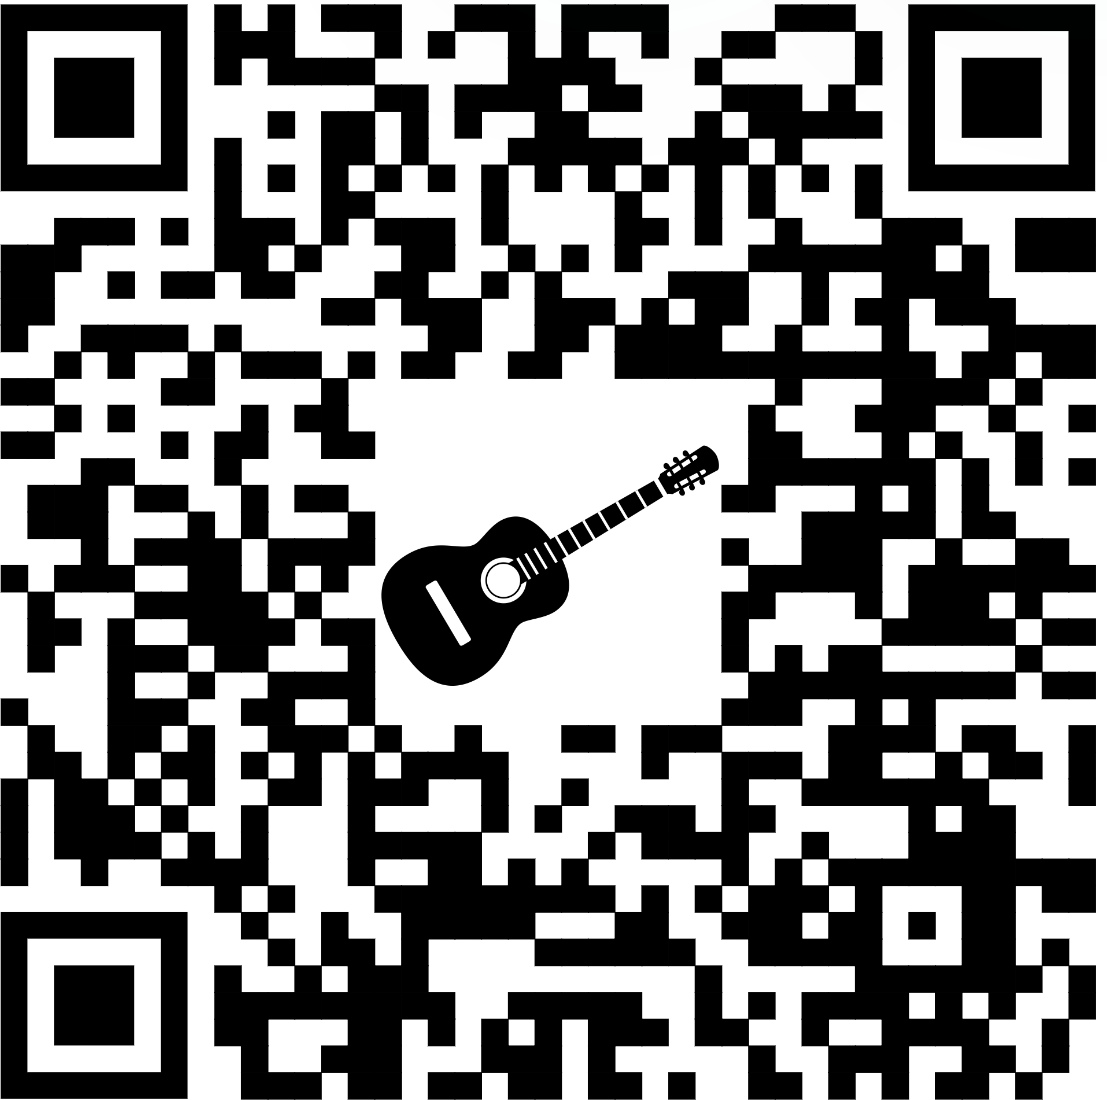
\includegraphics[width=0.3\textwidth]{imgs/qrPisnicky.png}
\end{center}
\end{document}

% \documentclass{article}

% \usepackage[T1]{fontenc}
% \usepackage[utf8]{inputenc}

% \usepackage{songs}

% \newindex{titleidx}{titleidx}
% \newauthorindex{authidx}{authidx}

% \begin{document}

% \showindex[2]{Índex de títols}{titleidx}
% \showindex[2]{Índex de d'autors}{authidx}

% \begin{songs}{titleidx,authidx}

% \beginsong{Mi alma glorifica al Señor, mi Dios}[by={Tradicional}]

% \begin{chorus}
% Mi \[E]alma glorifica al Señor, mi \[B7]Dios,
% \[C#m]gózase mi espíritu en mi Salva\[G#m]dor.
% \[A]El es mi ale\[B7]gría, \[E]es mi pleni\[C#m]tud,
% \[A6]El es todo \[B7]para \[E]mí.
% \end{chorus}

% \begin{verse}
% \[G#] Ha mi\[C#m]rado la ba\[G#]jeza de su es\[C#m]clava,
% muy di\[B7]chosa me dirán todos los \[E]pueblos
% porque en \[C#7]mí ha hecho grandes mara\[F#m]villas
% El que \[C#m]todo puede, \[G#]cuyo Nombre es \[C#m]Santo. \[B7]
% \end{verse}

% \endsong

% \end{songs}

% \end{document}